\documentclass{amsart}
%\usepackage[backend=bibtex8,style=numeric,giveninits=true]{biblatex}
%\addbibresource{formschub.bib}
\usepackage{algorithm}
\usepackage{algpseudocode}
\usepackage{hyperref}
\usepackage{fancyvrb}
\usepackage{amsmath}
\usepackage{amsfonts}
\usepackage{amsthm}
\usepackage{amssymb}
\usepackage{array}
\usepackage{cases}
\usepackage{caption}
\usepackage{xcolor}
\usepackage{tikz}
\usepackage{tikz-cd}
\usepackage{mathtools}
\usetikzlibrary{calc}
\usepackage{centernot}
\usepackage{mathtools}
\usepackage{graphicx}
\usepackage[margin=1in]{geometry}
\usepackage[makeroom]{cancel}
\usepackage{stmaryrd}
\usepackage{stackengine}
\usepackage{mathrsfs}

%\usepackage{unicode-math}
%\usepackage{nicematrix}

%\usepackage{witharrows}

\newtheorem{lemma}{Lemma}[subsection]
\newtheorem{corollary}[lemma]{Corollary}
\newtheorem{conjecture}[lemma]{Conjecture} 
\newtheorem{proposition}[lemma]{Proposition} 
\newtheorem{theorem}{Theorem}[section]
\newtheorem{observation}{Observation}[section]
\newtheorem{question}{Question}

%\newtheorem{conj}[thm]{Conjecture} 


%%% 
%%% The following gives definition type environments (which only differ
%%% from theorem type invironmants in the choices of fonts).  The
%%% numbering is still tied to the theorem counter.
%%% 

\theoremstyle{definition}
%\newtheorem{definition}{Definition}[section]
%\newtheorem{example}{Example}[section]
\newtheorem{definition}[lemma]{Definition}
\newtheorem{example}[lemma]{Example}
%\newtheorem{algorithm}{Algorithm}
\newtheorem*{note}{Note}

%%
%% Again more of these can be added by uncommenting and editing the
%% following. 
%%

%\newtheorem{note}[thm]{Note}


%%% 
%%% The following gives remark type environments (which only differ
%%% from theorem type invironmants in the choices of fonts).  The
%%% numbering is still tied to the theorem counter.
%%% 


\theoremstyle{remark}

\newtheorem*{remark}{Remark}


%%%
%%% The following, if uncommented, numbers equations within sections.
%%% 

%\numberwithin{equation}{section}
\numberwithin{equation}{subsection}


%%%
%%% The following show how to make definition (also called macros or
%%% abbreviations).  For example to use get a bold face R for use to
%%% name the real numbers the command is $\mathbf{R}.  To save typing we
%%% can abbreviate as

\newcommand{\R}{\mathbf{R}}  % The real numbers.

%%
%% The comment after the defintion is not required, but if you are
%% working with someone they will likely thank you for explaining your
%% definition.  
%%
%% Now add you own definitions:
%%

%%%
%%% Mathematical operators (things like sin and cos which are used as
%%% functions and have slightly different spacing when typeset than
%%% variables are defined as follows:
%%%

\DeclareMathOperator{\sch}{\mathfrak{S}}
\newcommand{\shup}{{\uparrow}}
\newcommand{\downvar}[1]{\stackrel{#1}{\searrow}}
\newcommand{\wof}[1]{w_{#1}}
\newcommand{\rcdd}{\mathfrak{F}}
\newcommand{\wtt}{\mathtt{wt}}
\newcommand{\tom}[1]{\xrightarrow{#1}}
\newcommand{\Tom}[1]{\xRightarrow{#1}}
\newcommand{\mot}[1]{\xleftarrow{#1}}
\newcommand{\cperm}[1]{\llbracket #1\rrbracket}
\newcommand{\cpcf}[5]{d^{#1,#2}_{#3}\left(#4\mid #5\right)}
% simplified product notation
\newcommand{\smpfu}{\mathsf{\Pi}}
\newcommand{\smpr}[3]{\ensuremath{}\smpfu\left( #1 \mid #2_{[#3]}\right)}
\newcommand{\smpre}[2]{\ensuremath{}\smpfu\left( #1 \mid #2\right)}
\newcommand{\rtt}{\mathtt{rt}}
\newcommand{\trm}{\mathtt{trim}}
\newcommand{\zeromap}{\mathcal{Z}}
\newcommand{\hr}{\mathtt{ht}}
%\newcommand{\shifthom}{\operatornamewithlimits{\raisebox{1ex}{$\stackrel{\blacktriangleright}{\mathbf{\_}}$}}\limits}

%\newcommand{\shifthom}{\operatornamewithlimits{\raisebox{1ex}{$\blacktriangleright$}}\limits}

\newcommand{\shifthom}{\operatornamewithlimits{\triangleright}\limits}


%\newcommand{\shiftvby}[1]{\ensuremath{\resizebox{\width}{\heightoff}{$\shifthom_{#1}$}}}

\newcommand{\shiftvby}[1]{\shifthom_{#1}}

\newcommand*\circled[1]{%
	\tikz[baseline=(char.base)]{
		\node[shape=circle,draw,inner sep=0.1pt] (char) {#1};
	}%
}
\newcommand\mycircled[1]{\makebox[0pt]{\circled{#1}}}
\newcommand{\tb}{\textbullet}
\newcommand{\xr}[1]{\ensuremath{{}\xrightarrow{[#1]}{}}}
\newcommand{\rd}[1]{\ensuremath{\mathcolor{red}{\mathbf{#1}}}}
\newcommand{\mc}[1]{\ensuremath{\mycircled{#1}}}
\newcommand{\desc}{\mathrm{Desc}}%
%\newcommand{\schv}[2]{\operatornamewithlimits{\sch_{\mathit{#2}}}\limits_{\negphantom{{}_{\mathit{#2}}}\negvphantom{{}_{\mathit{#2}}}#1}}

%\newcommand{\schv}[2]{\setstackgap{S}{0pt}\setstackgap{L}{0pt}\stackMath\stackunder{\sch_{#2}}{\negphantom{\scriptstyle{#2}}\!{\scriptscriptstyle{#1}}}}

\newcommand{\schv}[2]{\shiftvby{#1}\!\sch_{#2}}

%\newcommand{\shiftvby}[1]{\makebox[0pt]{$\triangleright$}#1}



%\newglossary[slg]{symbolslist}{syi}{syg}{List of symbols}
%\makeglossaries

%\begin{itemize}
%	\item Elements of $S_\infty$ $c{[}p,q{]}$, $d{[}p,q{]}$, $r{[}p,q{]}$, homomorphism $\sigma_p:S_\infty\to S_\infty$: Definition \ref{definition:specelem}	

%	\item  Relations between elements of $S\infty$ $\tom{k},\Tom{k}$: Definition \ref{definition:pierisymb}

%	\item Code, dual code, $\code(w)$, $\code^*(w)$, dominant permutations, the dominant approximation $\dom(v)$: Definition \ref{definition:codestuff}

%	\item Function/sets of permutations related to pulling out variables from Schubert polynomials $\varphi_{i,n}$, $\mathcal{D}_i(v)$, $Q_i(v',v)$: Definition \ref{definition:polysequence}

%	\item Flattening function $\phi_i:S_\infty\to S_\infty$, domination relation between permutations: Definition \ref{definition:domination}

%	\item Special polynomials $H_p(x;y)$, $E_p(x;y)$, $\smpr{x_1}{y}{p}$: Definition \ref{definition:hp}

%	\item Polynomial variable omission $x^{(i)}$, subscript substitution $y_A$, index shift function $\shiftvby{i}$: Definition \ref{definition:pv}
%\end{itemize}

\newcommand{\dsch}{\ensuremath{\Xi}}
\newcommand{\coma}{\mathcal{A}}
\newcommand{\dcoma}{\mathcal{D}}



%%
%% This is the end of the preamble.
%% 
\title{The Schubert Algebra and the ring of RC graphs}
\author{Matthew J. Samuel}

%\newcommand{\tomm}[2]{\xrightarrow{#1}_{#2}}
%\counterwithout{equation}{section}
%\setcounter{section}{-1}
\newcommand{\shuff}[2]{\mathcal{S}\mathcal{H}_{#1}^{#2}}
\newcommand{\dom}{\mathfrak{d}}
\newcommand{\ldom}{\dom^*}
\newcommand{\code}{\mathfrak{c}}
\newcommand{\ducode}{\overline{\mathfrak{c}}}

\newcommand{\maxd}{\mathfrak{m}}
\newcommand{\ddv}[1]{{{}_{{\scriptscriptstyle (#1)}}\partial}}
%\newglossary[slg]{symbolslist}{syi}{syg}{Symbolslist}
%\GlsXtrLoadResources
%[src={symbols},sort=use,type=main,
%	group=specelem]
%\glsaddstoragekey{group}{}{\grouplabel}
%\glsxtrsetgrouptitle{specelem}{}





%\newglossary[slg]{symbol}{sot}{stn}{Symbols}
%\makeglossaries

\begin{document}
	\maketitle
	
\section{Some preliminaries}
\subsection{Notation}
\begin{definition} \label{definition:polysequence}
		For a permutation $v'$ such that $v'\in S_{n}$, define
		$$\varphi_{i,n}(v')(j)=\begin{cases}
			v'(j)&\mbox{ if }j<i\\
			n+1&\mbox{ if }j=i\\
			v'(j-1)&\mbox{ if }i<j\leq n+1\\
			j&\mbox{ if }j>n+1
		\end{cases}$$
		Now fix $v\in S_n$ and $i\geq 1$ an integer, we define a relation $\downvar{i}$ by declaring that $v\downvar{i} v'$ if 
		$$v\Tom{i}\varphi_{i,n}(v')$$
		Equivalently, $v\downvar{i} v'$ if whenever $v\in S_n$ and $n$ is minimal, we have that $v$ satisfies the relation $\Tom{i}$ with respect to the permutation obtained from $v'$ by inserting $n+1$ at position $i$. We note that this concept was introduced by Bergeron and Sottile in \cite{bsskew}.
		
		If $v\downvar{i} v'$, we define a set of integers $Q_i(v',v)$ by
		$$Q_i(v',v)=\{v(j)\mid j>i\mbox{ and }v'(j-1)=v(j)\}$$
		Given the fact that any element of $S_\infty$ fixes all but finitely many positive integers, it follows that $Q_i(v',v)$ is a finite set.
		
		We then define $\mathcal{D}_i(v)$ to be all permutations $v'\in S_\infty$ such that $v\downvar{i} v'$. The permutations $\mathcal{D}_i(v)$ arise when pulling a variable out of a Schubert polynomial and expressing the coefficients of the powers of this variable as Schubert polynomials in the remaining variables, as is done in \cite{coprod}, from which this definition essentially comes.

		For a permutation $v\in S_\infty$, we define $\shup{v}$ to be the permutation defined by
		$$\shup{v}(i) = \begin{cases}
			v(i-1)+1&\mbox{ if }i>1\\
			1&\mbox{ if }i=1
		\end{cases}$$
		Recursively, we define $\shup^k(v)$ to be $\shup(\shup^{k-1}(v))$.

		For a permutation $w$, we define $\maxd(w)$ to be the maximum right descent of $w$. That is
		$$\maxd(w) = \max\{i\mid w(i)>w(i+1)\}$$

		Define
		$$\smpre{a}{B} = \prod_{b\in B}(a-b)$$
	\end{definition}

	\begin{proposition}[Special case of Pieri formula {\cite[Theorem~7.1]{samuelmolev}}] \label{proposition:pieri}
Suppose $k\geq 1$ and $u,w\in S_\infty$. If $u\not\tom{k} w$, then
$$\ddv{y}_u^w\smpr{x_1}{y}{k}=0$$
If $u\tom{k} w$, define
$$Q = \{u(i)\mid i\leq k\mbox{ and }u(i)=w(i)\}$$
then
$$\ddv{y}_u^w\smpr{x_1}{y}{k}=\smpre{x_1}{y_Q}$$
\end{proposition}
\begin{proof}
	This is simply a change of variables from the original theorem.
\end{proof}

The next proposition specializes, in the case of ordinary Schubert polynomial $\sch_v(x)$, to a formular that isolate a chosen index $i$: one can express $\sch_v(x)$ as a sum of terms of the form $x_i^p\sch_{v'}(x^{(i)})$, thereby effectively extracting the variable $x_i$ and leaving Schubert polynomials in the remaining variables \cite[Theorem~5.1]{bsskew}. Proposition \ref{proposition:pullindex} is the double Schubert polynomial version of this, which, as far as we know, is new.% A more general formula is possible for arbitrary splitting into disjoint sets of indices, similar to the formula in \cite{bsskew} and using the same method of proof as Proposition \ref{proposition:pullindex} coupled with the main result of \cite{samuelleibniz}, though we will not need this here.


\begin{proposition} \label{proposition:pullindex}
Let $v\in S_\infty$ and let $i>0$ be an integer. Then we have
$$\sch_v(x;y)=\sum_{v\downvar{i} v'}\smpre{x_i}{y_{Q_i(v',v)}}\sch_{v'}(x^{(i)};y)$$
\end{proposition}
\begin{proof}
Suppose $v\in S_n$. We have
$$\sch_v(x;y)=\ddv{y}^{vw_0(n)}(\sch_{w_0(n)}(x;y))$$
This is equal to
$$\ddv{y}^{vw_0(n)}(\sch_{s_{n+1-i}\cdots s_1w_0(n)}(x^{(i)};y)\smpr{x_i}{y}{n+1-i})$$
and, applying the Leibniz formula, is also equal to
$$\sum_{\substack{v'\in S_\infty\\\ell(v'w_0(n)s_1\cdots s_{n+1-i})=\ell(w_0(n)s_1\cdots s_{n+1-i})-\ell(v')}}\sch_{v'}(x^{(i)};y)\ddv{y}_{v'w_0(n)s_1\cdots s_{n+1-i}}^{vw_0(n)}\smpr{x_i}{y}{n+1-i}$$
By the restricted Pieri formula (Proposition \ref{proposition:pieri}), for this to be nonzero necessarily $v'w_0(n)s_1\cdots s_{n+1-i}\tom{n+1-i}vw_0(n)$. We note that $v'w_0(n)s_1\cdots s_{n+1-i}\tom{n+1-i}vw_0(n)$ if and only if 
$$v\Tom{i}v'w_0(n)s_1\cdots s_{n+1-i}w_0(n)=v's_ns_{n-1}\cdots s_i$$
We have that $v's_n\cdots s_i$ is exactly $\varphi_{i,n}(v')$ since $v'\in S_n$, so we require that
$$v\Tom{i}\varphi_{i,n}(v')$$
so the sum is over all $v'\in \mathcal{D}_i(v)$.

Applying Proposition \ref{proposition:pieri}, we obtain that the result is equal to
$$\sum_{v'\in \mathcal{D}_i(v)} \smpre{x_i}{y_{A(v',v)}}\sch_{v'}(x^{(i)};y)$$
where $A(v',v)$ is the set of all $vw_0(n)(j)$ such that $1\leq j\leq n+1-i$ and $v'w_0(n)s_1\cdots s_{n+1-i}(j)=vw_0(n)(j)$. These values are the same as at the indices that comprise the set of all $1\leq j\leq n+1-i$ such that
$$v'(n+2-s_1\cdots s_{n+1-i}(j))=v(n+2-j)$$
Applying the $s_1\cdots s_{n+1-i}$ to $j$, since $1\leq j\leq n+1-i$ we have that 
$$s_1\cdots s_{n+1-i}(j)=j+1$$
Hence we need
$$v'(n+2-(j+1))=v'(n+1-j)=v(n+2-j)$$
Replacing $j$ with $n+2-p$, the indices are the set of all $p$ such that $i<p\leq n+1$ and
$$v'(p-1)=v(p)$$
Thus $A(v',v)$ is the set of all $v(p)$ such that $p>i$ and $v'(p-1)=v(p)$, which is exactly $Q_i(v',v)$, and we are done.
\end{proof}


\section{The Schubert Algebra and its dual}

\subsection{Definition}


We define a commutative algebra $\coma$ over the integers as follows. For each $n$, define $\coma_n$ to be the polynomial ring over $\mathbb{Z}$ in the variables $x_1,\ldots,x_n$. Then define
$$\coma =\bigoplus_{n=0}^\infty \coma_n$$
The multiplication within $\coma_n$ is as usually defined for the polynomial ring. However, if $a\in \coma_m$ and $b\in \coma_n$ with $m\neq n$ and $m,n>0$,  then
$$ab = 0$$
Otherwise, the component for $n=0$ is identified with the coefficient ring. Note that the ``identity element'' for positive $n$ is not an identity element of $\coma$ (we may sometimes refer to it as a ``fat identity'').

Each $\coma_n$ has a basis consisting of elements $x_a^{(n)}$, where $a$ is a sequence of $n$ nonnegative integers, and the notation indicates that
$$x_a = x_1^{a_1}\cdots x_n^{a_n}$$
The direct sum therefore has a basis that can canonically be identified with union of these.

We define a coproduct $\Delta:\coma\to\coma\otimes\coma$ on the basis $x_c^{(n)}$ by
$$\Delta(x_c^{(n)}) = \sum_{\substack{p+q=n\\ab=c}} x_a^{(p)}\otimes x_b^{(q)}$$
where the equation $ab=c$ indicates that $a$ concatenated with $b$ is equal to $c$. We also define a counit $\varepsilon:\coma\to \mathbb{Z}$ by $\varepsilon(x_a^{(n)})=0$ unless $n=0$.

\begin{lemma}
	With $\Delta$ and $\varepsilon$, $\coma$ is a coassociative, counital coalegebra.
\end{lemma}
\begin{proof}
	We have 
	$$\Delta(x_d^{(n)})=\sum x_a^{(p)}\otimes x_c^{(q)}$$
	Applying $\Delta$ to either tensor factor results in
	$$\sum x_a^{(p)}\otimes x_b^{(q)}\otimes x_c^{(r)}$$
	The symmetry of this is exactly the coassociativity condition. Seeing that we may choose $p=n$ or $q=n$, the definition of the counit gives us the result that $\coma$ is counital as well under $\Delta$ and $\varepsilon$.
\end{proof}

\begin{lemma}
	$\Delta:\coma\to\coma\otimes\coma$ is a homomorphism of rings.
\end{lemma}
\begin{proof}
	This is where the condition that $x_a^{(p)}x_b^{(q)}=0$ unless $p=q$ when both $p,q>0$ comes in. It ensures that only monomials of the same length have nonzero products and preserves the structure of the coproduct as a homomorphism of rings.
\end{proof}

\begin{lemma}
	$\nabla:\coma\otimes \coma\to \coma$ is a homomorphism of coalgebras.
\end{lemma}
\begin{proof}
	
\end{proof}

\begin{corollary}
	$\coma$ is a bialgebra over $\mathbb{Z}$.
\end{corollary}

$\coma$ is afforded a grading into finite dimensional components by observing that each $\coma_n$ itself is a graded ring with each homogeneous component being a finitely generated free module. Considering the pair $(n, d)$, where $n$ is the number of variables and $d$ is the degree, as a $\mathbb{Z}^2$ grading, we may take the graded dual module $\dcoma$, which, by virtue of the grading, is isomorphic as a free module to $\coma$. We identify the dual basis element $x_a^*$ with the sequence of nonnegative integers $a$. That is to say,
$$\langle a, x_b\rangle = \delta_{ab}$$
Inspection of the coproduct reveals that the product of $a$ and $b$ in $\dcoma$ is simply the concatenation $ab$. Hence $\dcoma$ is isomorphic to the free associative algebra on a countable set indexed by nonnegative integers.

$\dcoma$ also has a coproduct compatible with its product, namely
$$c\mapsto \sum_{a+b=c} a\otimes b$$
Thus $\coma$ and $\dcoma$ are dual bialgebras.

Calling $\coma$ the ``Schubert algebra'' may seem unnecessarily grandiose, however the reason will become clear below.

\subsection{The Schubert basis}

In $\coma$, each $\coma_n$ has a basis of Schubert polynomials $\sch_u^{(n)}$, where the largest right descent of $u$ is at most $n$, ensuring that $\sch_u(x)$ has at most $n$ variables. Schubert polynomials limited to a specific number of variables have well-defined structure constants $c_{u,v}^w$, independent of $n$, given by
$$\sch_u^{(n)}\sch_v^{(n)} = \sum_{w}c_{u,v}^w\sch_w^{(n)}$$
These are known to be nonnegative integers, however except in special cases no positive combinatorial formula is known.

Schubert polynomials have nonnegative coefficients in terms of the $x_a^{(n)}$ basis, for which many formulas are known. There is also a less well-understood unique expansion of the Schubert polynomials into sums of products of elementary symmetric polynomials with at most $n$ variables. 

\newcommand{\sdom}{\widetilde{\mu}}


\subsection{The elementary basis}

for all $i>n$, satisfying the additional restriction that $\alpha_i\geq \alpha_{i+1}$ if $i\geq n$.

An $n$-elementary monomial is a an element of the polynomial ring of the following form: 
$$e_{\alpha_1}^{1}\cdots e_{\alpha_n}^ne_{\alpha_{n+1}}^n\cdots e_{\alpha_m}^n$$
where $\alpha$ is an $n$-elementary weak composition. Define $\mathcal{E}_n$ to be the set of $n$-elementary monomials.

\begin{theorem}
	$\mathcal{E}_n$ forms a $\mathbb{Z}$-basis for $\coma_n$, and $\bigcup_{n}\mathcal{E}_n$ forms a basis for $\coma$.
\end{theorem}
\begin{proof}
	It is a theorem of Macdonald that the polynomial ring $\mathbb{Z}[x_1,\ldots,x_n]$ is a free module over $\Lambda_n$ with basis the Schubert polynomials $\sch_u(x)$ such that $u\in S_n$. These Schubert polynomials are uniquely expressed in terms of strict elementary symmetric monomials with fewer than $n$ variables. Since $\Lambda_n$ is a polynomial ring in the $e_{i,n}$ by the fundamental theorem of elementary symmetric polynomials, $\Lambda_n$ has a basis of monomials $e_{\lambda,n}$ as $\lambda$ ranges over all partitions with parts bounded by $n$. The multiplicative combination of these two bases is therefore a $\mathbb{Z}$-basis of $\coma_n$. This is exactly the description of the monomials $e_{\alpha}^n$ for $\alpha$ an $n$-elementary weak composition.
\end{proof}

We can ask for transition formulas between the Schubert and the elementary basis. From elementary to Schubert, we may use Sottile's Pieri formula. That is,

$$e_{\alpha}^n = \sum_{1\xrightarrow{1,2,\ldots,n}_{\alpha} u}\sch_u^n$$

For the reverse transition, suppose we want to express $\sch_w^n$ in the elementary basis. Let $\lambda = \mu^*_n(w)$ and consider the double Schubert polynomial
$$\sch_{\lambda}(x;y)=\prod_i E_{\lambda_i}(x;y_i)$$
We have that
$$\sch_w(x;y) = \partial_y^{w\lambda^{-1}}\sch_\lambda(x;y)$$
Applying the Leibniz formula, this is
$$\sum_{u_0\xrightarrow{1} u_1\cdots}\prod_i \partial^{u_i/u_{i-1}}_yE_{\lambda_i}(x;y_i)$$
It is possible to find a combinatorial formula for each factor in the product, keeping the $y$ variables, but we only need the sign. We define $\sigma_i(u_{i-1},u_i)$ to be the number of indexes $j<i$ such that $u_{i-1}(j)\neq u_i(j)$. Then we define
$$\sigma(P)=\sum_i \sigma_i(u_{i-1},u_i)$$
%$$\sch_w^n = \sum_{P:1\xrightarrow{\lambda} w\lambda^{-1}} (-1)^{|\lambda| - \ell(w) + \sigma(P)}e_{\alpha(P,\lambda),\lambda}^n$$
Then we define
$$E^{\alpha;n}_w = \sum_{\substack{P:1\xrightarrow{\lambda} w\lambda^{-1}\\\alpha(P)=\alpha}}(-1)^{|\lambda|-\ell(w)+\sigma(P)}$$

\begin{theorem}
	For each $w$, we have
	$$\sch_w^n = \sum_{\alpha}E_w^{\alpha;n}e_{\alpha}^n$$
\end{theorem}
These numbers are stable for fixed $w$ as soon as the number of variables is at least as large as the value of $n$ such that $w\in S_n$, and are well-studied but poorly understood.

\begin{example}
	Let $n=5$ and let $w$ be the permutation such that $\code(w)=(0,2,0,2,3)$. Let $\lambda = (5,5,5,4,3,2,1)$. Then
	\begin{align*}
		\sch_w^n &= e_{(0,0,0,0,5,1,1)} - e_{(0,0,0,0,4,2,1)} + e_{(0,0,0,0,4,3)}- e_{(0,1,0,0,4,1,1)} +e_{(0,0,1,0,3,2,1)}\\
		&+e_{(0,1,0,0,5,1)} + e_{(0,1,0,0,3,3)}
	\end{align*}
\end{example}
%\section{The Schur-elementary basis}

%$\Sigma_n$
%$$c_{u,\lambda^{\perp,m}}^{w\mu_{n,m}w_0(n-1)}E_{u,a}^ns_{\lambda}(x_1,\ldots,x_n)e_{a}$$

%Express $w_0(n,m)$ as $\sch_{w_(n-1)}(x)E_n(x)^m$.

% e_3e_3e_2e_1
Suppose $\alpha$ and $\beta$ are weak compositions. We define $\alpha\|_p \beta$ to be the weak composition defined by
$$\gamma_i = \begin{cases}
	\alpha_i&\mbox{ if }i\leq p\\
	\alpha_i + \beta_{i-p}&\mbox{ if }i> p
\end{cases}$$

\begin{theorem}
	$$\Delta(e_\gamma^n) = \sum_{\substack{\alpha \|_p \beta=\gamma\\p+q=n}} e_{\alpha^{\overline{p}}}^p\otimes e_\beta^q$$
	where $\alpha$ ranges over all weak compositions such that $\alpha^{\overline{p}}$ is $p$-elementary and $\beta$ ranges over all $q$-elementary weak compositions.
\end{theorem}

\subsection{The Schubert-Schur and separated descents basis}

%Schur-Schubert structure constants are positive, and the Schubert basis is positive in the Schur-Schubert basis.

$\coma_n$ has a basis of the form $S_{\lambda,u}^n=s_\lambda(x_1,\ldots,x_n)\sch_u(x)$, where $u\in S_n$ and $s_\lambda$ is the Schur polynomial corresponding to $\lambda$ in $\Lambda_n$. This is called the \emph{Schubert-Schur} basis. There is a generalization that this is an easy special case of that can be described as follows.
%$$S_{\lambda,u}^n = \sum c_{v_{\lambda;n},u}^{w}\sch_w^n$$

%Thus

%$$\dsch_w^n = c_{v_{\lambda;n},u}^w\Omega_{\lambda,u}^n$$

%\section{The separated descents basis}

Let $K_{u,v;k}^n = \sch_u(x_1,\ldots,x_n)\sch_v(x_1,\ldots,x_{k-1})$, where $v\in S_k$ and $u$ is a permutation such that $\ell(us_i)>\ell(u)$ for all $i<k$. We will call this the \emph{separated descents basis} for the descent $k$.

\begin{theorem}
	For fixed $k$, $K_{u,v;k}^n$ form a basis of $\coma_n$ for all $n\geq k$.
\end{theorem}
\begin{proof}
	First we show that these elements additively generate the subring. Note first that $\mathcal{E}_n$ is a basis. Let $e_{\alpha_1}^{\lambda_1}\cdots e_{\alpha_m}^{\lambda_m}\in \mathcal{E}_n$. Let $j$ be the index such that $\lambda_j=k$. Let
	$$P=\prod_{i=1}^j e_{\alpha_i}^{\lambda_i}$$
	and let
	$$Q=\prod_{i=j+1}^{m} e_{\alpha_i}^{\lambda_i}$$
	By the fact that $\lambda_{i-1} = \lambda_i +1$ for all $i>j$, it follows that
	$$Q=\sum c_v\sch_{v}(x)$$
	for integers $c_v$ with $v\in S_k$. Given the fact that $P$ is symmetric in $x_1,\ldots,x_k$, it can be shown that
	$$P=\sum d_u\sch_u(x)$$
	for integers $d_u$ and permutations $u\in S_\infty$ with $\ell(us_i)>\ell(u)$ for all $i<k$. Thus the $n$-elementary monomial can be expressed as
	$$PQ=\sum c_ud_v\sch_u(x_1,\ldots,x_n)\sch_v(x_1,\ldots,x_{k-1})$$
	Since the $n$-elementary monomials form a basis, this proves that $K_{u,v;k}^n$ spans $\coma_n$.
	
	To prove independence, first note that if 
	$$\sum_{u} c_{u}K_{u,1;k}^n = \sum_u c_u\sch_u(x)= 0$$
	then $c_u=0$ for all $u$ by independence of Schubert polynomials. Assume the inductive hypothesis that for some $m>0$ we have that if 
	$$\sum_u c_{uv}K_{u,v;k}^n=0$$ 
	and for all $v$ in the sum with $\ell(v)\geq m$ we have $c_{uv}=0$, then $c_{uv}=0$ for all $u$ and $v$. For a sum with possibly nonzero terms such that $\ell(v)=m$ at most, suppose
	$$\sum_{u,v} c_{u,v}K_{u,v;k}^n = 0$$
	Let $i$ be a positive integer. Then by applying the divided difference $\partial^{s_i}$ we see that
	$$\sum_{u,v} c_{u,v}K_{u,vs_i;k}^n = 0$$
	for all $v$ with $\ell(vs_i)<\ell(v)$. In particular, the maximum length with a possibly nonzero coefficient has decreased by at least $1$. By the inductive hypothesis, all terms in this sum are $0$, hence $c_{uv}=0$ for all $u$ and $v$ with $\ell(vs_i) < \ell(v)$. Iterating over all $i$, we have the result.
\end{proof}

For transition coefficients, expressing $K_{u,v;k}^n$ in terms of Schubert polynomials is ``easy'' and combinatorially known to have nonnegative coefficients. While positive formulas are known, their discovery is quite recent.

Expressing the Schubert basis in terms of $K_{u,v;k}^n$ can be done as follows.

Recall we can express $\sch_w^n$ as
$$\sch_w^n = \sum_{\alpha} E_w^{\alpha;n}e_{\alpha}^n$$
To transition to the basis $K_{u,v;k}^n$, let $a$ be the index such that $\lambda_a = k$. Then
$$\sch_w^n = \sum_{\alpha} E_w^{\alpha;n}\left(\prod_{i=1}^a e_{\alpha_i,\lambda_i}\right)\left(\prod_{j=a+1}^{\ell(\lambda)} e_{\alpha_j,\lambda_j}\right)$$
These products can be expanded with the Pieri formula as
$$\sch_w^n = \sum_{\alpha}E_w^{\alpha;n}c_{\alpha',\lambda'}^uc_{\alpha'',\lambda''}^vK_{u,v;k}^n$$

\begin{example}
	Let $n=5$, let $k=3$, and let $w$ be the permutation such that $\code(w)=(0,2,0,2,3)$. Then
	$$\sch_w^n =K_{12468357, 132;3}^5 - K_{13468257, 1; 3}^5$$
	If instead we let $k=4$, we obtain
	$$\sch_w^n =-K_{124563, 132;4}^5+ K_{1246735, 132;4}^5+ K_{134562, 1;4}^5- K_{1346725, 1;4}^5+ K_{234561, 132;4}^5$$
\end{example}


\subsection{The dual algebra}

We examine the graded dual algebra $\dcoma$ more closely now. This is a graded ring generated by countably many elements that we denote by $[i]$, where $i$ is a nonnegative integer. The product, as mentioned previously, is concatenation of sequences. Thus
$$[a_1\cdots a_p][b_1\cdots b_q]=[a_1\cdots a_pb_1\cdots b_q]$$
It is not hard to see that $\dcoma$ is a free algebra on these generators. Thus the set of sequences $[a_1\cdots a_n]$ forms a $\mathbb{Z}$-basis for $\dcoma$. We may realize this as the dual of $\coma$ by declaring that
$$\langle [a_1\cdots a_n],x_1^{b_1}\cdots x_n^{b_n}\rangle = \prod_i\delta_{a_i,b_i}$$

We have a $\mathbb{Z}\times \mathbb{Z}$ grading such that
$$\deg([a_1\cdots a_n])=(n,-a_1-a_2\cdots-a_n)$$
The set of elements such that $\deg(a) = (n,-)$ is $\dcoma_n$, dual as a graded module to $\coma_n$.

\subsection{The dual Schubert basis}
       
There is a basis $\dsch_u^{n}$ dual to the Schubert basis for $\dcoma_n$. Specifically, with the unique pairing $\langle -,-\rangle:\dcoma\times \coma\to\mathbb{Z}$ such that
$$\langle \alpha,x_\beta\rangle = \delta_{\alpha\beta}$$
we define $\dsch_u^n$ to be the unique basis of $\dcoma_n$ such that
$$\langle \dsch_u^n,\sch_v^n\rangle = \delta_{uv}$$
We characterize it with an explicit formula.

\begin{theorem}
	For each permutation $u$ and integer $n$ with $\ell(us_i)>\ell(u)$ for all $i>n$ we have the equation
	$$\dsch_u^{n} = \sum_{\ell(\alpha)=n} E^{\code(\mu)-\alpha,\code(\mu)}_{u\mu^{-1}}\alpha$$
	where $\mu$ is any strict dominant permutation such that $0\neq \code_n(\mu) \geq \ell(u)$ and $\code_{n+1}(\mu)=0$.
\end{theorem}
\begin{proof}
	By definition, the coefficient of $\alpha$ in $\dsch_u^n$ is the coefficient of $\sch_u^n$ in $x_\alpha$. This can be derived from the Cauchy formula for double Schubert polynomials. Note that for any permutation $\mu$ as laid out in the statement of the theorem, $\ell(u\mu^{-1})=\ell(\mu)-\ell(u)$. Thus,
	$$\partial_y^{u\mu^{-1}}\sch_\mu(x;-y) = \sch_u(x;-y)$$
	We have that
	$$\sch_\mu(x;-y)=\sum_u \sch_u(x)\sch_{u\mu^{-1}}(y)$$
	Expressing the second factor in the $e_{\alpha,\lambda}(y)$ basis, we have
	$$\sch_\mu(x;-y)=\sum_{u,\alpha} \sch_u(x)E_{u\mu^{-1}}^{\code(\mu)-\alpha,\code(\mu)}e_{\code(\mu)-\alpha,\code(\mu)}(y)$$
	An alternative expression for $\sch_\mu(x;-y)$ is
	$$\sch_\mu(x;-y)=\sum_{\alpha} x_\alpha e_{\code(\mu)-\alpha,\code(\mu)}(y)$$
	from which we see that the coefficient is correct.
\end{proof}

% By definition, the coefficient of $\alpha$ in $\dsch_u^n(y)$ is the coefficient of $\sch_u^n(x;y)$ in $x_\alpha(y)$. This can be derived from the Cauchy formula for double Schubert polynomials. Note that for any permutation $\mu$ as laid out in the statement of the theorem, $\ell(u\mu^{-1})=\ell(\mu)-\ell(u)$. Thus,
% 	$$\partial_y^{u\mu^{-1}}\sch_\mu(x;y) = \sch_u(x;y)$$
% 	We have that
% 	$$\sch_\mu(x;y)=\sum_u \sch_u(x;z)\sch_{\mu u^{-1}}(z;y)$$
% 	Expressing the second factor in the $e_{\alpha,\lambda}(y)$ basis, we have
% 	$$\sch_\mu(x;-y)=\sum_{u,\alpha} \sch_u(x)E_{u\mu^{-1}}^{\code(\mu)-\alpha,\code(\mu)}e_{\code(\mu)-\alpha,\code(\mu)}(y)$$
% 	An alternative expression for $\sch_\mu(x;-y)$ is
% 	$$\sch_\mu(x;-y)=\sum_{\alpha} x_\alpha(z) e_{\code(\mu)-\alpha,\code(\mu)}(z;y)$$
% 	from which we see that the coefficient is correct.

This is not stable for fixed $u$ as $n$ increases, and this is expected.


\begin{example}
Suppose $w = [1,4,5,2,3]$. Then
$$\dsch_w^3 = [022] - [013]$$
If we chose $[1,3,5,7,2,4,6]$ instead, we have
$$\dsch_{1357246} = [0015] - [0033] - [0114] + [0123]$$
For $w=[4,2,7,1,3,5,6]$,
$$\dsch_{4271356}^3 = -[026] + [035] + [125] - [134] + [206] - [215] - [305] + [314]$$
\end{example}

\begin{lemma} \label{lemma:lexperm}
Let $w\in S_\infty$ and let $n\geq \maxd(w)$. Then
$$\dsch_w^n = [\code_1(w),\ldots,\code_n(w)] + \sum_{a <_{lex} \code(w)} c_a [a]$$
where the sum is over sequences of nonnegative integers $a$ of length $n$ that are lexicographically less than $\code(w)$.
\end{lemma}
\begin{proof}
Write
$$\alpha = \sum c_{\alpha, w}\dsch_w^n$$
Then for each $w$ we have that $\alpha\geq \code(w)$ in lexicographical order, due to the fact that $x^{\code(w)}$ is the lexicographically minimal monomial in $\sch_w(x)$, with a coefficient of exactly $1$. We thus have that the word basis is lower triangular in the Schubert basis, and vice versa. Since the coefficient of $x^{\code(w)}$ in $\sch_w(x)$ is $1$, the result follows.
\end{proof}

\begin{lemma}
	Let $u,v\in S_\infty$ and $p,q>0$ be integers. Write
	$$\dsch_u^p\dsch_v^q = \sum_w d_{u,v}^w(p,q)\dsch_w^{p+q}$$
	Then for each $u,v,w$ the coefficient $d_{u,v}^w(p,q)$ is the coefficient of $\sch_u(x_1,\ldots,x_p)\sch_v(x_{p+1},\ldots,x_{p+q})$ in the expansion of $\sch_w(x_1,\ldots,x_{p+q})$ in terms of the basis of products of Schubert polynomials in $x_1,\ldots,x_p$ and Schubert polynomials in $x_{p+1}$ onward.
\end{lemma}
\begin{proof}
	This is true by examination of the definition of the coproduct of $\coma$, since this is the coefficient of $\sch_u^p\otimes \sch_v^q$ in the coproduct of $\sch_w^{p+q}$.
\end{proof}

Thus the product structure of $\dcoma$ encodes splitting of the Schubert polynomial into two sets of variables. In particular,
\begin{lemma} \label{lemma:dpieri}
Let $a\geq 0$ be an integer and $w\in S_\infty$. Then we have
$$[a]\cdot \dsch_{w}^{n} = \sum_{\substack{w\in\mathcal{D}_1(w')\\\ell(w,w')=a}} \dsch_{w'}^{n+1}$$
\end{lemma}

We also have
\begin{lemma} \label{lemma:dpieriend}
Let $a\geq 0$ be an integer and $w\in S_\infty$. Then we have
$$\dsch_{w}^{n}\cdot [a] = \sum_{\substack{w\in\mathcal{D}_{n+1}(w')\\\ell(w,w')=a}} \dsch_{w'}^{n+1}$$
\end{lemma}


This is actually sufficient to get a full LR rule.

\begin{lemma}
Suppose
$$\dsch_u^p\dsch_v^q=\sum_{w}d_{u,v}^w(p,q)\dsch_w^{p+q}$$
Then
$$\dsch_u^p[0]^q=\sum_{\ell(w(\shup^{p}v)^{-1})=\ell(w)-\ell(v)}d_{u,v}^w(p,q)\dsch_{w(\shup^{p}v)^{-1}}^{p+q}$$
\end{lemma}

\begin{theorem} \label{theorem:LRdual}
Let $u,v\in S_\infty$ and $p,q>0$ be integers. Write
$$\dsch_u^p\dsch_v^q = \sum_w d_{u,v}^w(p,q)\dsch_w^{p+q}$$
Then $d_{u,v}^w(p,q)=0$ unless $\ell(w(\shup^{p}v)^{-1}) = \ell(w)-\ell(v)$ and $\ell(u)+\ell(v)=\ell(w)$. If these conditions are satisfied, then $d_{u,v}^w(p,q)$ is the number of sequences of permutations $(\sigma_0,\ldots,\sigma_q)$ such that $\sigma_0 = w(\shup^{p}v)^{-1}$, $\sigma_q = u$, and
$$\sigma_0\downvar{p+q}\sigma_2\downvar{p+q-1}\cdots \downvar{p+1}\sigma_{q}$$
\end{theorem}

\begin{example} \label{example:coproduct}
What is most interesting in this construction is the coproduct. Consider our example $w=[4,2,7,1,3,5,6]$. Using the word basis, it is a triviality to compute the coproduct $\Delta(\dsch_w^3)$:
\begin{align*}
&= - [000] \otimes [026] + [000] \otimes [035] + [000] \otimes [125] - [000] \otimes [134] + [000] \otimes [206] - [000] \otimes [215] \\
&\quad - [000] \otimes [305] + [000] \otimes [314] - [001] \otimes [025] + [001] \otimes [034] + [001] \otimes [124] - [001] \otimes [133] \\
&\quad + [001] \otimes [205] - [001] \otimes [214] - [001] \otimes [304] + [001] \otimes [313] - [002] \otimes [024] + [002] \otimes [033] \\
&\quad + [002] \otimes [123] - [002] \otimes [132] + [002] \otimes [204] - [002] \otimes [213] - [002] \otimes [303] + [002] \otimes [312] \\
&\quad - [003] \otimes [023] + [003] \otimes [032] + [003] \otimes [122] - [003] \otimes [131] + [003] \otimes [203] - [003] \otimes [212] \\
&\quad - [003] \otimes [302] + [003] \otimes [311] - [004] \otimes [022] + [004] \otimes [031] + [004] \otimes [121] - [004] \otimes [130] \\
&\quad + [004] \otimes [202] - [004] \otimes [211] - [004] \otimes [301] + [004] \otimes [310] - [005] \otimes [021] + [005] \otimes [030] \\
&\quad + [005] \otimes [120] + [005] \otimes [201] - [005] \otimes [210] - [005] \otimes [300] - [006] \otimes [020] + [006] \otimes [200] \\
&\quad - [010] \otimes [016] + [010] \otimes [025] + [010] \otimes [115] - [010] \otimes [124] - [010] \otimes [205] + [010] \otimes [304] \\
&\quad - [011] \otimes [015] + [011] \otimes [024] + [011] \otimes [114] - [011] \otimes [123] - [011] \otimes [204] + [011] \otimes [303] \\
&\quad - [012] \otimes [014] + [012] \otimes [023] + [012] \otimes [113] - [012] \otimes [122] - [012] \otimes [203] + [012] \otimes [302] \\
&\quad - [013] \otimes [013] + [013] \otimes [022] + [013] \otimes [112] - [013] \otimes [121] - [013] \otimes [202] + [013] \otimes [301] \\
&\quad - [014] \otimes [012] + [014] \otimes [021] + [014] \otimes [111] - [014] \otimes [120] - [014] \otimes [201] + [014] \otimes [300] \\
&\quad - [015] \otimes [011] + [015] \otimes [020] + [015] \otimes [110] - [015] \otimes [200] - [016] \otimes [010] - [020] \otimes [006] \\
&\quad + [020] \otimes [015] + [020] \otimes [105] - [020] \otimes [114] - [021] \otimes [005] + [021] \otimes [014] + [021] \otimes [104] \\
&\quad - [021] \otimes [113] - [022] \otimes [004] + [022] \otimes [013] + [022] \otimes [103] - [022] \otimes [112] - [023] \otimes [003] \\
&\quad + [023] \otimes [012] + [023] \otimes [102] - [023] \otimes [111] - [024] \otimes [002] + [024] \otimes [011] + [024] \otimes [101] \\
&\quad - [024] \otimes [110] - [025] \otimes [001] + [025] \otimes [010] + [025] \otimes [100] - [026] \otimes [000] + [030] \otimes [005] \\
&\quad - [030] \otimes [104] + [031] \otimes [004] - [031] \otimes [103] + [032] \otimes [003] - [032] \otimes [102] + [033] \otimes [002] \\
&\quad - [033] \otimes [101] + [034] \otimes [001] - [034] \otimes [100] + [035] \otimes [000] + [100] \otimes [025] - [100] \otimes [034] \\
&\quad + [100] \otimes [106] - [100] \otimes [115] - [100] \otimes [205] + [100] \otimes [214] + [101] \otimes [024] - [101] \otimes [033] \\
&\quad + [101] \otimes [105] - [101] \otimes [114] - [101] \otimes [204] + [101] \otimes [213] + [102] \otimes [023] - [102] \otimes [032] \\
&\quad + [102] \otimes [104] - [102] \otimes [113] - [102] \otimes [203] + [102] \otimes [212] + [103] \otimes [022] - [103] \otimes [031] \\
&\quad + [103] \otimes [103] - [103] \otimes [112] - [103] \otimes [202] + [103] \otimes [211] + [104] \otimes [021] - [104] \otimes [030] \\
&\quad + [104] \otimes [102] - [104] \otimes [111] - [104] \otimes [201] + [104] \otimes [210] + [105] \otimes [020] + [105] \otimes [101] \\
&\quad - [105] \otimes [110] - [105] \otimes [200] + [106] \otimes [100] + [110] \otimes [015] - [110] \otimes [024] - [110] \otimes [105] \\
&\quad + [110] \otimes [204] + [111] \otimes [014] - [111] \otimes [023] - [111] \otimes [104] + [111] \otimes [203] + [112] \otimes [013] \\
&\quad - [112] \otimes [022] - [112] \otimes [103] + [112] \otimes [202] + [113] \otimes [012] - [113] \otimes [021] - [113] \otimes [102] \\
&\quad + [113] \otimes [201] + [114] \otimes [011] - [114] \otimes [020] - [114] \otimes [101] + [114] \otimes [200] + [115] \otimes [010] \\
&\quad - [115] \otimes [100] + [120] \otimes [005] - [120] \otimes [014] + [121] \otimes [004] - [121] \otimes [013] + [122] \otimes [003] \\
&\quad - [122] \otimes [012] + [123] \otimes [002] - [123] \otimes [011] + [124] \otimes [001] - [124] \otimes [010] + [125] \otimes [000] \\
&\quad - [130] \otimes [004] - [131] \otimes [003] - [132] \otimes [002] - [133] \otimes [001] - [134] \otimes [000] + [200] \otimes [006] \\
&\quad - [200] \otimes [015] - [200] \otimes [105] + [200] \otimes [114] + [201] \otimes [005] - [201] \otimes [014] - [201] \otimes [104] \\
&\quad + [201] \otimes [113] + [202] \otimes [004] - [202] \otimes [013] - [202] \otimes [103] + [202] \otimes [112] + [203] \otimes [003] \\
&\quad - [203] \otimes [012] - [203] \otimes [102] + [203] \otimes [111] + [204] \otimes [002] - [204] \otimes [011] - [204] \otimes [101] \\
&\quad + [204] \otimes [110] + [205] \otimes [001] - [205] \otimes [010] - [205] \otimes [100] + [206] \otimes [000] - [210] \otimes [005] \\
&\quad + [210] \otimes [104] - [211] \otimes [004] + [211] \otimes [103] - [212] \otimes [003] + [212] \otimes [102] - [213] \otimes [002] \\
&\quad + [213] \otimes [101] - [214] \otimes [001] + [214] \otimes [100] - [215] \otimes [000] - [300] \otimes [005] + [300] \otimes [014] \\
&\quad - [301] \otimes [004] + [301] \otimes [013] - [302] \otimes [003] + [302] \otimes [012] - [303] \otimes [002] + [303] \otimes [011] \\
&\quad - [304] \otimes [001] + [304] \otimes [010] - [305] \otimes [000] + [310] \otimes [004] + [311] \otimes [003] + [312] \otimes [002] \\
&\quad + [313] \otimes [001] + [314] \otimes [000]
\end{align*}
Reexpressing this in the dual Schubert basis, e.g. with Lemma \ref{lemma:dpieri}, we have 
\begin{align*}
&= 1 \otimes \Xi_{4271356}^{3} + \Xi_{1243}^{3} \otimes \Xi_{3271456}^{3} + \Xi_{1243}^{3} \otimes \Xi_{4172356}^{3} + \Xi_{1243}^{3} \otimes \Xi_{426135}^{3} \\
&\quad + \Xi_{12534}^{3} \otimes \Xi_{3172456}^{3} + \Xi_{12534}^{3} \otimes \Xi_{326145}^{3} + \Xi_{12534}^{3} \otimes \Xi_{416235}^{3} + \Xi_{12534}^{3} \otimes \Xi_{42513}^{3} \\
&\quad + \Xi_{126345}^{3} \otimes \Xi_{316245}^{3} + \Xi_{126345}^{3} \otimes \Xi_{32514}^{3} + \Xi_{126345}^{3} \otimes \Xi_{41523}^{3} + \Xi_{126345}^{3} \otimes \Xi_{4231}^{3} \\
&\quad + \Xi_{1273456}^{3} \otimes \Xi_{31524}^{3} + \Xi_{1273456}^{3} \otimes \Xi_{4132}^{3} + \Xi_{1273456}^{3} \otimes \Xi_{4213}^{3} + \Xi_{132}^{3} \otimes \Xi_{3271456}^{3} \\
&\quad + \Xi_{132}^{3} \otimes \Xi_{4172356}^{3} + \Xi_{1342}^{3} \otimes \Xi_{3172456}^{3} + \Xi_{1342}^{3} \otimes \Xi_{326145}^{3} + \Xi_{1342}^{3} \otimes \Xi_{416235}^{3} \\
&\quad + \Xi_{13524}^{3} \otimes \Xi_{2173456}^{3} + 2 \Xi_{13524}^{3} \otimes \Xi_{316245}^{3} + \Xi_{13524}^{3} \otimes \Xi_{32514}^{3} + \Xi_{13524}^{3} \otimes \Xi_{41523}^{3} \\
&\quad + \Xi_{136245}^{3} \otimes \Xi_{216345}^{3} + 2 \Xi_{136245}^{3} \otimes \Xi_{31524}^{3} + \Xi_{136245}^{3} \otimes \Xi_{3241}^{3} + \Xi_{136245}^{3} \otimes \Xi_{4132}^{3} \\
&\quad + \Xi_{1372456}^{3} \otimes \Xi_{21534}^{3} + \Xi_{1372456}^{3} \otimes \Xi_{3142}^{3} + \Xi_{1372456}^{3} \otimes \Xi_{321}^{3} + \Xi_{1372456}^{3} \otimes \Xi_{4123}^{3} \\
&\quad + \Xi_{1423}^{3} \otimes \Xi_{3172456}^{3} + \Xi_{1432}^{3} \otimes \Xi_{2173456}^{3} + \Xi_{1432}^{3} \otimes \Xi_{316245}^{3} + \Xi_{14523}^{3} \otimes \Xi_{216345}^{3} \\
&\quad + \Xi_{14523}^{3} \otimes \Xi_{31524}^{3} + \Xi_{146235}^{3} \otimes \Xi_{21534}^{3} + \Xi_{146235}^{3} \otimes \Xi_{3142}^{3} + \Xi_{1472356}^{3} \otimes \Xi_{2143}^{3} \\
&\quad + \Xi_{1472356}^{3} \otimes \Xi_{312}^{3} + \Xi_{21}^{3} \otimes \Xi_{2471356}^{3} + \Xi_{21}^{3} \otimes \Xi_{3271456}^{3} + \Xi_{2143}^{3} \otimes \Xi_{1472356}^{3} \\
&\quad + \Xi_{2143}^{3} \otimes \Xi_{2371456}^{3} + \Xi_{2143}^{3} \otimes \Xi_{246135}^{3} + \Xi_{2143}^{3} \otimes \Xi_{3172456}^{3} + \Xi_{2143}^{3} \otimes \Xi_{326145}^{3} \\
&\quad + \Xi_{21534}^{3} \otimes \Xi_{1372456}^{3} + \Xi_{21534}^{3} \otimes \Xi_{146235}^{3} + \Xi_{21534}^{3} \otimes \Xi_{2173456}^{3} + \Xi_{21534}^{3} \otimes \Xi_{236145}^{3} \\
&\quad + \Xi_{21534}^{3} \otimes \Xi_{24513}^{3} + \Xi_{21534}^{3} \otimes \Xi_{316245}^{3} + \Xi_{21534}^{3} \otimes \Xi_{32514}^{3} + \Xi_{216345}^{3} \otimes \Xi_{136245}^{3} \\
&\quad + \Xi_{216345}^{3} \otimes \Xi_{14523}^{3} + \Xi_{216345}^{3} \otimes \Xi_{216345}^{3} + \Xi_{216345}^{3} \otimes \Xi_{23514}^{3} + \Xi_{216345}^{3} \otimes \Xi_{2431}^{3} \\
&\quad + \Xi_{216345}^{3} \otimes \Xi_{31524}^{3} + \Xi_{216345}^{3} \otimes \Xi_{3241}^{3} + \Xi_{2173456}^{3} \otimes \Xi_{13524}^{3} + \Xi_{2173456}^{3} \otimes \Xi_{1432}^{3} \\
&\quad + \Xi_{2173456}^{3} \otimes \Xi_{21534}^{3} + \Xi_{2173456}^{3} \otimes \Xi_{2413}^{3} + \Xi_{2173456}^{3} \otimes \Xi_{3142}^{3} + \Xi_{2173456}^{3} \otimes \Xi_{321}^{3} \\
&\quad + \Xi_{231}^{3} \otimes \Xi_{3172456}^{3} + \Xi_{2341}^{3} \otimes \Xi_{316245}^{3} + \Xi_{23514}^{3} \otimes \Xi_{216345}^{3} + \Xi_{23514}^{3} \otimes \Xi_{31524}^{3} \\
&\quad + \Xi_{236145}^{3} \otimes \Xi_{21534}^{3} + \Xi_{236145}^{3} \otimes \Xi_{3142}^{3} + \Xi_{2371456}^{3} \otimes \Xi_{2143}^{3} + \Xi_{2371456}^{3} \otimes \Xi_{312}^{3} \\
&\quad + \Xi_{2413}^{3} \otimes \Xi_{2173456}^{3} + \Xi_{2431}^{3} \otimes \Xi_{216345}^{3} + \Xi_{24513}^{3} \otimes \Xi_{21534}^{3} + \Xi_{246135}^{3} \otimes \Xi_{2143}^{3} \\
&\quad + \Xi_{2471356}^{3} \otimes \Xi_{21}^{3} + \Xi_{312}^{3} \otimes \Xi_{1472356}^{3} + \Xi_{312}^{3} \otimes \Xi_{2371456}^{3} + \Xi_{3142}^{3} \otimes \Xi_{1372456}^{3} \\
&\quad + \Xi_{3142}^{3} \otimes \Xi_{146235}^{3} + \Xi_{3142}^{3} \otimes \Xi_{2173456}^{3} + \Xi_{3142}^{3} \otimes \Xi_{236145}^{3} + \Xi_{31524}^{3} \otimes \Xi_{1273456}^{3} \\
&\quad + 2 \Xi_{31524}^{3} \otimes \Xi_{136245}^{3} + \Xi_{31524}^{3} \otimes \Xi_{14523}^{3} + \Xi_{31524}^{3} \otimes \Xi_{216345}^{3} + \Xi_{31524}^{3} \otimes \Xi_{23514}^{3} \\
&\quad + \Xi_{316245}^{3} \otimes \Xi_{126345}^{3} + 2 \Xi_{316245}^{3} \otimes \Xi_{13524}^{3} + \Xi_{316245}^{3} \otimes \Xi_{1432}^{3} + \Xi_{316245}^{3} \otimes \Xi_{21534}^{3} \\
&\quad + \Xi_{316245}^{3} \otimes \Xi_{2341}^{3} + \Xi_{3172456}^{3} \otimes \Xi_{12534}^{3} + \Xi_{3172456}^{3} \otimes \Xi_{1342}^{3} + \Xi_{3172456}^{3} \otimes \Xi_{1423}^{3} \\
&\quad + \Xi_{3172456}^{3} \otimes \Xi_{2143}^{3} + \Xi_{3172456}^{3} \otimes \Xi_{231}^{3} + \Xi_{321}^{3} \otimes \Xi_{1372456}^{3} + \Xi_{321}^{3} \otimes \Xi_{2173456}^{3} \\
&\quad + \Xi_{3241}^{3} \otimes \Xi_{136245}^{3} + \Xi_{3241}^{3} \otimes \Xi_{216345}^{3} + \Xi_{32514}^{3} \otimes \Xi_{126345}^{3} + \Xi_{32514}^{3} \otimes \Xi_{13524}^{3} \\
&\quad + \Xi_{32514}^{3} \otimes \Xi_{21534}^{3} + \Xi_{326145}^{3} \otimes \Xi_{12534}^{3} + \Xi_{326145}^{3} \otimes \Xi_{1342}^{3} + \Xi_{326145}^{3} \otimes \Xi_{2143}^{3} \\
&\quad + \Xi_{3271456}^{3} \otimes \Xi_{1243}^{3} + \Xi_{3271456}^{3} \otimes \Xi_{132}^{3} + \Xi_{3271456}^{3} \otimes \Xi_{21}^{3} + \Xi_{4123}^{3} \otimes \Xi_{1372456}^{3} \\
&\quad + \Xi_{4132}^{3} \otimes \Xi_{1273456}^{3} + \Xi_{4132}^{3} \otimes \Xi_{136245}^{3} + \Xi_{41523}^{3} \otimes \Xi_{126345}^{3} + \Xi_{41523}^{3} \otimes \Xi_{13524}^{3} \\
&\quad + \Xi_{416235}^{3} \otimes \Xi_{12534}^{3} + \Xi_{416235}^{3} \otimes \Xi_{1342}^{3} + \Xi_{4172356}^{3} \otimes \Xi_{1243}^{3} + \Xi_{4172356}^{3} \otimes \Xi_{132}^{3} \\
&\quad + \Xi_{4213}^{3} \otimes \Xi_{1273456}^{3} + \Xi_{4231}^{3} \otimes \Xi_{126345}^{3} + \Xi_{42513}^{3} \otimes \Xi_{12534}^{3} + \Xi_{426135}^{3} \otimes \Xi_{1243}^{3} \\
&\quad + \Xi_{4271356}^{3} \otimes 1
\end{align*}
Now we may ask: how do we interpret this?
\end{example}

\begin{observation}
In the formula
$$\Delta(\dsch_w^n) = \sum_{u,v} c_{u,v}^w\dsch_u^n\otimes \dsch_v^n$$
the coefficients $c_{u,v}^w$ are the structure constants of Schubert polynomials. That is, the entire multiplicative structure of Schubert polynomials is encoded in the coproduct.
\end{observation}

\begin{example}
Consider the term 2 $\Xi_{31524}^{3} \otimes \Xi_{136245}^{4}$ in Example \ref{example:coproduct}. This indicates that the structure constant $c_{31524,136245}^{4271356}=2$. Indeed, we have

\begin{align*}
\sch_{31524}(x)\sch_{136245}(x)&=\mathfrak{S}_{3  2  8  1  4  5  6  7}{\left(x \right)} + \mathfrak{S}_{3  4  7  1  2  5  6}{\left(x \right)} + \mathfrak{S}_{3  5  6  1  2  4}{\left(x \right)} + \mathfrak{S}_{4  1  8  2  3  5  6  7}{\left(x \right)} \\
&+ 2 \mathfrak{S}_{4  2  7  1  3  5  6}{\left(x \right)} + \mathfrak{S}_{4  3  6  1  2  5}{\left(x \right)} + \mathfrak{S}_{5  1  7  2  3  4  6}{\left(x \right)}+ \mathfrak{S}_{5  2  6  1  3  4}{\left(x \right)}
\end{align*}
which confirms that this is in fact the case.
\end{example}

\subsection{Generalization to double Schubert polynomials}
 Consider the algebra $\coma[y]$, where $y$ is a similar infinite set of variables indexed by positive integers. As a ring, there is very little difference between $\coma[y]$ and $\coma$, besides the change of coefficient ring. However, we consider $\coma[y]$ as a graded module over $\mathbb{Z}[y]$ with the following decomposition:
 $$\coma[y] = \bigoplus_{n=0}^\infty \left(\mathbb{Z}[y]\otimes\coma_n\right)$$
 where the tensor product is over $\mathbb{Z}$.

 There are some unfortunate technicalities here that result in the monomial basis not yielding a ``good'' dual algebra. However, we do have a basis of double Schubert polynomials $\sch_w(x_1,\ldots,x_n;y)$ for $\coma_n[y]$ as a module over $\mathbb{Z}[y]$, with precisely the same coproduct:
 $$\Delta(\sch_w^r(x;y)) = \sum_{u,v}d_{u,v}^w(p,q;y)\sch_u^p(x;y)\otimes \sch_v^q(x;y)$$
 where $p+q=r$ and the coefficients $d_{u,v}^w(p,q;y)$ are polynomials in the $y$ variables. The nature of these coefficients is well known, and indeed we can provide a positive formula for them (in terms of the simple roots $y_i-y_{i+1}$).

 We take the dual of $\coma[y]$ as a graded module over $\mathbb{Z}[y]$ by both length and base degree to obtain $\dcoma_y$. This lends us a dual Schubert basis $\dsch_w^n(y)$ as a module over $\mathbb{Z}[y]$ defined by
  $$\langle \dsch_u^n(y), \sch_v^n(x;y)\rangle = \delta_{u,v}$$
  where the pairing is over $\mathbb{Z}[y]$. 
  
  In terms of the relation to double Schubert calculus, the analogy is complete. The computational aspects are less desirable; in particular, there is no analogous monomial basis to easily get a handle on the Schubert basis from first principles, though the structure constants are indeed understood through other methods.

  \begin{theorem} \label{theorem:LRdualdouble}
Let $u,v\in S_\infty$ and $p,q>0$ be integers. Write
$$\dsch_u^p(y)\dsch_v^q(y) = \sum_w d_{u,v}^w(p,q;y)\dsch_w^{p+q}(y)$$
Then $d_{u,v}^w(p,q;y)=0$ unless $\ell(w(\shup^{p}v)^{-1}) = \ell(w)-\ell(v)$. If that condition is satisfied, then $d_{u,v}^w(p,q;y)$ is the sum over all sequences of permutations $(\sigma_0,\ldots,\sigma_q)$ such that $\sigma_0 = w(\shup^{p}v)^{-1}$, $\sigma_q = u$ and
$$\sigma_0\downvar{p+q}\sigma_2\downvar{p+q-1}\cdots \downvar{p+1}\sigma_{q}$$
of the products
$$\prod_{i=1}^{q}\prod_{a\in Q_{p+q+1-i}(\sigma_{i},\sigma_{i-1})}(y_{p+q+1 - i} - y_a)$$
\end{theorem}

\begin{example}
We have
  \begin{align*}
\dsch_{1243}^3(y)\dsch_{2314}^2(y)&=\left(\alpha_{2} + 2 \alpha_{3} + \alpha_{4} + \alpha_{5}\right) \Xi_{124653}^{5}(y) \\
&\quad + \left(\alpha_{2} + 2 \alpha_{3} + 2 \alpha_{4} + \alpha_{5}\right) \Xi_{1236745}^{5}(y) \\
&\quad + \left(\alpha_{2} + 2 \alpha_{3} + 2 \alpha_{4} + 2 \alpha_{5} + \alpha_{6}\right) \Xi_{1237546}^{5}(y) \\
&\quad + \left(\alpha_{2} + 2 \alpha_{3} + 2 \alpha_{4} + 2 \alpha_{5} + \alpha_{6}\right) \Xi_{1245736}^{5}(y) \\
&\quad + \left(\alpha_{3}(\alpha_{2} + \alpha_{3}) + (\alpha_{4} + \alpha_{5})(\alpha_{2} + 2\alpha_{3} + \alpha_{4} + \alpha_{5})\right) \Xi_{1246735}^{5}(y) \\
&\quad + \left(\alpha_{3}(\alpha_{2} + 2\alpha_{3} + 2\alpha_{4} + 2\alpha_{5} + \alpha_{6})\right. \\
&\quad\quad \left. + (\alpha_{2} + \alpha_{3} + \alpha_{4} + \alpha_{5})(\alpha_{2} + \alpha_{3} + \alpha_{4} + \alpha_{5} + \alpha_{6})\right) \Xi_{1247536}^{5}(y) \\
&\quad + \left(\alpha_{2} + 2 \alpha_{3} + 2 \alpha_{4} + \alpha_{5}\right) \left(\alpha_{2} + 2 \alpha_{3} + 2 \alpha_{4} + 2 \alpha_{5} + \alpha_{6}\right) \Xi_{1237645}^{5}(y) \\
&\quad + \left((\alpha_{2} + \alpha_{3} + \alpha_{4} + \alpha_{5})\right. \\
&\quad\quad \left.\left(\alpha_{3}(\alpha_{2} + 2\alpha_{3} + 2\alpha_{4} + 2\alpha_{5} + \alpha_{6})\right.\right. \\
&\quad\quad \left.\left. + (\alpha_{4} + \alpha_{5})(\alpha_{2} + \alpha_{3} + \alpha_{4} + \alpha_{5} + \alpha_{6})\right)\right) \Xi_{1247635}^{5}(y) \\
&\quad + \Xi_{1235746}^{5}(y) + \Xi_{123654}^{5}(y) + \Xi_{124563}^{5}(y)
\end{align*}
\end{example}

There is, indeed, an alternative positive formula that we state here.
\begin{theorem}\label{theorem:doublecoprodpos}
Suppose $w\in S_\infty$ and let $\mu$ be a dominant permutation such that $\ell(w\mu)=\ell(\mu)-\ell(w)$. Let $A=[p]$ and let $B=[p+1,p+q]$. Then
$$d_{u,v}^w(p,q;y) = c_{u\mu_A,v\mu_B}^{w\mu}(-y)$$
That is to say, fixing $\mu$, we have that $d_{u,v}^w{y}=0$ unless $\ell(u\mu_A)=\ell(\mu_A)-\ell(u)$ and $\ell(v\mu_B)=\ell(\mu_B)-\ell(v)$, in which case
$$d_{u,v}^w(y)=c_{u\mu_A,v\mu_B}^{w\mu}(-y)$$
\end{theorem}

This is positive because $u\mu_A$ and $v\mu_B$ have separated descents in the direction computable by \cite[Theorem~3.1]{samuelmolev}.

\section{The ring of bounded RC graphs}

\subsection{The module of bounded RC graphs}

\begin{definition}\label{definition:rcgraph}
	Let $R\subseteq \mathbb{P}\times \mathbb{P}$ be a finite set. To each such set we associate an element $\wof{R}$ of $S_\infty$ as follows. Given a pair $(i, j)$ where $i,j>0$ are integers, define $s(i,j) = s_{i+j - 1}$. Totally order the grid such that $(i, j) < (a, b)$ if and only if $i < a$ or $i = a$ and $j > b$ (in other words, lexicographical order, except that the order on the second coordinate is reversed). By this ordering, index $R$ as $r_1, r_2,\ldots, r_m$ in increasing order. Then
	$$\wof{R} = s(r_1)\cdots s(r_m)$$
	If $\ell(\wof{R}) = m$, then we say that $R$ is an \emph{RC-graph}.
	
	A \emph{bounded RC-graph} is an RC-graph $R$ together with a specified number of rows $n\geq \max\{i: (i,j)\in R\text{ for some }j\}$ such that $\wof{R}$ has no right descent larger than $n$. The definition is as an ordered pair $(R, n)$, but it will be far more convenient to abuse notation and consider the number of rows a property of $R$ itself. To denote the number of rows, we define the \emph{height} of $R$ to be $\hr(R)=n$. A bounded RC graph has an associated weight vector $\wtt(R)$ where $\wtt_i(R)$ is the number of elements in row $i$.
	
	To a bounded RC graph $R$ with $\hr(R)\geq 1$, we define the \emph{trim} operation $\trm(R)$ to be the bounded RC graph with height $\hr(R)-1$ and underlying set $\{(i-1, j-1): (i,j)\in R, i\geq 2\}$. We also define
	$$\shup^m R=\{(i+m, j)| (i,j)\in R\}$$
\end{definition}

\newcommand{\BRC}{\mathcal{BRC}}
\newcommand{\RC}{\mathcal{RC}}

Let $\BRC$ be the free abelian group spanned by all bounded RC graphs. If $\BRC_n$ is the subgroup spanned by all bounded RC graphs $R$ with $\hr(R)=n$, then we have a grading
$$\BRC = \bigoplus_{n=0}^\infty \BRC_n$$
There is an evident evaluation map $\phi: \BRC\to \coma$ defined on basis elements as
$$\phi(R) = x_{\wtt(R)}$$
which is a surjective homomorphism of graded modules. There is also a map $\alpha:\BRC\to\dcoma$ defined by
$$\alpha(R) = \dsch_{\wof{R}}^{\hr(R)}$$
which is also a surjective homomorphism of graded modules. In addition, there is $\omega:\BRC\to \dcoma$ defined by
$$\omega(R) = [\wtt(R)]$$
which is similarly surjective.

We can define elements $\mathcal{S}_w(n)$ as
$$\mathcal{S}_w(n) = \sum_{\substack{\wof{R}=w\\\hr(R)=n}}R$$

For a generating element $[a]$ of $\dcoma$ and a bounded RC graph $R$, we define 
$$[a]\cdot R=\sum_{\substack{\trm(R') = R\\\wtt_1(R') = a}}R'$$
which is an element of $\BRC$. By virtue of the fact that $\dcoma$ is a free algebra generated by these elements, it is nearly a trivial observation that this is a left module action on $\BRC$. The consequences of this, however, are not at all trivial.

\begin{lemma}[{\cite[Corollary~3.11]{bbrc}}] \label{lemma:d1desc}
We have that $\mathcal{D}_1(w)$ is equal to the set of permutations $w'$ such that there exists a permutation $v=s_{a_1}\cdots s_{a_m}$ for some integers $a_1>a_2>\cdots>a_m\geq 1$ such that $w =v\shup{w'}$.
\end{lemma}


\begin{lemma}\label{lemma:factor}
Let $v$ be a permutation. If $v\downvar{1} v'$, let $a_1,\ldots, a_k$ be the elements of $Q_1(v',v)$ in decreasing order. Then
$$v=s_{a_1}\cdots s_{a_k}\shup{v'}$$
\end{lemma}
\begin{proof}
	Suppose $v\in S_{n}$. We have by definition that there is a sequence of integers $b_1,\ldots,b_p$, all distinct and greater than $1$, such that
	$$vt_{1,b_1}\cdots t_{1, b_p}(1) = n + 1$$
	and
	$$vt_{1,b_1}\cdots t_{1, b_p}(i+1) = v'(i)$$
	for all $i<n-1$. This means that
	$$vt_{1,b_1}\cdots t_{1, b_p} = s_ns_{n-1}\cdots s_1\shup{v'}$$
	This is because if $v''=\shup{v'}$, then
	$$v''(1)=1$$
	and
	$$v''(i) = v(i-1)+1$$
	The cycle $s_n\cdots s_1$ sends $1\mapsto n+1$ and $i\mapsto i-1$ if $1<i\leq n+1$, hence
	$$vt_{1,b_1}\cdots t_{1, b_p} = s_ns_{n-1}\cdots s_1\shup{v'}$$
	In particular,
	$$v = s_ns_{n-1}\cdots s_1\shup{v'}t_{1,b_p}\cdots t_{1, b_1}$$
	This results in the factorization
	$$v = s_n\cdots s_1t_{1,v'(b_p-1)+1}\cdots t_{1,v'(b_1-1)+1}\shup{v'}$$
	The value $v'(b_j-1)$ necessarily decreases as $j$ decreases, since applying the corresponding reflection in the reverse order strictly increases the length with each application.  Consequently, multiplying $s_n\cdots s_1$ on the right by these reflections removes the simple reflections $s_{v'(b_p-1)},\ldots, s_{v'(b_1-1)}$. The indices removed are precisely the complement of the elements of $Q_1(v',v)$, hence the elements of $Q_1(v',v)$ in decreasing order are what remain, as desired.
	%Now, $v'(b_i)$ are exactly the values in the interval $[n-1]$ that are not contained in $Q_1(v',v)$. The result follows.
\end{proof}

\begin{definition}
For a set of positive integers $A=\{a_1,\ldots, a_m\}$ with $a_1>a_2>\cdots > a_m\geq 1$ and a positive integer $i$, define
$$\mathrm{row}_i(A) = \{(i, a_j) \mid a_j\in A\}$$
\end{definition}

\begin{theorem} \label{theorem:modactrc}
Let $a\geq 0$ be an integer and let $R\in \BRC$. Then
$$[a]\cdot R = \sum_{\substack{\wof{R}\in \mathcal{D}_1(w')\\\ell(\wof{R},w')=a}} \left(\mathrm{row}_1(Q_1(\wof{R},w'))\cup \shup{R}\right)$$
where the right side denotes bounded RC graphs with $\hr(R)+1$ rows.
\end{theorem}
\begin{proof}
	If $\trm(R') = R$, then by definition $\wof{R'} = s_{a_1}\cdots s_{a_m}\shup \wof{R}$. It follows by Lemma~\ref{lemma:d1desc} then $\wof{R}\in \mathcal{D}_1(\wof{R'})$. By Lemma~\ref{lemma:factor}, the integers $a_1,\ldots, a_m$ are precisely the elements of $Q_1(\wof{R},\wof{R'})$ in decreasing order. This establishes the result.
\end{proof}

% \begin{lemma} \label{lemma:rcpieri}
% 	Let $a\geq 0$ and let $w\in S_\infty$. For any valid $n$, we have
% 	$$[a]\cdot \mathcal{S}_w(n) = \sum_{v}\mathcal{S}_{v\uparrow w}(n+1)$$
% 	where $v=s_{i_1}\cdots s_{i_a}$ is such that $i_1>\cdots >i_a$ and 
% 	$$\ell(v\uparrow w) = \ell(v) + \ell(w)$$
% \end{lemma}
% \begin{proof}
% 	This follows from the bijection of \cite[Corollary~3.11]{bbrc}.
% \end{proof}

\begin{lemma} \label{lemma:drcpieri}
	Let $a\geq 0$ be an integer and let $w\in S_\infty$. For any valid $n$, we have
	$$[a]\cdot \mathcal{S}_w(n) = \sum_{\substack{w\in \mathcal{D}_1(w')\\\ell(w,w')=a}} \mathcal{S}_{w'}(n+1)$$
\end{lemma}

Let $t$ be an indeterminate commuting with all elements of $\dcoma$. Write
$$\sch(t) = \sum_{a=0}^\infty [a]t^a$$
Define
$$\sch(x_1,x_2,\ldots,x_n) = \sch(x_1)\sch(x_2)\cdots \sch(x_n)$$

\begin{theorem}
	Let $\emptyset\in \BRC$ denote the empty bounded RC graph with $\hr(\emptyset)=0$. Then
	$$\sch(x_1,\ldots,x_n)\cdot \emptyset=\sum_{w\in S_\infty}\sch_w(x_1,\ldots,x_n)\mathcal{S}_w(n)$$
\end{theorem}
\begin{proof}
	The result for $n=1$ is Lemma~\ref{lemma:drcpieri} together with Theorem~\ref{theorem:modactrc}. The general result follows by induction on $n$. Consider the inductive hypothesis
	$$\sch(x_2,\ldots,x_n)\cdot \emptyset=\sum_{w\in S_\infty}\sch_w(x_2,\ldots,x_n)\mathcal{S}_w(n-1)$$
	Then applying $\sch(x_1)$ to both sides, we have
	$$\sch(x_1)\sch(x_2,\ldots,x_n)\cdot \emptyset=\sum_{w\in S_\infty}\sch_w(x_2,\ldots,x_n)\sch(x_1)\mathcal{S}_w(n-1)$$
	which is equal to
	$$\sum_{a=0}^\infty\sum_{w\in S_\infty}x_1^a\sch_w(x_2,\ldots,x_n)\sch(x_1)[a]\mathcal{S}_w(n-1)$$
	Applying Lemma~\ref{lemma:dpieri} to each term, we have
	$$\sum_{a=0}^\infty\sum_{w\in S_\infty}x_1^a\sch_w(x_2,\ldots,x_n)\sum_{\substack{w\in \mathcal{D}_1(w')\\\ell(w,w')=a}} \mathcal{S}_{w'}(n)$$
	Bringing the polynomial inside the inner sum, this is
	$$\sum_{w'\in S_\infty}\left(\sum_{\substack{w\in \mathcal{D}_1(w')}} x_1^{\ell(w,w')}\sch_w(x_2,\ldots,x_n)\right)\mathcal{S}_{w'}(n)$$
	which simplifies to
	$$\sum_{w'\in S_\infty}\sch_{w'}(x_1,\ldots,x_n)\mathcal{S}_{w'}(n)$$
	as desired.
\end{proof}

\begin{corollary}
	For each $w\in S_\infty$ and valid $n$, we have
	$$\phi(\mathcal{S}_w(n)) = \sch_w^n(x_1,\ldots,x_n)$$
\end{corollary}
%We can immediately see that there is a strong connection here to the algebra $\dcoma$ by existence of this simple generating function.

\subsection{The pipe dream visualization and roots}

Given a pair of positive integers $i,j$ and an RC graph $R$, define 
$$R[i, j]=\{(a, b)\in R\mid (a, b) > (i, j)\}$$
Given an RC graph $R$ and a pair of positive integers $i, j$, we define an ordered pair
$$\rtt_R(i,j)=(\wof{R[i, j]}^{-1}(i + j - 1), \wof{R[i,j]}^{-1}(i+j))$$

There is a common visualization of RC graphs as pipe dreams. In this visualization, we draw an infinite grid in the first quadrant, and in each position $(i,j)$ we draw either a crossing (if $(i,j)\in R$) or an elbow (if $(i,j)\notin R$). Then we draw pipes entering from the left edge of the grid, with the pipe entering at row $i$ labeled $i$. The pipes travel through the grid, turning at elbows and crossing at crossings, and exit at the top of the grid, which is labeled with the same number.

A modification to this common visualization that we use has the following additional features:
\begin{itemize}
\item We write the index of the simple reflections corresponding to the crossings in the grid area itself. Thus, at position $(i,j)$ we write the number $i+j-1$ if there is a crossing at that position.
\item For a bounded RC graph $R$ with $\hr(R)=n$, we only draw the first $n$ pipes entering from the left side of the grid and clip features outside of the first $n$ rows. The pipes exiting at the top are still labeled since the width is not limited.
\item \emph{Note:} The labels at the top are not of the permutation $\wof{R}$, but rather of the permutation $\wof{R}^{-1}$.
\end{itemize}

See Figure~\ref{figure:rcexamppipe} for an example of this visualization.	

\begin{figure}[h]
\centering

\caption{The pipe dream visualization of the bounded RC graph $R$ with $\hr(R)=5$ where $R=\{(1,1),(1,2),(2,1),(3,1),(3,3)\}$}
\label{figure:rcexamppipe}
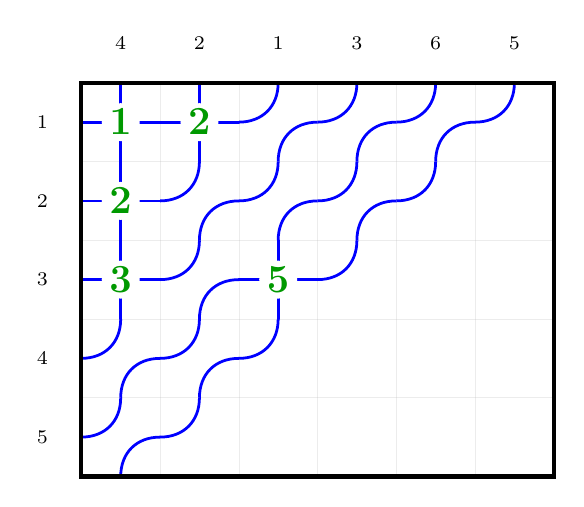
\begin{tikzpicture}[scale=1.0]
  \draw[lightgray, very thin, opacity=0.3] (0,1) -- (6,1);
  \draw[lightgray, very thin, opacity=0.3] (0,2) -- (6,2);
  \draw[lightgray, very thin, opacity=0.3] (0,3) -- (6,3);
  \draw[lightgray, very thin, opacity=0.3] (0,4) -- (6,4);
  \draw[lightgray, very thin, opacity=0.3] (0,5) -- (6,5);
  \draw[lightgray, very thin, opacity=0.3] (0,6) -- (6,6);
  \draw[lightgray, very thin, opacity=0.3] (0,1) -- (0,6);
  \draw[lightgray, very thin, opacity=0.3] (1,1) -- (1,6);
  \draw[lightgray, very thin, opacity=0.3] (2,1) -- (2,6);
  \draw[lightgray, very thin, opacity=0.3] (3,1) -- (3,6);
  \draw[lightgray, very thin, opacity=0.3] (4,1) -- (4,6);
  \draw[lightgray, very thin, opacity=0.3] (5,1) -- (5,6);
  \draw[lightgray, very thin, opacity=0.3] (6,1) -- (6,6);
  \draw[blue, line width=1.0pt, line cap=round] (0,5.5) -- (1,5.5);
  \draw[blue, line width=1.0pt, line cap=round] (0.5,5) -- (0.5,6);
  \draw[blue, line width=1.0pt, line cap=round] (1,5.5) -- (2,5.5);
  \draw[blue, line width=1.0pt, line cap=round] (1.5,5) -- (1.5,6);
  \draw[blue, line width=1.0pt] (2,5.5) .. controls (2.3,5.5) and (2.5,5.7) .. (2.5,6);
  \draw[blue, line width=1.0pt] (2.5,5) .. controls (2.5,5.3) and (2.7,5.5) .. (3,5.5);
  \draw[blue, line width=1.0pt] (3,5.5) .. controls (3.3,5.5) and (3.5,5.7) .. (3.5,6);
  \draw[blue, line width=1.0pt] (3.5,5) .. controls (3.5,5.3) and (3.7,5.5) .. (4,5.5);
  \draw[blue, line width=1.0pt] (4,5.5) .. controls (4.3,5.5) and (4.5,5.7) .. (4.5,6);
  \draw[blue, line width=1.0pt] (4.5,5) .. controls (4.5,5.3) and (4.7,5.5) .. (5,5.5);
  \draw[blue, line width=1.0pt] (5,5.5) .. controls (5.3,5.5) and (5.5,5.7) .. (5.5,6);
  \draw[blue, line width=1.0pt, line cap=round] (0,4.5) -- (1,4.5);
  \draw[blue, line width=1.0pt, line cap=round] (0.5,4) -- (0.5,5);
  \draw[blue, line width=1.0pt] (1,4.5) .. controls (1.3,4.5) and (1.5,4.7) .. (1.5,5);
  \draw[blue, line width=1.0pt] (1.5,4) .. controls (1.5,4.3) and (1.7,4.5) .. (2,4.5);
  \draw[blue, line width=1.0pt] (2,4.5) .. controls (2.3,4.5) and (2.5,4.7) .. (2.5,5);
  \draw[blue, line width=1.0pt] (2.5,4) .. controls (2.5,4.3) and (2.7,4.5) .. (3,4.5);
  \draw[blue, line width=1.0pt] (3,4.5) .. controls (3.3,4.5) and (3.5,4.7) .. (3.5,5);
  \draw[blue, line width=1.0pt] (3.5,4) .. controls (3.5,4.3) and (3.7,4.5) .. (4,4.5);
  \draw[blue, line width=1.0pt] (4,4.5) .. controls (4.3,4.5) and (4.5,4.7) .. (4.5,5);
  \draw[blue, line width=1.0pt, line cap=round] (0,3.5) -- (1,3.5);
  \draw[blue, line width=1.0pt, line cap=round] (0.5,3) -- (0.5,4);
  \draw[blue, line width=1.0pt] (1,3.5) .. controls (1.3,3.5) and (1.5,3.7) .. (1.5,4);
  \draw[blue, line width=1.0pt] (1.5,3) .. controls (1.5,3.3) and (1.7,3.5) .. (2,3.5);
  \draw[blue, line width=1.0pt, line cap=round] (2,3.5) -- (3,3.5);
  \draw[blue, line width=1.0pt, line cap=round] (2.5,3) -- (2.5,4);
  \draw[blue, line width=1.0pt] (3,3.5) .. controls (3.3,3.5) and (3.5,3.7) .. (3.5,4);
  \draw[blue, line width=1.0pt] (0,2.5) .. controls (0.3,2.5) and (0.5,2.7) .. (0.5,3);
  \draw[blue, line width=1.0pt] (0.5,2) .. controls (0.5,2.3) and (0.7,2.5) .. (1,2.5);
  \draw[blue, line width=1.0pt] (1,2.5) .. controls (1.3,2.5) and (1.5,2.7) .. (1.5,3);
  \draw[blue, line width=1.0pt] (1.5,2) .. controls (1.5,2.3) and (1.7,2.5) .. (2,2.5);
  \draw[blue, line width=1.0pt] (2,2.5) .. controls (2.3,2.5) and (2.5,2.7) .. (2.5,3);
  \draw[blue, line width=1.0pt] (0,1.5) .. controls (0.3,1.5) and (0.5,1.7) .. (0.5,2);
  \draw[blue, line width=1.0pt] (0.5,1) .. controls (0.5,1.3) and (0.7,1.5) .. (1,1.5);
  \draw[blue, line width=1.0pt] (1,1.5) .. controls (1.3,1.5) and (1.5,1.7) .. (1.5,2);
  \node[font=\Large\bfseries, text=green!60!black, fill=white, inner sep=0.5pt, circle, transform shape] at (1.5,5.5) {2};
  \node[font=\Large\bfseries, text=green!60!black, fill=white, inner sep=0.5pt, circle, transform shape] at (0.5,4.5) {2};
  \node[font=\Large\bfseries, text=green!60!black, fill=white, inner sep=0.5pt, circle, transform shape] at (0.5,3.5) {3};
  \node[font=\Large\bfseries, text=green!60!black, fill=white, inner sep=0.5pt, circle, transform shape] at (0.5,5.5) {1};
  \node[font=\Large\bfseries, text=green!60!black, fill=white, inner sep=0.5pt, circle, transform shape] at (2.5,3.5) {5};
  \node[font=\scriptsize, text=black, anchor=south] at (0.5,6.3) {4};
  \node[font=\scriptsize, text=black, anchor=south] at (1.5,6.3) {2};
  \node[font=\scriptsize, text=black, anchor=south] at (2.5,6.3) {1};
  \node[font=\scriptsize, text=black, anchor=south] at (3.5,6.3) {3};
  \node[font=\scriptsize, text=black, anchor=south] at (4.5,6.3) {6};
  \node[font=\scriptsize, text=black, anchor=south] at (5.5,6.3) {5};
  \node[font=\scriptsize, text=black, anchor=east] at (-0.3,5.5) {1};
  \node[font=\scriptsize, text=black, anchor=east] at (-0.3,4.5) {2};
  \node[font=\scriptsize, text=black, anchor=east] at (-0.3,3.5) {3};
  \node[font=\scriptsize, text=black, anchor=east] at (-0.3,2.5) {4};
  \node[font=\scriptsize, text=black, anchor=east] at (-0.3,1.5) {5};
  \draw[black, line width=1.5pt] (0,1) rectangle (6,6);
\end{tikzpicture}
\end{figure}


The main benefit of this is that visualizing $\rtt_R(i,j)$ is easy. The pipes that pass through position $(i,j)$ are labeled $s$ and $q$ for some $s,q>0$. For a positive root in an unoccupied square, we will have the following labeling, where $q<s$:

\begin{center}
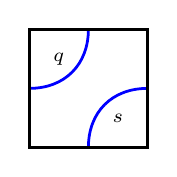
\begin{tikzpicture}[scale=1.5]
  % Draw the grid for a single square
  \draw[lightgray, very thin, opacity=0.3] (0,0) -- (1,0);
  \draw[lightgray, very thin, opacity=0.3] (0,1) -- (1,1);
  \draw[lightgray, very thin, opacity=0.3] (0,0) -- (0,1);
  \draw[lightgray, very thin, opacity=0.3] (1,0) -- (1,1);
  
  % Draw the elbow with two arcs
  % Blue arc (from left to top)
  \draw[blue, line width=1.0pt] (0,0.5) .. controls (0.3,0.5) and (0.5,0.7) .. (0.5,1);
  
  % Red arc (from bottom to right)
  \draw[blue, line width=1.0pt] (0.5,0) .. controls (0.5,0.3) and (0.7,0.5) .. (1,0.5);
  
  % Labels
  \node[font=\scriptsize, text=black] at (0.25,0.75) {$q$};
  \node[font=\scriptsize, text=black] at (0.75,0.25) {$s$};
  
  % Box around the grid
  \draw[black, line width=1.2pt] (0,0) rectangle (1,1);
\end{tikzpicture}
\end{center}

We observe that in the above RC graph, the position $(1,5)$ does not have this configuration. Placing a crossing there would create a negative root, and the pipes would cross twice. \emph{Note that this results in a collection of ordered pairs that is not an RC graph, if such a crossing exists.} For a valid RC graphs, only positive roots occur as crossings, and this happens if and only if pipes cross at most once.

\begin{figure}[h]
\centering
\caption{An invalid set of crossings causing pipes to cross more than once, caused by inserting a crossing at a negative root}
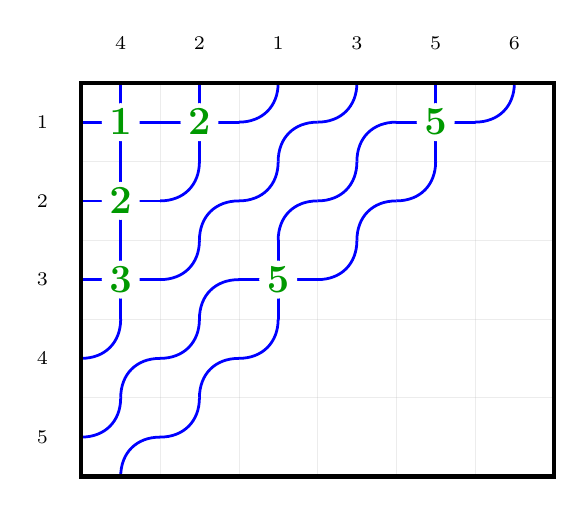
\begin{tikzpicture}[scale=1.0]
  \draw[lightgray, very thin, opacity=0.3] (0,1) -- (6,1);
  \draw[lightgray, very thin, opacity=0.3] (0,2) -- (6,2);
  \draw[lightgray, very thin, opacity=0.3] (0,3) -- (6,3);
  \draw[lightgray, very thin, opacity=0.3] (0,4) -- (6,4);
  \draw[lightgray, very thin, opacity=0.3] (0,5) -- (6,5);
  \draw[lightgray, very thin, opacity=0.3] (0,6) -- (6,6);
  \draw[lightgray, very thin, opacity=0.3] (0,1) -- (0,6);
  \draw[lightgray, very thin, opacity=0.3] (1,1) -- (1,6);
  \draw[lightgray, very thin, opacity=0.3] (2,1) -- (2,6);
  \draw[lightgray, very thin, opacity=0.3] (3,1) -- (3,6);
  \draw[lightgray, very thin, opacity=0.3] (4,1) -- (4,6);
  \draw[lightgray, very thin, opacity=0.3] (5,1) -- (5,6);
  \draw[lightgray, very thin, opacity=0.3] (6,1) -- (6,6);
  \draw[blue, line width=1.0pt, line cap=round] (0,5.5) -- (1,5.5);
  \draw[blue, line width=1.0pt, line cap=round] (0.5,5) -- (0.5,6);
  \draw[blue, line width=1.0pt, line cap=round] (1,5.5) -- (2,5.5);
  \draw[blue, line width=1.0pt, line cap=round] (1.5,5) -- (1.5,6);
  \draw[blue, line width=1.0pt] (2,5.5) .. controls (2.3,5.5) and (2.5,5.7) .. (2.5,6);
  \draw[blue, line width=1.0pt] (2.5,5) .. controls (2.5,5.3) and (2.7,5.5) .. (3,5.5);
  \draw[blue, line width=1.0pt] (3,5.5) .. controls (3.3,5.5) and (3.5,5.7) .. (3.5,6);
  \draw[blue, line width=1.0pt] (3.5,5) .. controls (3.5,5.3) and (3.7,5.5) .. (4,5.5);
  \draw[blue, line width=1.0pt, line cap=round] (4,5.5) -- (5,5.5);
  \draw[blue, line width=1.0pt, line cap=round] (4.5,5) -- (4.5,6);
  \draw[blue, line width=1.0pt] (5,5.5) .. controls (5.3,5.5) and (5.5,5.7) .. (5.5,6);
  \draw[blue, line width=1.0pt, line cap=round] (0,4.5) -- (1,4.5);
  \draw[blue, line width=1.0pt, line cap=round] (0.5,4) -- (0.5,5);
  \draw[blue, line width=1.0pt] (1,4.5) .. controls (1.3,4.5) and (1.5,4.7) .. (1.5,5);
  \draw[blue, line width=1.0pt] (1.5,4) .. controls (1.5,4.3) and (1.7,4.5) .. (2,4.5);
  \draw[blue, line width=1.0pt] (2,4.5) .. controls (2.3,4.5) and (2.5,4.7) .. (2.5,5);
  \draw[blue, line width=1.0pt] (2.5,4) .. controls (2.5,4.3) and (2.7,4.5) .. (3,4.5);
  \draw[blue, line width=1.0pt] (3,4.5) .. controls (3.3,4.5) and (3.5,4.7) .. (3.5,5);
  \draw[blue, line width=1.0pt] (3.5,4) .. controls (3.5,4.3) and (3.7,4.5) .. (4,4.5);
  \draw[blue, line width=1.0pt] (4,4.5) .. controls (4.3,4.5) and (4.5,4.7) .. (4.5,5);
  \draw[blue, line width=1.0pt, line cap=round] (0,3.5) -- (1,3.5);
  \draw[blue, line width=1.0pt, line cap=round] (0.5,3) -- (0.5,4);
  \draw[blue, line width=1.0pt] (1,3.5) .. controls (1.3,3.5) and (1.5,3.7) .. (1.5,4);
  \draw[blue, line width=1.0pt] (1.5,3) .. controls (1.5,3.3) and (1.7,3.5) .. (2,3.5);
  \draw[blue, line width=1.0pt, line cap=round] (2,3.5) -- (3,3.5);
  \draw[blue, line width=1.0pt, line cap=round] (2.5,3) -- (2.5,4);
  \draw[blue, line width=1.0pt] (3,3.5) .. controls (3.3,3.5) and (3.5,3.7) .. (3.5,4);
  \draw[blue, line width=1.0pt] (0,2.5) .. controls (0.3,2.5) and (0.5,2.7) .. (0.5,3);
  \draw[blue, line width=1.0pt] (0.5,2) .. controls (0.5,2.3) and (0.7,2.5) .. (1,2.5);
  \draw[blue, line width=1.0pt] (1,2.5) .. controls (1.3,2.5) and (1.5,2.7) .. (1.5,3);
  \draw[blue, line width=1.0pt] (1.5,2) .. controls (1.5,2.3) and (1.7,2.5) .. (2,2.5);
  \draw[blue, line width=1.0pt] (2,2.5) .. controls (2.3,2.5) and (2.5,2.7) .. (2.5,3);
  \draw[blue, line width=1.0pt] (0,1.5) .. controls (0.3,1.5) and (0.5,1.7) .. (0.5,2);
  \draw[blue, line width=1.0pt] (0.5,1) .. controls (0.5,1.3) and (0.7,1.5) .. (1,1.5);
  \draw[blue, line width=1.0pt] (1,1.5) .. controls (1.3,1.5) and (1.5,1.7) .. (1.5,2);
  \node[font=\Large\bfseries, text=green!60!black, fill=white, inner sep=0.5pt, circle, transform shape] at (1.5,5.5) {2};
  \node[font=\Large\bfseries, text=green!60!black, fill=white, inner sep=0.5pt, circle, transform shape] at (0.5,4.5) {2};
  \node[font=\Large\bfseries, text=green!60!black, fill=white, inner sep=0.5pt, circle, transform shape] at (4.5,5.5) {5};
  \node[font=\Large\bfseries, text=green!60!black, fill=white, inner sep=0.5pt, circle, transform shape] at (0.5,3.5) {3};
  \node[font=\Large\bfseries, text=green!60!black, fill=white, inner sep=0.5pt, circle, transform shape] at (0.5,5.5) {1};
  \node[font=\Large\bfseries, text=green!60!black, fill=white, inner sep=0.5pt, circle, transform shape] at (2.5,3.5) {5};
  \node[font=\scriptsize, text=black, anchor=south] at (0.5,6.3) {4};
  \node[font=\scriptsize, text=black, anchor=south] at (1.5,6.3) {2};
  \node[font=\scriptsize, text=black, anchor=south] at (2.5,6.3) {1};
  \node[font=\scriptsize, text=black, anchor=south] at (3.5,6.3) {3};
  \node[font=\scriptsize, text=black, anchor=south] at (4.5,6.3) {5};
  \node[font=\scriptsize, text=black, anchor=south] at (5.5,6.3) {6};
  \node[font=\scriptsize, text=black, anchor=east] at (-0.3,5.5) {1};
  \node[font=\scriptsize, text=black, anchor=east] at (-0.3,4.5) {2};
  \node[font=\scriptsize, text=black, anchor=east] at (-0.3,3.5) {3};
  \node[font=\scriptsize, text=black, anchor=east] at (-0.3,2.5) {4};
  \node[font=\scriptsize, text=black, anchor=east] at (-0.3,1.5) {5};
  \draw[black, line width=1.5pt] (0,1) rectangle (6,6);
\end{tikzpicture}
\end{figure}

\subsection{Zeroing out the last row}

We proceed now to define a product on $\BRC$ turning it into a ring. To do this, we need to be able to define a function $\zeromap:\BRC\to\BRC$ trimming empty rows from the bottom instead of from the top. This is far more complicated.


\newcommand{\xleadsto}[2][]{\overset{#2}{\leadsto}}

\newcommand{\ins}[2]{{#2\xleadsto{#1}}}

\begin{algorithm}
\caption{Basic monk insertion $\ins{k}{i} R$}
\label{algorithm:monk}
\begin{algorithmic}[1]
		\State \textbf{Input:} An RC graph $R$, parameter $k$, and an integer $i$ with $1\leq i\leq k$.
		\State \textbf{Output:} A modified RC graph $R'$ with $\wtt_j(R')=\wtt_j(R)$  for $j\neq i$ and $\wtt_i(R')=\wtt_i(R)+1$ such that $\wof{R}\tom{k} \wof{R'}$.
		\State Find leftmost position $(i, j) \notin R$ in row $i$ such that if $\rtt_R(i, j)=(a,b)$, then $a\leq k < b$.
		\State $R \gets R \cup \{(i, j)\}$
    \If{there exists $(i', j') \in R$ with $\rtt_R(i', j') \in \Phi^-$}
        \State $R \gets R \setminus \{(i', j')\}$
        \State Return to step 3 substituting $i = i'$.
    \EndIf
		\State \Return $R$
	\end{algorithmic}
\end{algorithm}

\begin{algorithm} 
	\caption{Pseudo-Pieri insertion $\ins{k}{I} R$}
	\label{algorithm:insertion}
	\begin{algorithmic}[1]
		\State \textbf{Input:} An RC graph $R$, parameter $k$, and sequence $I = \{i_1, \ldots, i_m\}$ with $k\geq i_1 \geq i_2 \geq \cdots \geq i_m \geq 1$.
		\State \textbf{Output:} A modified RC graph $R'$ with $\wtt_i(R')=\wtt_i(R)$ for $i\notin I$ and $\wtt_i(R')=\wtt_i(R)+\#\{j \mid i_j = i\}$ for $i\in I$ such that $\wof{R}\Tom{k} \wof{R'}$.
		\State \textbf{Initialize:} Let $L \gets [\,]$ (empty list of pairs $(a, b)$ where $a \leq k < b$), and $U\gets [\,]$ (empty list of positions).
		\For{each $i \in (i_1, \ldots, i_m)$}
		\State Find leftmost position $(i, j) \notin R$ in row $i$ satisfying $j>j'$ for all $(i,j')\in U$ such that either:
		\State \quad a) $\rtt_R(i, j) = (s, q)$ where $s \leq k < q$ and $q \notin \{b \mid (a, b) \in L\}$.
		\State \quad b) $\rtt_R(i, j) = (b_r, q)$ where $q > k$, $b_r<q$, and $q \notin \{b \mid (a, b) \in L\}$.
		\State $R \gets R \cup \{(i, j)\}$ and $U\gets U \cup \{(i, j)\}$
		\State Update $L$ by adding $(s, q)$ or replacing $(a_r, b_r)$ with $(a_r, q)$ and $(a_r, b_r)$.
		\If{there exists $(i', j') \in R$ with $\rtt_R(i', j') \in \Phi^-$}
        
    \State $R \gets R \setminus \{(i', j')\}$
		\State Let $\rtt_R(i', j') = (q, s)$
		\If{$(s, q) \in L$}
		\State Remove $(s, q)$ from $L$
		\Else
		\State Remove $(a_r, q)$ from $L$, where $(a_r, q),(a_r,s)\in L$
		\EndIf
		\State Return to step 5 to insert $i'$.
    \EndIf
		\EndFor
		\State \Return $R$
	\end{algorithmic}
\end{algorithm}


\begin{algorithm}
	\caption{Map $\zeromap(R)$ zeroing out last row}
	\label{algorithm:zero}
	\begin{algorithmic}[1]
		\State \textbf{Input:} A bounded RC graph $R$ with $\hr(R)=n$ and row $n$ empty.
		\State \textbf{Output:} A bounded RC graph $R'$ with $\hr(R')=n-1$, $|R'|=|R|$ (same number of crossings), and $\wof{R}\downvar{n} \wof{R'}$.
		
		\If{$R$ with last row removed is a valid bounded RC graph}
		\State \Return $R$ with last row removed
		\Else
		\State Let $R_0 \gets R$.
		\State Find the maximal $p$ and sequence $\{(i_m, j_m)\}_{m=1}^p$ such that:
		\State \quad $\rtt_{R_{m-1}}(i_m, j_m) = (n+m-1,n+m)$ for each $m$, where $R_m = R_{m-1}\setminus\{(i_m, j_m)\}$ for each $m\geq 1$.
		\State $R^- \gets R \setminus \{(i_1, j_1), \ldots, (i_p, j_p)\}$.
		\State Let $I \gets (i_1, i_2, \ldots, i_p)$.
		\State $D \gets R^- \cup \{(n, 1), (n, 2), \ldots, (n, p)\}$.
		\State $D' \gets \ins{n-1}{I} D$
		\State $R' \gets \{(i, j) \in D' \mid i < n\}$ as a bounded RC graph with $n-1$ rows.
		\State \Return $R'$.
		\EndIf
	\end{algorithmic}
\end{algorithm}

See Figure \ref{fig:zeroing} for an example of the zeroing operation (Algorithm \ref{algorithm:zero}). 

\def\multiset#1#2{\ensuremath{\left(\kern-.3em\left(\genfrac{}{}{0pt}{}{#1}{#2}\right)\kern-.3em\right)}}


Note that Algorithm \ref{algorithm:insertion} is \emph{not} a realization of Sottile's Pieri formula for complete symmetric polynomials, despite preserving the relevant Bruhat relation. This is because the map 
$$\multiset{k}{p}\times\RC(w)\to \RC(n)$$
given by 
$$(I, R)\mapsto \ins{k}{I} R$$ 
need not be injective.


\begin{figure}[htbp]
\centering

% First diagram
\begin{minipage}{0.45\textwidth}
\centering
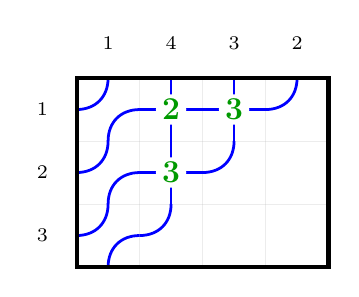
\begin{tikzpicture}[scale=0.8]
  \draw[lightgray, very thin, opacity=0.3] (0,1) -- (4,1);
  \draw[lightgray, very thin, opacity=0.3] (0,2) -- (4,2);
  \draw[lightgray, very thin, opacity=0.3] (0,3) -- (4,3);
  \draw[lightgray, very thin, opacity=0.3] (0,4) -- (4,4);
  \draw[lightgray, very thin, opacity=0.3] (0,1) -- (0,4);
  \draw[lightgray, very thin, opacity=0.3] (1,1) -- (1,4);
  \draw[lightgray, very thin, opacity=0.3] (2,1) -- (2,4);
  \draw[lightgray, very thin, opacity=0.3] (3,1) -- (3,4);
  \draw[lightgray, very thin, opacity=0.3] (4,1) -- (4,4);
  \draw[blue, line width=1.0pt] (0,3.5) .. controls (0.3,3.5) and (0.5,3.7) .. (0.5,4);
  \draw[blue, line width=1.0pt] (0.5,3) .. controls (0.5,3.3) and (0.7,3.5) .. (1,3.5);
  \draw[blue, line width=1.0pt, line cap=round] (1,3.5) -- (2,3.5);
  \draw[blue, line width=1.0pt, line cap=round] (1.5,3) -- (1.5,4);
  \draw[blue, line width=1.0pt, line cap=round] (2,3.5) -- (3,3.5);
  \draw[blue, line width=1.0pt, line cap=round] (2.5,3) -- (2.5,4);
  \draw[blue, line width=1.0pt] (3,3.5) .. controls (3.3,3.5) and (3.5,3.7) .. (3.5,4);
  \draw[blue, line width=1.0pt] (0,2.5) .. controls (0.3,2.5) and (0.5,2.7) .. (0.5,3);
  \draw[blue, line width=1.0pt] (0.5,2) .. controls (0.5,2.3) and (0.7,2.5) .. (1,2.5);
  \draw[blue, line width=1.0pt, line cap=round] (1,2.5) -- (2,2.5);
  \draw[blue, line width=1.0pt, line cap=round] (1.5,2) -- (1.5,3);
  \draw[blue, line width=1.0pt] (2,2.5) .. controls (2.3,2.5) and (2.5,2.7) .. (2.5,3);
  \draw[blue, line width=1.0pt] (0,1.5) .. controls (0.3,1.5) and (0.5,1.7) .. (0.5,2);
  \draw[blue, line width=1.0pt] (0.5,1) .. controls (0.5,1.3) and (0.7,1.5) .. (1,1.5);
  \draw[blue, line width=1.0pt] (1,1.5) .. controls (1.3,1.5) and (1.5,1.7) .. (1.5,2);
  \node[font=\Large\bfseries, text=green!60!black, fill=white, inner sep=0.5pt, circle, transform shape] at (1.5,3.5) {2};
  \node[font=\Large\bfseries, text=green!60!black, fill=white, inner sep=0.5pt, circle, transform shape] at (2.5,3.5) {3};
  \node[font=\Large\bfseries, text=green!60!black, fill=white, inner sep=0.5pt, circle, transform shape] at (1.5,2.5) {3};
  \node[font=\scriptsize, text=black, anchor=south] at (0.5,4.3) {1};
  \node[font=\scriptsize, text=black, anchor=south] at (1.5,4.3) {4};
  \node[font=\scriptsize, text=black, anchor=south] at (2.5,4.3) {3};
  \node[font=\scriptsize, text=black, anchor=south] at (3.5,4.3) {2};
  \node[font=\scriptsize, text=black, anchor=east] at (-0.3,3.5) {1};
  \node[font=\scriptsize, text=black, anchor=east] at (-0.3,2.5) {2};
  \node[font=\scriptsize, text=black, anchor=east] at (-0.3,1.5) {3};
  \draw[black, line width=1.5pt] (0,1) rectangle (4,4);
\end{tikzpicture}
\caption*{(a) Initial RC graph $R$}
\end{minipage}
\hfill
% Second diagram
\begin{minipage}{0.45\textwidth}
\centering
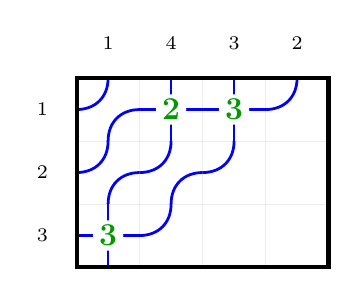
\begin{tikzpicture}[scale=0.8]
  \draw[lightgray, very thin, opacity=0.3] (0,1) -- (4,1);
  \draw[lightgray, very thin, opacity=0.3] (0,2) -- (4,2);
  \draw[lightgray, very thin, opacity=0.3] (0,3) -- (4,3);
  \draw[lightgray, very thin, opacity=0.3] (0,4) -- (4,4);
  \draw[lightgray, very thin, opacity=0.3] (0,1) -- (0,4);
  \draw[lightgray, very thin, opacity=0.3] (1,1) -- (1,4);
  \draw[lightgray, very thin, opacity=0.3] (2,1) -- (2,4);
  \draw[lightgray, very thin, opacity=0.3] (3,1) -- (3,4);
  \draw[lightgray, very thin, opacity=0.3] (4,1) -- (4,4);
  \draw[blue, line width=1.0pt] (0,3.5) .. controls (0.3,3.5) and (0.5,3.7) .. (0.5,4);
  \draw[blue, line width=1.0pt] (0.5,3) .. controls (0.5,3.3) and (0.7,3.5) .. (1,3.5);
  \draw[blue, line width=1.0pt, line cap=round] (1,3.5) -- (2,3.5);
  \draw[blue, line width=1.0pt, line cap=round] (1.5,3) -- (1.5,4);
  \draw[blue, line width=1.0pt, line cap=round] (2,3.5) -- (3,3.5);
  \draw[blue, line width=1.0pt, line cap=round] (2.5,3) -- (2.5,4);
  \draw[blue, line width=1.0pt] (3,3.5) .. controls (3.3,3.5) and (3.5,3.7) .. (3.5,4);
  \draw[blue, line width=1.0pt] (0,2.5) .. controls (0.3,2.5) and (0.5,2.7) .. (0.5,3);
  \draw[blue, line width=1.0pt] (0.5,2) .. controls (0.5,2.3) and (0.7,2.5) .. (1,2.5);
  \draw[blue, line width=1.0pt] (1,2.5) .. controls (1.3,2.5) and (1.5,2.7) .. (1.5,3);
  \draw[blue, line width=1.0pt] (1.5,2) .. controls (1.5,2.3) and (1.7,2.5) .. (2,2.5);
  \draw[blue, line width=1.0pt] (2,2.5) .. controls (2.3,2.5) and (2.5,2.7) .. (2.5,3);
  \draw[blue, line width=1.0pt, line cap=round] (0,1.5) -- (1,1.5);
  \draw[blue, line width=1.0pt, line cap=round] (0.5,1) -- (0.5,2);
  \draw[blue, line width=1.0pt] (1,1.5) .. controls (1.3,1.5) and (1.5,1.7) .. (1.5,2);
  \node[font=\Large\bfseries, text=green!60!black, fill=white, inner sep=0.5pt, circle, transform shape] at (0.5,1.5) {3};
  \node[font=\Large\bfseries, text=green!60!black, fill=white, inner sep=0.5pt, circle, transform shape] at (1.5,3.5) {2};
  \node[font=\Large\bfseries, text=green!60!black, fill=white, inner sep=0.5pt, circle, transform shape] at (2.5,3.5) {3};
  \node[font=\scriptsize, text=black, anchor=south] at (0.5,4.3) {1};
  \node[font=\scriptsize, text=black, anchor=south] at (1.5,4.3) {4};
  \node[font=\scriptsize, text=black, anchor=south] at (2.5,4.3) {3};
  \node[font=\scriptsize, text=black, anchor=south] at (3.5,4.3) {2};
  \node[font=\scriptsize, text=black, anchor=east] at (-0.3,3.5) {1};
  \node[font=\scriptsize, text=black, anchor=east] at (-0.3,2.5) {2};
  \node[font=\scriptsize, text=black, anchor=east] at (-0.3,1.5) {3};
  \draw[black, line width=1.5pt] (0,1) rectangle (4,4);
\end{tikzpicture}
\caption*{(b) After deleting $(2,2)$ with $\rtt_R(2,2)=\alpha_3$ and moving to row $3$}
\end{minipage}

\vspace{1em}

% Third diagram
\begin{minipage}{0.45\textwidth}
\centering
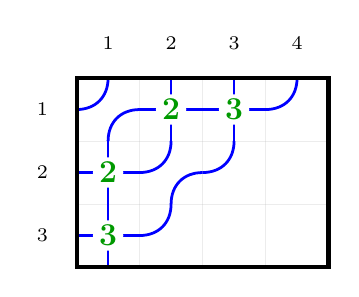
\begin{tikzpicture}[scale=0.8]
  \draw[lightgray, very thin, opacity=0.3] (0,1) -- (4,1);
  \draw[lightgray, very thin, opacity=0.3] (0,2) -- (4,2);
  \draw[lightgray, very thin, opacity=0.3] (0,3) -- (4,3);
  \draw[lightgray, very thin, opacity=0.3] (0,4) -- (4,4);
  \draw[lightgray, very thin, opacity=0.3] (0,1) -- (0,4);
  \draw[lightgray, very thin, opacity=0.3] (1,1) -- (1,4);
  \draw[lightgray, very thin, opacity=0.3] (2,1) -- (2,4);
  \draw[lightgray, very thin, opacity=0.3] (3,1) -- (3,4);
  \draw[lightgray, very thin, opacity=0.3] (4,1) -- (4,4);
  \draw[blue, line width=1.0pt] (0,3.5) .. controls (0.3,3.5) and (0.5,3.7) .. (0.5,4);
  \draw[blue, line width=1.0pt] (0.5,3) .. controls (0.5,3.3) and (0.7,3.5) .. (1,3.5);
  \draw[blue, line width=1.0pt, line cap=round] (1,3.5) -- (2,3.5);
  \draw[blue, line width=1.0pt, line cap=round] (1.5,3) -- (1.5,4);
  \draw[blue, line width=1.0pt, line cap=round] (2,3.5) -- (3,3.5);
  \draw[blue, line width=1.0pt, line cap=round] (2.5,3) -- (2.5,4);
  \draw[blue, line width=1.0pt] (3,3.5) .. controls (3.3,3.5) and (3.5,3.7) .. (3.5,4);
  \draw[blue, line width=1.0pt, line cap=round] (0,2.5) -- (1,2.5);
  \draw[blue, line width=1.0pt, line cap=round] (0.5,2) -- (0.5,3);
  \draw[blue, line width=1.0pt] (1,2.5) .. controls (1.3,2.5) and (1.5,2.7) .. (1.5,3);
  \draw[blue, line width=1.0pt] (1.5,2) .. controls (1.5,2.3) and (1.7,2.5) .. (2,2.5);
  \draw[blue, line width=1.0pt] (2,2.5) .. controls (2.3,2.5) and (2.5,2.7) .. (2.5,3);
  \draw[blue, line width=1.0pt, line cap=round] (0,1.5) -- (1,1.5);
  \draw[blue, line width=1.0pt, line cap=round] (0.5,1) -- (0.5,2);
  \draw[blue, line width=1.0pt] (1,1.5) .. controls (1.3,1.5) and (1.5,1.7) .. (1.5,2);
  \node[font=\Large\bfseries, text=green!60!black, fill=white, inner sep=0.5pt, circle, transform shape] at (0.5,1.5) {3};
  \node[font=\Large\bfseries, text=green!60!black, fill=white, inner sep=0.5pt, circle, transform shape] at (1.5,3.5) {2};
  \node[font=\Large\bfseries, text=green!60!black, fill=white, inner sep=0.5pt, circle, transform shape] at (2.5,3.5) {3};
  \node[font=\Large\bfseries, text=green!60!black, fill=white, inner sep=0.5pt, circle, transform shape] at (0.5,2.5) {2};
  \node[font=\scriptsize, text=black, anchor=south] at (0.5,4.3) {1};
  \node[font=\scriptsize, text=black, anchor=south] at (1.5,4.3) {2};
  \node[font=\scriptsize, text=black, anchor=south] at (2.5,4.3) {3};
  \node[font=\scriptsize, text=black, anchor=south] at (3.5,4.3) {4};
  \node[font=\scriptsize, text=black, anchor=east] at (-0.3,3.5) {1};
  \node[font=\scriptsize, text=black, anchor=east] at (-0.3,2.5) {2};
  \node[font=\scriptsize, text=black, anchor=east] at (-0.3,1.5) {3};
  \draw[black, line width=1.5pt] (0,1) rectangle (4,4);
\end{tikzpicture}
\caption*{(c) After insertion with $i_1=2$}
\end{minipage}
\hfill
% Fourth diagram
\begin{minipage}{0.45\textwidth}
\centering
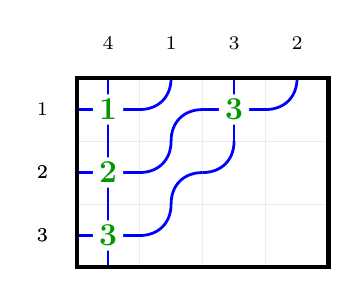
\begin{tikzpicture}[scale=0.8]
  \draw[lightgray, very thin, opacity=0.3] (0,1) -- (4,1);
  \draw[lightgray, very thin, opacity=0.3] (0,2) -- (4,2);
  \draw[lightgray, very thin, opacity=0.3] (0,3) -- (4,3);
  \draw[lightgray, very thin, opacity=0.3] (0,4) -- (4,4);
  \draw[lightgray, very thin, opacity=0.3] (0,1) -- (0,4);
  \draw[lightgray, very thin, opacity=0.3] (1,1) -- (1,4);
  \draw[lightgray, very thin, opacity=0.3] (2,1) -- (2,4);
  \draw[lightgray, very thin, opacity=0.3] (3,1) -- (3,4);
  \draw[lightgray, very thin, opacity=0.3] (4,1) -- (4,4);
  \draw[blue, line width=1.0pt, line cap=round] (0,3.5) -- (1,3.5);
  \draw[blue, line width=1.0pt, line cap=round] (0.5,3) -- (0.5,4);
  \draw[blue, line width=1.0pt] (1,3.5) .. controls (1.3,3.5) and (1.5,3.7) .. (1.5,4);
  \draw[blue, line width=1.0pt] (1.5,3) .. controls (1.5,3.3) and (1.7,3.5) .. (2,3.5);
  \draw[blue, line width=1.0pt, line cap=round] (2,3.5) -- (3,3.5);
  \draw[blue, line width=1.0pt, line cap=round] (2.5,3) -- (2.5,4);
  \draw[blue, line width=1.0pt] (3,3.5) .. controls (3.3,3.5) and (3.5,3.7) .. (3.5,4);
  \draw[blue, line width=1.0pt, line cap=round] (0,2.5) -- (1,2.5);
  \draw[blue, line width=1.0pt, line cap=round] (0.5,2) -- (0.5,3);
  \draw[blue, line width=1.0pt] (1,2.5) .. controls (1.3,2.5) and (1.5,2.7) .. (1.5,3);
  \draw[blue, line width=1.0pt] (1.5,2) .. controls (1.5,2.3) and (1.7,2.5) .. (2,2.5);
  \draw[blue, line width=1.0pt] (2,2.5) .. controls (2.3,2.5) and (2.5,2.7) .. (2.5,3);
  \draw[blue, line width=1.0pt, line cap=round] (0,1.5) -- (1,1.5);
  \draw[blue, line width=1.0pt, line cap=round] (0.5,1) -- (0.5,2);
  \draw[blue, line width=1.0pt] (1,1.5) .. controls (1.3,1.5) and (1.5,1.7) .. (1.5,2);
  \node[font=\Large\bfseries, text=green!60!black, fill=white, inner sep=0.5pt, circle, transform shape] at (0.5,1.5) {3};
  \node[font=\Large\bfseries, text=green!60!black, fill=white, inner sep=0.5pt, circle, transform shape] at (0.5,3.5) {1};
  \node[font=\Large\bfseries, text=green!60!black, fill=white, inner sep=0.5pt, circle, transform shape] at (2.5,3.5) {3};
  \node[font=\Large\bfseries, text=green!60!black, fill=white, inner sep=0.5pt, circle, transform shape] at (0.5,2.5) {2};
  \node[font=\scriptsize, text=black, anchor=south] at (0.5,4.3) {4};
  \node[font=\scriptsize, text=black, anchor=south] at (1.5,4.3) {1};
  \node[font=\scriptsize, text=black, anchor=south] at (2.5,4.3) {3};
  \node[font=\scriptsize, text=black, anchor=south] at (3.5,4.3) {2};
  \node[font=\scriptsize, text=black, anchor=east] at (-0.3,3.5) {1};
  \node[font=\scriptsize, text=black, anchor=east] at (-0.3,2.5) {2};
  \node[font=\scriptsize, text=black, anchor=east] at (-0.3,1.5) {3};
  \node[font=\scriptsize, text=black, anchor=east] at (-0.3,2.5) {2};
  \node[font=\scriptsize, text=black, anchor=east] at (-0.3,1.5) {3};
  \draw[black, line width=1.5pt] (0,1) rectangle (4,4);
\end{tikzpicture}
\caption*{(d) After rectification}
\end{minipage}

\vspace{1em}

% Fifth diagram
\begin{minipage}{0.45\textwidth}
\centering
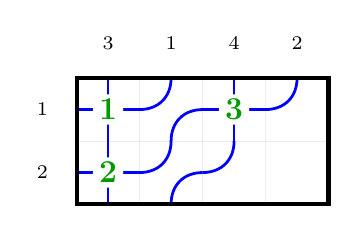
\begin{tikzpicture}[scale=0.8]
  \draw[lightgray, very thin, opacity=0.3] (0,2) -- (4,2);
  \draw[lightgray, very thin, opacity=0.3] (0,3) -- (4,3);
  \draw[lightgray, very thin, opacity=0.3] (0,4) -- (4,4);
  \draw[lightgray, very thin, opacity=0.3] (0,2) -- (0,4);
  \draw[lightgray, very thin, opacity=0.3] (1,2) -- (1,4);
  \draw[lightgray, very thin, opacity=0.3] (2,2) -- (2,4);
  \draw[lightgray, very thin, opacity=0.3] (3,2) -- (3,4);
  \draw[lightgray, very thin, opacity=0.3] (4,2) -- (4,4);
  \draw[blue, line width=1.0pt, line cap=round] (0,3.5) -- (1,3.5);
  \draw[blue, line width=1.0pt, line cap=round] (0.5,3) -- (0.5,4);
  \draw[blue, line width=1.0pt] (1,3.5) .. controls (1.3,3.5) and (1.5,3.7) .. (1.5,4);
  \draw[blue, line width=1.0pt] (1.5,3) .. controls (1.5,3.3) and (1.7,3.5) .. (2,3.5);
  \draw[blue, line width=1.0pt, line cap=round] (2,3.5) -- (3,3.5);
  \draw[blue, line width=1.0pt, line cap=round] (2.5,3) -- (2.5,4);
  \draw[blue, line width=1.0pt] (3,3.5) .. controls (3.3,3.5) and (3.5,3.7) .. (3.5,4);
  \draw[blue, line width=1.0pt, line cap=round] (0,2.5) -- (1,2.5);
  \draw[blue, line width=1.0pt, line cap=round] (0.5,2) -- (0.5,3);
  \draw[blue, line width=1.0pt] (1,2.5) .. controls (1.3,2.5) and (1.5,2.7) .. (1.5,3);
  \draw[blue, line width=1.0pt] (1.5,2) .. controls (1.5,2.3) and (1.7,2.5) .. (2,2.5);
  \draw[blue, line width=1.0pt] (2,2.5) .. controls (2.3,2.5) and (2.5,2.7) .. (2.5,3);
  \node[font=\Large\bfseries, text=green!60!black, fill=white, inner sep=0.5pt, circle, transform shape] at (0.5,3.5) {1};
  \node[font=\Large\bfseries, text=green!60!black, fill=white, inner sep=0.5pt, circle, transform shape] at (2.5,3.5) {3};
  \node[font=\Large\bfseries, text=green!60!black, fill=white, inner sep=0.5pt, circle, transform shape] at (0.5,2.5) {2};
  \node[font=\scriptsize, text=black, anchor=south] at (0.5,4.3) {3};
  \node[font=\scriptsize, text=black, anchor=south] at (1.5,4.3) {1};
  \node[font=\scriptsize, text=black, anchor=south] at (2.5,4.3) {4};
  \node[font=\scriptsize, text=black, anchor=south] at (3.5,4.3) {2};
  \node[font=\scriptsize, text=black, anchor=east] at (-0.3,3.5) {1};
  \node[font=\scriptsize, text=black, anchor=east] at (-0.3,2.5) {2};
  \draw[black, line width=1.5pt] (0,2) rectangle (4,4);
\end{tikzpicture}
\caption*{(e) Final result $\zeromap(R)=(R',2)$ after removing row 3}
\end{minipage}

\caption{Step-by-step computation of $\zeromap(R)$ for $R=\{(1,2),(1,3),(2,2)\}$.}
\label{fig:zeroing}
\end{figure}



\begin{lemma} \label{lemma:insertworks}
Given an RC graph $R$, an integer $k$, and $k\geq i_1\geq\cdots\geq i_m\geq 1$, Algorithm \ref{algorithm:insertion} produces a valid RC graph $R'$ satisfying
$$\wtt_i(R') = \wtt_i(R) + \#\{j \mid i_j = i\}$$
and
$$\wof{R}\Tom{k} \wof{R'}$$
\end{lemma}
\begin{proof}
Set $R_0=R$ to be the initial RC graph. We claim that given $R$ and $L$ at the start of iteration $p$ of the main loop, we have that $R$ is a valid RC graph satisfying
$$\wtt_i(R) = \wtt_i(R_0) + \#\{j \leq p-1 \mid i_j = i\}$$
and
$$\wof{R} = \wof{R_0}t_{a_1b_1}\cdots t_{a_{p-1}b_{p-1}}$$
where $L=[(a_1,b_1),\ldots,(a_p,b_p)]$. This is clear for $p=1$. For larger $p$, suppose we are inserting at row $i_p$. If we are in case (a) of Step 5, then adding $(i_p,j)$ to $R$ adds the root $t_s - t_q$ to the inversion set of $\wof{R}$, and multiplying by $t_{sq}$ gives the desired result. If we are in case (b) of Step 5, then adding $(i_p,j)$ to $R$ results in multiplication by $t_{b_rq}$. This commutes past the other reflections to meet $t_{a_rb_r}$. We thus have the situation
$$t_{a_rb_r}t_{b_rq} = t_{a_rq}t_{a_rb_r}$$
This ensures that the product remains as desired if the RC graph is valid. However, the condition that the RC graph $R$ be valid is not guaranteed after this step, so we must rectify. Suppose we must rectify at row $i - 1$. We find a negative root $(i-1, j')$ which must have been created by the insertion, and hence by the strong exchange property equal to $\rtt_R(i, j)$ that was inserted. Removing this root (from both the graph and from $L$) returns us to the original permutation at the beginning of the iteration, and performing the insert at row $i-1$ adds a new positive root, giving the desired result on the permutation. The weight is unchanged since we removed and added one crossing in row $i-1$. If the algorithm ends here, we have instead multiplied by the new reflection obtained in the ultimate insert step. Otherwise, repeating this process for all necessary rectifications completes the proof of the claim. The claim iterated to $p=m+1$ yields the desired result, and the method of updating $L$ ensures that the $b_j$ are all distinct, so that $\wof{R}\Tom{k} \wof{R'}$.
\end{proof}


\begin{lemma}
Given a bounded RC graph $R$ with $\hr(R)=n$ such that row $n$ is empty, Algorithm \ref{algorithm:zero} produces a valid bounded RC graph $R'$ with $\hr(R')=n-1$ satisfying
$$\wtt(R') = \wtt(R)$$
\end{lemma}
\begin{proof}
	Stripping out the crossings at roots $(n, n+1), (n+1, n+2), \ldots, (n + p - 1, n + p)$ removes exactly one crossing from each of rows $i_1, i_2, \ldots, i_p$, and moving them to the last row to obtain $R_1$ ensures that $\wof{R}=\wof{R_1}$. By construction, the portion of the RC graph in rows with index less than $n$ is valid (meaning its max descent is at most $n-1$). Applying Algorithm \ref{algorithm:insertion} to insert at rows $i_1, i_2, \ldots, i_p$ adds different crossings to preserve the number of elements in each row without adding descents past index $n$ in the permutation, by Lemma \ref{lemma:insertworks}. Removing row $n$ then yields a valid bounded RC graph $R'$ with $|R'|=n-1$ and the desired properties. 
\end{proof}



\begin{theorem} \label{theorem:zero_bijection}
Let $w$ be a permutation with last descent at most $n$. Let $\mathcal{RC}(w,n)^0$ be the set of bounded RC graphs $R$ with $\hr(R)=n$ such that $\wof{R}=w$ and row $n$ is empty. Then
$$\zeromap:\mathcal{RC}(w, n)^{0}\to \bigcup_{w\downvar{n} w'}\mathcal{RC}(w', n-1)$$
is a weight-preserving bijection.
\end{theorem}

To prove Theorem \ref{theorem:zero_bijection} for $n=2$, we may characterize the bounded RC graphs $R$ with $|R|=2$ such that row $2$ is empty and $\maxd(\wof{R})=2$ as those for permutations $w=s_k s_{k-1}\cdots s_2$ for some $k>1$. Algorithm \ref{algorithm:zero} in this case consists moves the entirety of the crossings in row $1$ to row $2$. The procedure then inserts $k-1$ crossings into row $1$ in order from left to right, which must have roots $t_q - t_s$ such that $q=1$. Thus $R'$ is precisely $\{(1,1), (1,2), (1,3), \ldots, (1, k-1)\}$, which is the unique bounded RC graph for the permutation $w' = s_{k-1} s_{k-2}\cdots s_1$ with one row. This establishes the base case.

For the induction step, we require the following lemmas.

\begin{lemma} \label{lemma:zerotransition}
Let $R$ be a bounded RC graph with $\hr(R)=n\geq 2$ such that row $n$ is empty. Then if $\zeromap(R) = R'$, we have
$$\wof{R}\downvar{n} \wof{R'}$$
\end{lemma}
\begin{proof}
Let $w=\wof{R}$ and suppose $\code_n(w) = m$. By construction, the second to last step of Algorithm \ref{algorithm:zero} yields a bounded RC graph $\widetilde{R}$ with $|\widetilde{R}|=n$ such that if $\widetilde{w} = \wof{\widetilde{R}}$, then
$$\widetilde{w}(n) > \widetilde{w}(n+1) < \widetilde{w}(n+2) < \cdots < \widetilde{w}(n + m)$$
and
$$w\Tom{n-1}\widetilde{w}$$
via reflections $t_{ab}$ such that $n\leq b\leq n+m$. Let $w' = \wof{R'}$. We also have
$$\widetilde{w}\Tom{n}\varphi_{n, N}(w')$$
via only reflections $t_{nb}$ such that $b>n+m$. We claim that
$$w\Tom{n} \varphi_{n, N}(w')$$
This can only fail if $\widetilde{w}(n)\neq w(n)$ by the observations above. However, the pipe labeled $n$, by virtue of the fact that we have $(n,1),\ldots,(n,m)$ populated, will always lie to the right of pipes $n+1,n+2,\ldots,n+m$ in the wiring diagram for $\widetilde{w}$ or any intermediate stage. Inserting into any row that contained a crossing $(n, n+p)$, there must be a valid empty space to the left of the pipe labeled $n$ since we have deleted these crossings. By virtue of the fact that the leftmost is always chosen, no reflection $(i,n)$ will ever be inserted. This ensures that $\widetilde{w}(n) = w(n)$, as desired.
\end{proof}


\begin{lemma} \label{lemma:ztrim}
Let $(R, n)$ be a bounded RC graph with $n\geq 2$ such that row $n$ is empty. Then
$$\zeromap(\trm(R)) = \trm(\zeromap(R))$$
\end{lemma}
\begin{proof}
This is almost a trivial observation. In terms of the word of $R$, $\trm(R, n)$ preserves a suffix. Removing all of the initial roots before trimming is therefore the same as removing the initial roots that still remain after trimming, by the exchange property. Afterwards, in perfoming the insertion algorithm, there is no dependency on rows with a lower index, the modification only proceeds downward in row number. Therefore, trimming the first row at any point only stops the process earlier, and does not change rows with higher index than $1$ in the outcome.
\end{proof}

\begin{lemma} \label{lemma:zero_injective}
Let $w$ be a permutation with last descent at most $n$. Let $\mathcal{RC}(w,n)^0$ be the set of bounded RC graphs $R$ with $\hr(R) = n$ such that $\wof{R}=w$ and row $n$ is empty. Then
$$\zeromap:\mathcal{RC}(w, n)^{0}\to \mathcal{RC}(n-1)$$
is injective.
\end{lemma}
\begin{proof}
If $n=2$ this is clear. Suppose now that $n > 2$ and that the result holds for $n-1$. Let $(R, n)\in \mathcal{RC}(w, n)^0$. If $(R', n)\in\mathcal{RC}(w,n)^0$ is another bounded RC graph such that
$$\zeromap(R) = \zeromap(R')$$
then by Lemma \ref{lemma:ztrim}, we have
$$\zeromap(\trm(R)) = \zeromap(\trm(R'))$$
hence $R$ and $R'$ agree on all rows except possibly row $1$ by the inductive hypothesis. Since $\wof{R} = \wof{R'}$, it follows that $R = R'$, establishing injectivity. 
\end{proof}

\begin{proof}[Proof of Theorem \ref{theorem:zero_bijection}]
By the previous lemma, it suffices to show that $\zeromap$ is surjective. However, this follows from the pigeonhole principle and the well-known transition formula for Schubert polynomials.
\end{proof}


We may extend $\zeromap$ to an endomorphism $\BRC\to\BRC$ by defining $\zeromap(R) = 0$ if the last row of $R$ is not empty. Then we have the following result.

\begin{theorem} \label{theorem:transition}
	Let $w$ be a permutation with last descent at most $n$. Then
	$$\zeromap(\mathcal{S}_w(n))=\sum_{\substack{w\downvar{n} w'\\\ell(w)=\ell(w')}}\mathcal{S}_{w'}(n-1)$$
\end{theorem} 



\newcommand{\clp}{\mathtt{clip}}



\begin{definition}[Pulling out an empty row]
Let $R$ be a bounded RC graph with $\hr(R)=n$ and let $p\leq n$ be such that row $p$ of $R$ is empty. Let $R_{\leq p}$ denote the RC-graph consisting of the first $p$ rows and $R_{>p}$ the RC-graph consisting of rows $p+1$ through $n$. Now, $\maxd(R_{\leq p})$ could be greater than $p$. If it is less than or equal to $p$, define 
$$\zeromap^{(p)}(R) = \zeromap(R_{\leq p})\cup {\downarrow R_{>p}}$$ 
as a bounded RC graph with $\hr(R)-1$ rows. Otherwise, define $R' = R_{\leq p}$, let $d_1 = \maxd(\wof{R'})$ and set $R_1 = R'$. While $\maxd(R_i) > p$, do:

Set $R'=R_i$. While $\maxd(R') \geq d_i$, delete the element $(a,b)\in R'$ such that $\rtt_{R'}(a,b)=(\maxd(R'),\maxd(R')+1)$ from $R'$ and store $a$ in the list (multiset) $A_i$. After enough iterations such that $\maxd(R')<d_i$, set $R_{i+1}= R'$ and set $d_{i+1}= \maxd(R_{i+1})$, then repeat. 

At termination, say at step $k$, set
$$\zeromap^{(p)}(R) = (\ins{d_1 - 1}{A_1}\cdots\ins{d_k - 1}{A_k}\zeromap(R_k))\cup {\downarrow} R_{>p}$$
be the desired bounded RC graph with $\hr(R)-1$ rows.

We show an example in Figure \ref{figure:zpexample}.
\end{definition}

\begin{figure}[htbp]
\centering

% Step 1: Initial R
\begin{minipage}{0.22\textwidth}
\centering
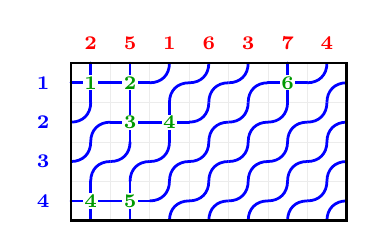
\begin{tikzpicture}[scale=0.5]
  \draw[lightgray, very thin, opacity=0.3] (0,1) grid[step=1] (7,5);
  % Row 1: crossings at 1,2,6
  \draw[blue, line width=1.0pt, line cap=round] (0,4.5) -- (1,4.5);
  \draw[blue, line width=1.0pt, line cap=round] (0.5,4) -- (0.5,5);
  \draw[blue, line width=1.0pt, line cap=round] (1,4.5) -- (2,4.5);
  \draw[blue, line width=1.0pt, line cap=round] (1.5,4) -- (1.5,5);
  \draw[blue, line width=1.0pt] (2,4.5) .. controls (2.3,4.5) and (2.5,4.7) .. (2.5,5);
  \draw[blue, line width=1.0pt] (2.5,4) .. controls (2.5,4.3) and (2.7,4.5) .. (3,4.5);
  \draw[blue, line width=1.0pt] (3,4.5) .. controls (3.3,4.5) and (3.5,4.7) .. (3.5,5);
  \draw[blue, line width=1.0pt] (3.5,4) .. controls (3.5,4.3) and (3.7,4.5) .. (4,4.5);
  \draw[blue, line width=1.0pt] (4,4.5) .. controls (4.3,4.5) and (4.5,4.7) .. (4.5,5);
  \draw[blue, line width=1.0pt] (4.5,4) .. controls (4.5,4.3) and (4.7,4.5) .. (5,4.5);
  \draw[blue, line width=1.0pt, line cap=round] (5,4.5) -- (6,4.5);
  \draw[blue, line width=1.0pt, line cap=round] (5.5,4) -- (5.5,5);
  \draw[blue, line width=1.0pt] (6,4.5) .. controls (6.3,4.5) and (6.5,4.7) .. (6.5,5);
  \draw[blue, line width=1.0pt] (6.5,4) .. controls (6.5,4.3) and (6.7,4.5) .. (7,4.5);
  % Row 2: crossings at 2,3
  \draw[blue, line width=1.0pt] (0,3.5) .. controls (0.3,3.5) and (0.5,3.7) .. (0.5,4);
  \draw[blue, line width=1.0pt] (0.5,3) .. controls (0.5,3.3) and (0.7,3.5) .. (1,3.5);
  \draw[blue, line width=1.0pt, line cap=round] (1,3.5) -- (2,3.5);
  \draw[blue, line width=1.0pt, line cap=round] (1.5,3) -- (1.5,4);
  \draw[blue, line width=1.0pt, line cap=round] (2,3.5) -- (3,3.5);
  \draw[blue, line width=1.0pt, line cap=round] (2.5,3) -- (2.5,4);
  \draw[blue, line width=1.0pt] (3,3.5) .. controls (3.3,3.5) and (3.5,3.7) .. (3.5,4);
  \draw[blue, line width=1.0pt] (3.5,3) .. controls (3.5,3.3) and (3.7,3.5) .. (4,3.5);
  \draw[blue, line width=1.0pt] (4,3.5) .. controls (4.3,3.5) and (4.5,3.7) .. (4.5,4);
  \draw[blue, line width=1.0pt] (4.5,3) .. controls (4.5,3.3) and (4.7,3.5) .. (5,3.5);
  \draw[blue, line width=1.0pt] (5,3.5) .. controls (5.3,3.5) and (5.5,3.7) .. (5.5,4);
  \draw[blue, line width=1.0pt] (5.5,3) .. controls (5.5,3.3) and (5.7,3.5) .. (6,3.5);
  \draw[blue, line width=1.0pt] (6,3.5) .. controls (6.3,3.5) and (6.5,3.7) .. (6.5,4);
  \draw[blue, line width=1.0pt] (6.5,3) .. controls (6.5,3.3) and (6.7,3.5) .. (7,3.5);
  % Row 3: empty
  \draw[blue, line width=1.0pt] (0,2.5) .. controls (0.3,2.5) and (0.5,2.7) .. (0.5,3);
  \draw[blue, line width=1.0pt] (0.5,2) .. controls (0.5,2.3) and (0.7,2.5) .. (1,2.5);
  \draw[blue, line width=1.0pt] (1,2.5) .. controls (1.3,2.5) and (1.5,2.7) .. (1.5,3);
  \draw[blue, line width=1.0pt] (1.5,2) .. controls (1.5,2.3) and (1.7,2.5) .. (2,2.5);
  \draw[blue, line width=1.0pt] (2,2.5) .. controls (2.3,2.5) and (2.5,2.7) .. (2.5,3);
  \draw[blue, line width=1.0pt] (2.5,2) .. controls (2.5,2.3) and (2.7,2.5) .. (3,2.5);
  \draw[blue, line width=1.0pt] (3,2.5) .. controls (3.3,2.5) and (3.5,2.7) .. (3.5,3);
  \draw[blue, line width=1.0pt] (3.5,2) .. controls (3.5,2.3) and (3.7,2.5) .. (4,2.5);
  \draw[blue, line width=1.0pt] (4,2.5) .. controls (4.3,2.5) and (4.5,2.7) .. (4.5,3);
  \draw[blue, line width=1.0pt] (4.5,2) .. controls (4.5,2.3) and (4.7,2.5) .. (5,2.5);
  \draw[blue, line width=1.0pt] (5,2.5) .. controls (5.3,2.5) and (5.5,2.7) .. (5.5,3);
  \draw[blue, line width=1.0pt] (5.5,2) .. controls (5.5,2.3) and (5.7,2.5) .. (6,2.5);
  \draw[blue, line width=1.0pt] (6,2.5) .. controls (6.3,2.5) and (6.5,2.7) .. (6.5,3);
  \draw[blue, line width=1.0pt] (6.5,2) .. controls (6.5,2.3) and (6.7,2.5) .. (7,2.5);
  % Row 4: crossings at 1,2
  \draw[blue, line width=1.0pt, line cap=round] (0,1.5) -- (1,1.5);
  \draw[blue, line width=1.0pt, line cap=round] (0.5,1) -- (0.5,2);
  \draw[blue, line width=1.0pt, line cap=round] (1,1.5) -- (2,1.5);
  \draw[blue, line width=1.0pt, line cap=round] (1.5,1) -- (1.5,2);
  \draw[blue, line width=1.0pt] (2,1.5) .. controls (2.3,1.5) and (2.5,1.7) .. (2.5,2);
  \draw[blue, line width=1.0pt] (2.5,1) .. controls (2.5,1.3) and (2.7,1.5) .. (3,1.5);
  \draw[blue, line width=1.0pt] (3,1.5) .. controls (3.3,1.5) and (3.5,1.7) .. (3.5,2);
  \draw[blue, line width=1.0pt] (3.5,1) .. controls (3.5,1.3) and (3.7,1.5) .. (4,1.5);
  \draw[blue, line width=1.0pt] (4,1.5) .. controls (4.3,1.5) and (4.5,1.7) .. (4.5,2);
  \draw[blue, line width=1.0pt] (4.5,1) .. controls (4.5,1.3) and (4.7,1.5) .. (5,1.5);
  \draw[blue, line width=1.0pt] (5,1.5) .. controls (5.3,1.5) and (5.5,1.7) .. (5.5,2);
  \draw[blue, line width=1.0pt] (5.5,1) .. controls (5.5,1.3) and (5.7,1.5) .. (6,1.5);
  \draw[blue, line width=1.0pt] (6,1.5) .. controls (6.3,1.5) and (6.5,1.7) .. (6.5,2);
  \draw[blue, line width=1.0pt] (6.5,1) .. controls (6.5,1.3) and (6.7,1.5) .. (7,1.5);
  \node[font=\scriptsize\bfseries, text=green!60!black, fill=white, inner sep=0.5pt] at (0.5,4.5) {1};
  \node[font=\scriptsize\bfseries, text=green!60!black, fill=white, inner sep=0.5pt] at (1.5,4.5) {2};
  \node[font=\scriptsize\bfseries, text=green!60!black, fill=white, inner sep=0.5pt] at (5.5,4.5) {6};
  \node[font=\scriptsize\bfseries, text=green!60!black, fill=white, inner sep=0.5pt] at (1.5,3.5) {3};
  \node[font=\scriptsize\bfseries, text=green!60!black, fill=white, inner sep=0.5pt] at (2.5,3.5) {4};
  \node[font=\scriptsize\bfseries, text=green!60!black, fill=white, inner sep=0.5pt] at (0.5,1.5) {4};
  \node[font=\scriptsize\bfseries, text=green!60!black, fill=white, inner sep=0.5pt] at (1.5,1.5) {5};
  \node[font=\scriptsize\bfseries, text=blue, anchor=east] at (-0.3,4.5) {1};
  \node[font=\scriptsize\bfseries, text=blue, anchor=east] at (-0.3,3.5) {2};
  \node[font=\scriptsize\bfseries, text=blue, anchor=east] at (-0.3,2.5) {3};
  \node[font=\scriptsize\bfseries, text=blue, anchor=east] at (-0.3,1.5) {4};
  % Output permutation at top
  \node[font=\scriptsize\bfseries, text=red, anchor=south] at (0.5,5.1) {2};
  \node[font=\scriptsize\bfseries, text=red, anchor=south] at (1.5,5.1) {5};
  \node[font=\scriptsize\bfseries, text=red, anchor=south] at (2.5,5.1) {1};
  \node[font=\scriptsize\bfseries, text=red, anchor=south] at (3.5,5.1) {6};
  \node[font=\scriptsize\bfseries, text=red, anchor=south] at (4.5,5.1) {3};
  \node[font=\scriptsize\bfseries, text=red, anchor=south] at (5.5,5.1) {7};
  \node[font=\scriptsize\bfseries, text=red, anchor=south] at (6.5,5.1) {4};
  \draw[black, line width=1.0pt] (0,1) rectangle (7,5);
\end{tikzpicture}
\caption*{(a) $R$ with $p=3$}
\end{minipage}
\hfill
% Step 2: After deletion
\begin{minipage}{0.22\textwidth}
\centering
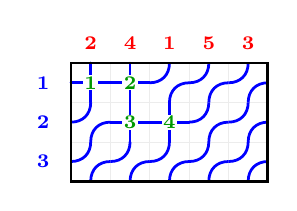
\begin{tikzpicture}[scale=0.5]
  \draw[lightgray, very thin, opacity=0.3] (0,2) grid[step=1] (5,5);
  % Row 1: crossings at 1,2 (no 6)
  \draw[blue, line width=1.0pt, line cap=round] (0,4.5) -- (1,4.5);
  \draw[blue, line width=1.0pt, line cap=round] (0.5,4) -- (0.5,5);
  \draw[blue, line width=1.0pt, line cap=round] (1,4.5) -- (2,4.5);
  \draw[blue, line width=1.0pt, line cap=round] (1.5,4) -- (1.5,5);
  \draw[blue, line width=1.0pt] (2,4.5) .. controls (2.3,4.5) and (2.5,4.7) .. (2.5,5);
  \draw[blue, line width=1.0pt] (2.5,4) .. controls (2.5,4.3) and (2.7,4.5) .. (3,4.5);
  \draw[blue, line width=1.0pt] (3,4.5) .. controls (3.3,4.5) and (3.5,4.7) .. (3.5,5);
  \draw[blue, line width=1.0pt] (3.5,4) .. controls (3.5,4.3) and (3.7,4.5) .. (4,4.5);
  \draw[blue, line width=1.0pt] (4,4.5) .. controls (4.3,4.5) and (4.5,4.7) .. (4.5,5);
  \draw[blue, line width=1.0pt] (4.5,4) .. controls (4.5,4.3) and (4.7,4.5) .. (5,4.5);
  % Row 2: crossings at 2,3
  \draw[blue, line width=1.0pt] (0,3.5) .. controls (0.3,3.5) and (0.5,3.7) .. (0.5,4);
  \draw[blue, line width=1.0pt] (0.5,3) .. controls (0.5,3.3) and (0.7,3.5) .. (1,3.5);
  \draw[blue, line width=1.0pt, line cap=round] (1,3.5) -- (2,3.5);
  \draw[blue, line width=1.0pt, line cap=round] (1.5,3) -- (1.5,4);
  \draw[blue, line width=1.0pt, line cap=round] (2,3.5) -- (3,3.5);
  \draw[blue, line width=1.0pt, line cap=round] (2.5,3) -- (2.5,4);
  \draw[blue, line width=1.0pt] (3,3.5) .. controls (3.3,3.5) and (3.5,3.7) .. (3.5,4);
  \draw[blue, line width=1.0pt] (3.5,3) .. controls (3.5,3.3) and (3.7,3.5) .. (4,3.5);
  \draw[blue, line width=1.0pt] (4,3.5) .. controls (4.3,3.5) and (4.5,3.7) .. (4.5,4);
  \draw[blue, line width=1.0pt] (4.5,3) .. controls (4.5,3.3) and (4.7,3.5) .. (5,3.5);
  % Row 3: empty
  \draw[blue, line width=1.0pt] (0,2.5) .. controls (0.3,2.5) and (0.5,2.7) .. (0.5,3);
  \draw[blue, line width=1.0pt] (0.5,2) .. controls (0.5,2.3) and (0.7,2.5) .. (1,2.5);
  \draw[blue, line width=1.0pt] (1,2.5) .. controls (1.3,2.5) and (1.5,2.7) .. (1.5,3);
  \draw[blue, line width=1.0pt] (1.5,2) .. controls (1.5,2.3) and (1.7,2.5) .. (2,2.5);
  \draw[blue, line width=1.0pt] (2,2.5) .. controls (2.3,2.5) and (2.5,2.7) .. (2.5,3);
  \draw[blue, line width=1.0pt] (2.5,2) .. controls (2.5,2.3) and (2.7,2.5) .. (3,2.5);
  \draw[blue, line width=1.0pt] (3,2.5) .. controls (3.3,2.5) and (3.5,2.7) .. (3.5,3);
  \draw[blue, line width=1.0pt] (3.5,2) .. controls (3.5,2.3) and (3.7,2.5) .. (4,2.5);
  \draw[blue, line width=1.0pt] (4,2.5) .. controls (4.3,2.5) and (4.5,2.7) .. (4.5,3);
  \draw[blue, line width=1.0pt] (4.5,2) .. controls (4.5,2.3) and (4.7,2.5) .. (5,2.5);
  \node[font=\scriptsize\bfseries, text=green!60!black, fill=white, inner sep=0.5pt] at (0.5,4.5) {1};
  \node[font=\scriptsize\bfseries, text=green!60!black, fill=white, inner sep=0.5pt] at (1.5,4.5) {2};
  \node[font=\scriptsize\bfseries, text=green!60!black, fill=white, inner sep=0.5pt] at (1.5,3.5) {3};
  \node[font=\scriptsize\bfseries, text=green!60!black, fill=white, inner sep=0.5pt] at (2.5,3.5) {4};
  \node[font=\scriptsize\bfseries, text=blue, anchor=east] at (-0.3,4.5) {1};
  \node[font=\scriptsize\bfseries, text=blue, anchor=east] at (-0.3,3.5) {2};
  \node[font=\scriptsize\bfseries, text=blue, anchor=east] at (-0.3,2.5) {3};
  % Output permutation at top
  \node[font=\scriptsize\bfseries, text=red, anchor=south] at (0.5,5.1) {2};
  \node[font=\scriptsize\bfseries, text=red, anchor=south] at (1.5,5.1) {4};
  \node[font=\scriptsize\bfseries, text=red, anchor=south] at (2.5,5.1) {1};
  \node[font=\scriptsize\bfseries, text=red, anchor=south] at (3.5,5.1) {5};
  \node[font=\scriptsize\bfseries, text=red, anchor=south] at (4.5,5.1) {3};
  \draw[black, line width=1.0pt] (0,2) rectangle (5,5);
\end{tikzpicture}
\caption*{(b) After delete (1,6)}
\end{minipage}
\hfill
% Step 3: Zero out row 3
\begin{minipage}{0.22\textwidth}
\centering
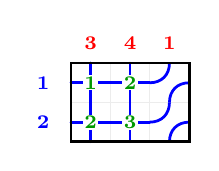
\begin{tikzpicture}[scale=0.5]
  \draw[lightgray, very thin, opacity=0.3] (0,3) grid[step=1] (3,5);
  % Row 1: crossings at 1,2
  \draw[blue, line width=1.0pt, line cap=round] (0,4.5) -- (1,4.5);
  \draw[blue, line width=1.0pt, line cap=round] (0.5,4) -- (0.5,5);
  \draw[blue, line width=1.0pt, line cap=round] (1,4.5) -- (2,4.5);
  \draw[blue, line width=1.0pt, line cap=round] (1.5,4) -- (1.5,5);
  \draw[blue, line width=1.0pt] (2,4.5) .. controls (2.3,4.5) and (2.5,4.7) .. (2.5,5);
  \draw[blue, line width=1.0pt] (2.5,4) .. controls (2.5,4.3) and (2.7,4.5) .. (3,4.5);
  % Row 2: crossings at 1,2
  \draw[blue, line width=1.0pt, line cap=round] (0,3.5) -- (1,3.5);
  \draw[blue, line width=1.0pt, line cap=round] (0.5,3) -- (0.5,4);
  \draw[blue, line width=1.0pt, line cap=round] (1,3.5) -- (2,3.5);
  \draw[blue, line width=1.0pt, line cap=round] (1.5,3) -- (1.5,4);
  \draw[blue, line width=1.0pt] (2,3.5) .. controls (2.3,3.5) and (2.5,3.7) .. (2.5,4);
  \draw[blue, line width=1.0pt] (2.5,3) .. controls (2.5,3.3) and (2.7,3.5) .. (3,3.5);
  \node[font=\scriptsize\bfseries, text=green!60!black, fill=white, inner sep=0.5pt] at (0.5,4.5) {1};
  \node[font=\scriptsize\bfseries, text=green!60!black, fill=white, inner sep=0.5pt] at (1.5,4.5) {2};
  \node[font=\scriptsize\bfseries, text=green!60!black, fill=white, inner sep=0.5pt] at (0.5,3.5) {2};
  \node[font=\scriptsize\bfseries, text=green!60!black, fill=white, inner sep=0.5pt] at (1.5,3.5) {3};
  \node[font=\scriptsize\bfseries, text=blue, anchor=east] at (-0.3,4.5) {1};
  \node[font=\scriptsize\bfseries, text=blue, anchor=east] at (-0.3,3.5) {2};
  % Output permutation at top
  \node[font=\scriptsize\bfseries, text=red, anchor=south] at (0.5,5.1) {3};
  \node[font=\scriptsize\bfseries, text=red, anchor=south] at (1.5,5.1) {4};
  \node[font=\scriptsize\bfseries, text=red, anchor=south] at (2.5,5.1) {1};
  \draw[black, line width=1.0pt] (0,3) rectangle (3,5);
\end{tikzpicture}
\caption*{(c) $\zeromap(R_k)$}
\end{minipage}
\hfill
% Step 4: Insert back
\begin{minipage}{0.22\textwidth}
\centering
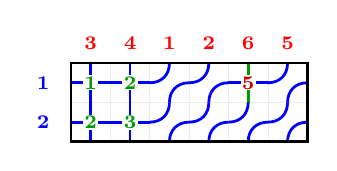
\begin{tikzpicture}[scale=0.5]
  \draw[lightgray, very thin, opacity=0.3] (0,3) grid[step=1] (6,5);
  % Row 1: crossings at 1,2,5
  \draw[blue, line width=1.0pt, line cap=round] (0,4.5) -- (1,4.5);
  \draw[blue, line width=1.0pt, line cap=round] (0.5,4) -- (0.5,5);
  \draw[blue, line width=1.0pt, line cap=round] (1,4.5) -- (2,4.5);
  \draw[blue, line width=1.0pt, line cap=round] (1.5,4) -- (1.5,5);
  \draw[blue, line width=1.0pt] (2,4.5) .. controls (2.3,4.5) and (2.5,4.7) .. (2.5,5);
  \draw[blue, line width=1.0pt] (2.5,4) .. controls (2.5,4.3) and (2.7,4.5) .. (3,4.5);
  \draw[blue, line width=1.0pt] (3,4.5) .. controls (3.3,4.5) and (3.5,4.7) .. (3.5,5);
  \draw[blue, line width=1.0pt] (3.5,4) .. controls (3.5,4.3) and (3.7,4.5) .. (4,4.5);
  \draw[blue, line width=1.0pt, line cap=round] (4,4.5) -- (5,4.5);
  \draw[green!60!black, line width=1.0pt, line cap=round] (4.5,4) -- (4.5,5);
  \draw[blue, line width=1.0pt] (5,4.5) .. controls (5.3,4.5) and (5.5,4.7) .. (5.5,5);
  \draw[blue, line width=1.0pt] (5.5,4) .. controls (5.5,4.3) and (5.7,4.5) .. (6,4.5);
  % Row 2: crossings at 1,2
  \draw[blue, line width=1.0pt, line cap=round] (0,3.5) -- (1,3.5);
  \draw[blue, line width=1.0pt, line cap=round] (0.5,3) -- (0.5,4);
  \draw[blue, line width=1.0pt, line cap=round] (1,3.5) -- (2,3.5);
  \draw[blue, line width=1.0pt, line cap=round] (1.5,3) -- (1.5,4);
  \draw[blue, line width=1.0pt] (2,3.5) .. controls (2.3,3.5) and (2.5,3.7) .. (2.5,4);
  \draw[blue, line width=1.0pt] (2.5,3) .. controls (2.5,3.3) and (2.7,3.5) .. (3,3.5);
  \draw[blue, line width=1.0pt] (3,3.5) .. controls (3.3,3.5) and (3.5,3.7) .. (3.5,4);
  \draw[blue, line width=1.0pt] (3.5,3) .. controls (3.5,3.3) and (3.7,3.5) .. (4,3.5);
  \draw[blue, line width=1.0pt] (4,3.5) .. controls (4.3,3.5) and (4.5,3.7) .. (4.5,4);
  \draw[blue, line width=1.0pt] (4.5,3) .. controls (4.5,3.3) and (4.7,3.5) .. (5,3.5);
  \draw[blue, line width=1.0pt] (5,3.5) .. controls (5.3,3.5) and (5.5,3.7) .. (5.5,4);
  \draw[blue, line width=1.0pt] (5.5,3) .. controls (5.5,3.3) and (5.7,3.5) .. (6,3.5);
  \node[font=\scriptsize\bfseries, text=green!60!black, fill=white, inner sep=0.5pt] at (0.5,4.5) {1};
  \node[font=\scriptsize\bfseries, text=green!60!black, fill=white, inner sep=0.5pt] at (1.5,4.5) {2};
  \node[font=\scriptsize\bfseries, text=red!80!black, fill=white, inner sep=0.5pt] at (4.5,4.5) {5};
  \node[font=\scriptsize\bfseries, text=green!60!black, fill=white, inner sep=0.5pt] at (0.5,3.5) {2};
  \node[font=\scriptsize\bfseries, text=green!60!black, fill=white, inner sep=0.5pt] at (1.5,3.5) {3};
  \node[font=\scriptsize\bfseries, text=blue, anchor=east] at (-0.3,4.5) {1};
  \node[font=\scriptsize\bfseries, text=blue, anchor=east] at (-0.3,3.5) {2};
  % Output permutation at top
  \node[font=\scriptsize\bfseries, text=red, anchor=south] at (0.5,5.1) {3};
  \node[font=\scriptsize\bfseries, text=red, anchor=south] at (1.5,5.1) {4};
  \node[font=\scriptsize\bfseries, text=red, anchor=south] at (2.5,5.1) {1};
  \node[font=\scriptsize\bfseries, text=red, anchor=south] at (3.5,5.1) {2};
  \node[font=\scriptsize\bfseries, text=red, anchor=south] at (4.5,5.1) {6};
  \node[font=\scriptsize\bfseries, text=red, anchor=south] at (5.5,5.1) {5};
  \draw[black, line width=1.0pt] (0,3) rectangle (6,5);
\end{tikzpicture}
\caption*{(d) After $\ins{5}{1}$}
\end{minipage}

\vspace{0.3cm}

% Step 5: Final with R>p
\begin{minipage}{0.45\textwidth}
\centering
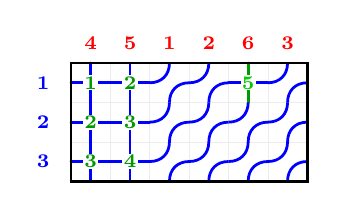
\begin{tikzpicture}[scale=0.5]
  \draw[lightgray, very thin, opacity=0.3] (0,1) grid[step=1] (6,4);
  % Row 1: crossings at 1,2,5
  \draw[blue, line width=1.0pt, line cap=round] (0,3.5) -- (1,3.5);
  \draw[blue, line width=1.0pt, line cap=round] (0.5,3) -- (0.5,4);
  \draw[blue, line width=1.0pt, line cap=round] (1,3.5) -- (2,3.5);
  \draw[blue, line width=1.0pt, line cap=round] (1.5,3) -- (1.5,4);
  \draw[blue, line width=1.0pt] (2,3.5) .. controls (2.3,3.5) and (2.5,3.7) .. (2.5,4);
  \draw[blue, line width=1.0pt] (2.5,3) .. controls (2.5,3.3) and (2.7,3.5) .. (3,3.5);
  \draw[blue, line width=1.0pt] (3,3.5) .. controls (3.3,3.5) and (3.5,3.7) .. (3.5,4);
  \draw[blue, line width=1.0pt] (3.5,3) .. controls (3.5,3.3) and (3.7,3.5) .. (4,3.5);
  \draw[blue, line width=1.0pt, line cap=round] (4,3.5) -- (5,3.5);
  \draw[green!60!black, line width=1.0pt, line cap=round] (4.5,3) -- (4.5,4);
  \draw[blue, line width=1.0pt] (5,3.5) .. controls (5.3,3.5) and (5.5,3.7) .. (5.5,4);
  \draw[blue, line width=1.0pt] (5.5,3) .. controls (5.5,3.3) and (5.7,3.5) .. (6,3.5);
  % Row 2: crossings at 1,2
  \draw[blue, line width=1.0pt, line cap=round] (0,2.5) -- (1,2.5);
  \draw[blue, line width=1.0pt, line cap=round] (0.5,2) -- (0.5,3);
  \draw[blue, line width=1.0pt, line cap=round] (1,2.5) -- (2,2.5);
  \draw[blue, line width=1.0pt, line cap=round] (1.5,2) -- (1.5,3);
  \draw[blue, line width=1.0pt] (2,2.5) .. controls (2.3,2.5) and (2.5,2.7) .. (2.5,3);
  \draw[blue, line width=1.0pt] (2.5,2) .. controls (2.5,2.3) and (2.7,2.5) .. (3,2.5);
  \draw[blue, line width=1.0pt] (3,2.5) .. controls (3.3,2.5) and (3.5,2.7) .. (3.5,3);
  \draw[blue, line width=1.0pt] (3.5,2) .. controls (3.5,2.3) and (3.7,2.5) .. (4,2.5);
  \draw[blue, line width=1.0pt] (4,2.5) .. controls (4.3,2.5) and (4.5,2.7) .. (4.5,3);
  \draw[blue, line width=1.0pt] (4.5,2) .. controls (4.5,2.3) and (4.7,2.5) .. (5,2.5);
  \draw[blue, line width=1.0pt] (5,2.5) .. controls (5.3,2.5) and (5.5,2.7) .. (5.5,3);
  \draw[blue, line width=1.0pt] (5.5,2) .. controls (5.5,2.3) and (5.7,2.5) .. (6,2.5);
  % Row 3: crossings at 1,2 (from R>p shifted)
  \draw[blue, line width=1.0pt, line cap=round] (0,1.5) -- (1,1.5);
  \draw[blue, line width=1.0pt, line cap=round] (0.5,1) -- (0.5,2);
  \draw[blue, line width=1.0pt, line cap=round] (1,1.5) -- (2,1.5);
  \draw[blue, line width=1.0pt, line cap=round] (1.5,1) -- (1.5,2);
  \draw[blue, line width=1.0pt] (2,1.5) .. controls (2.3,1.5) and (2.5,1.7) .. (2.5,2);
  \draw[blue, line width=1.0pt] (2.5,1) .. controls (2.5,1.3) and (2.7,1.5) .. (3,1.5);
  \draw[blue, line width=1.0pt] (3,1.5) .. controls (3.3,1.5) and (3.5,1.7) .. (3.5,2);
  \draw[blue, line width=1.0pt] (3.5,1) .. controls (3.5,1.3) and (3.7,1.5) .. (4,1.5);
  \draw[blue, line width=1.0pt] (4,1.5) .. controls (4.3,1.5) and (4.5,1.7) .. (4.5,2);
  \draw[blue, line width=1.0pt] (4.5,1) .. controls (4.5,1.3) and (4.7,1.5) .. (5,1.5);
  \draw[blue, line width=1.0pt] (5,1.5) .. controls (5.3,1.5) and (5.5,1.7) .. (5.5,2);
  \draw[blue, line width=1.0pt] (5.5,1) .. controls (5.5,1.3) and (5.7,1.5) .. (6,1.5);
  \node[font=\scriptsize\bfseries, text=green!60!black, fill=white, inner sep=0.5pt] at (0.5,3.5) {1};
  \node[font=\scriptsize\bfseries, text=green!60!black, fill=white, inner sep=0.5pt] at (1.5,3.5) {2};
  \node[font=\scriptsize\bfseries, text=green!80!black, fill=white, inner sep=0.5pt] at (4.5,3.5) {5};
  \node[font=\scriptsize\bfseries, text=green!60!black, fill=white, inner sep=0.5pt] at (0.5,2.5) {2};
  \node[font=\scriptsize\bfseries, text=green!60!black, fill=white, inner sep=0.5pt] at (1.5,2.5) {3};
  \node[font=\scriptsize\bfseries, text=green!60!black, fill=white, inner sep=0.5pt] at (0.5,1.5) {3};
  \node[font=\scriptsize\bfseries, text=green!60!black, fill=white, inner sep=0.5pt] at (1.5,1.5) {4};
  \node[font=\scriptsize\bfseries, text=blue, anchor=east] at (-0.3,3.5) {1};
  \node[font=\scriptsize\bfseries, text=blue, anchor=east] at (-0.3,2.5) {2};
  \node[font=\scriptsize\bfseries, text=blue, anchor=east] at (-0.3,1.5) {3};
  % Output permutation at top
  \node[font=\scriptsize\bfseries, text=red, anchor=south] at (0.5,4.1) {4};
  \node[font=\scriptsize\bfseries, text=red, anchor=south] at (1.5,4.1) {5};
  \node[font=\scriptsize\bfseries, text=red, anchor=south] at (2.5,4.1) {1};
  \node[font=\scriptsize\bfseries, text=red, anchor=south] at (3.5,4.1) {2};
  \node[font=\scriptsize\bfseries, text=red, anchor=south] at (4.5,4.1) {6};
  \node[font=\scriptsize\bfseries, text=red, anchor=south] at (5.5,4.1) {3};
  \draw[black, line width=1.0pt] (0,1) rectangle (6,4);
\end{tikzpicture}
\caption*{(e) Final $\zeromap^{(p)}(R)$ with $R_{>p}$ reattached}
\end{minipage}

\caption{Example of $\zeromap^{(p)}$ operation with $p=3$. Starting with (a) $R$ where row 3 is empty, we identify element $(1,6)$ creates maxd $> p$. (b) After deleting it (storing row 1 in $A_1$). (c) Apply $\zeromap$ to get 2-row graph. (d) Insert back at row 1 with $k=d_1-1=5$ (shown in red). (e) Reattach $R_{>p}$ shifted down to get final result.}
\label{figure:zpexample}
\end{figure}

\begin{definition}
Let $R$ be an RC graph. We define an RC graph $\overline{R}$ and a sequence $\mathtt{strip}(R)$ as follows. Let $\maxd(R)=n$, set $R_0=R$, and set $A_0=()$. While $\maxd(R_i)> n -1$, delete the element $(a,b)\in R_i$ such that $\rtt_{R_i}(a,b)=(\maxd(R_i), \maxd(R_i) + 1)$ to obtain $R_{i+1}$, and add $a$ to $A_i$ to obtain $A_{i+1}$. When the algorithm terminates at step $k$, set
$$\mathtt{strip}(R) = A_k$$
and set $\overline{R} = R_k$.
\end{definition}

\begin{lemma} \label{lemma:reconstruct}
Let $R$ be an RC graph. Then
$$R = \ins{\maxd(R)}{\mathtt{strip}(R)} \overline{R}$$
\end{lemma}
\begin{proof}
Let $n=\maxd(R)$. We prove this by induction on $\code_n(R)$. Let $(i,j)$ be the location of the descent $n$ in $R$. If $\code_n(R)=1$, then we know that insertion of $i$ into $\overline{R}$ returns an RC graph with the same weight and permutation as $R$, the latter assertion because the only $n$-reflection that increases the length of $\wof{\overline{R}}$ by exactly $1$ is $s_n$. By the exchange property, there is precisely one location in row $i$ that this $n$-reflection can be inserted, and we have the result when $\code_{n}(R)=1$.

Assume the inductive hypothesis that we have the result for $\code_n(R) = k$ for some $k\geq 1$ and additionally that insertion order of reflections has been $(n, n+1),\ldots,(n,n+k)$. Assume $\mathtt{strip}(R) = (r_1,\ldots,r_{k+1})$ in increasing order and we have inserted all of $r_2,\ldots,r_{k+1}$ in Algorithm \ref{algorithm:insertion}. By the induction hypothesis, the RC graph $R'$ we have at this point has permutation $\code_i{R'} = \code_i{R}$ for $i<n$ and $\code_n(R') = k$, and we have equality of $R'$ with $R$ except deletion of the root $(n, n+k + 1)$. Since $\wof{R'}(n) < \wof{R'}(n+k+1)$, the only $n$-reflection that can be inserted to increase the length of $\wof{R'}$ by $1$ is $(n, n+k+1)$. By pipe considerations, this must be inserted in column $c = n + k + 1 - r_1$. Since this is the only possible insertion location and the permutation is the same as $\wof{R}$, we have the result by induction.
\end{proof}

\begin{theorem}
The RC graphs for a permutation $w$ are in bijection with the set of tuples of weakly decreasing sequences $(A_1,\ldots,A_k)$ such that $|A_i| = \code_i(w)$ for all $i$ and (labeled bruhat paths insertion)
LABELED BRUHAT PATHS

FIDDLE WITH THE BEEPS ONE ROW EMPTY GOOD STUFF
\end{theorem}

\begin{theorem}
Let $R\in\BRC(w,n)^{(0,p)}$ be the set of all bounded RC graphs with $\hr(R)=n$ such that row $p$ of $R$ is empty. Then we have that the restriction of $\zeromap^{(p)}$ is a bijection
$$\zeromap^{(p)}:\BRC(w,n)^{(0,p)}=\bigcup_{\substack{w\downvar{p} w'\\\ell(w)=\ell(w')}} \BRC(w', n-1)$$
satisfying $\wtt(\zeromap^{(p)}(R)) = (i_1,\ldots,i_{p-1},i_{p+1},\ldots,i_{n})$, where $\wtt(R)=(i_1,\ldots,i_n)$.
\end{theorem}
\begin{proof}
Consider first the special case that $R_{>p}$ is empty. Let $w_0 = \wof{\zeromap(R_k)}$. Then we know that
$$R_k\downvar{p} \zeromap(R_k)$$
Since every element of $A_k$ is less than $p$ and $d_k>p$, the insertion $\ins{d_k-1}{A_k}\zeromap(R_k)$ only adds right roots $(a,b)$ with $a<p$ and $b>p$. Thus
$$\ins{d_k}{A_k}R_k\downvar{p} \ins{d_k-1}{A_k}\zeromap(R_k)$$
We assert the (descending) inductive hypothesis that for some index $j$ we have
$$\ins{d_j}{A_j}\cdots\ins{d_k}{A_k}R_k\downvar{p} \ins{d_j-1}{A_j}\cdots\ins{d_k-1}{A_k}\zeromap(R_k)$$
Then the induction step follows with precisely the same reasoning; since every element of $A_{j-1}$ is less than $p$ and $d_{j-1}>p$, the insertion $\ins{d_{j-1}-1}{A_{j-1}}$ only adds right roots $(a,b)$ with $a<p$ and $b>p$. Thus
$$\ins{d_{j-1}}{A_{j-1}}\cdots\ins{d_k}{A_k}R_k\downvar{p} \ins{d_{j-1}-1}{A_{j-1}}\cdots\ins{d_k-1}{A_k}\zeromap(R_k)$$
and the result follows by induction in the special case that $R_{>p}$ is empty, where we invoke Lemma \ref{lemma:reconstruct} to assert that the left-hand side is equal to $R$.

Since the row was initially empty, we have at our disposal the exchange property on $R_{>p}$, shifting the reflections down a row to obtain the general case.
\end{proof}

Braid relation invariance

\subsection{Preservation of the Demazure crystal structure}

RC-graphs have a Demazure crystal structure defined by Assaf and Schilling in \cite{assaf2018demazure}. Namely, they define operators $e_i:\RC(w)\to\RC(w)\cup\{\emptyset\}$ and $f_i:\RC(w)\to\RC(w)\cup\{\emptyset\}$ for each $i\geq 1$ as follows. 

\begin{definition}
Consider elements $(i, j)\in R$ and $(i+1, k)\in R$. The pairing algorithm starts with the largest $j$ in row $i$ and pairs $(i, j)$ with $(i+1, k)$ where $k$ is the smallest such that $k \geq j$. If no such $k$ exists, then $(i, j)$ is unpaired. The algorithm continues by considering the next largest $j$ in row $i$ and repeating the process until all elements in row $i$ have been considered.

Define $R_i$ to be the set of unpaired elements in row $i$ after applying the pairing algorithm between rows $i$ and $i+1$, and define $L_i$ to be the set of unpaired elements in row $i+1$. Then $f_i(R)$ is defined by removing the leftmost element $(i, j)$ from $R_i$ and adding the element $(i + 1, k)$ to $R$, where $k$ is the largest value such that $(i+1,k)\notin R$ and $k < j$. If $R_i$ is empty or $k$ does not exist, then $f_i(R) = \emptyset$. Similarly, $e_i(R)$ is defined by removing the rightmost element $(i + 1, k)$ from $L_i$ and adding the element $(i, j)$ to $R$, where $j$ is the smallest value such that $(i,j)\notin R$ and $j > k$. If $L_i$ is empty, then $e_i(R) = \emptyset$.
\end{definition}

We may transport this structure to bounded RC graphs as  operators $e_i:\mathcal{RC}(w,n)\to\mathcal{RC}(w,n)\cup\{\emptyset\}$ and $f_i:\mathcal{RC}(w,n)\to\mathcal{RC}(w,n)\cup\{\emptyset\}$ by preserving the bound:
$$e_i(R) = e_i(R)$$
$$f_i(R)=f_i(R)$$

where the bound is preserved (i.e., $\hr(f_i(R)) = \hr(R)$ when $f_i(R)\neq\emptyset$).



\newcommand{\ckeq}{\sim}
\newcommand{\ege}{\widetilde{\mathrm{eg}}}
\begin{definition}
An RC graph $R$ has a uniquely associated reduced word $\mathrm{word}(R)=(s_{i_1},\ldots,s_{i_N})$. Recall the Coxeter-Knuth relation $\ege$ defined by
$$j\ i\ k \ckeq j\ k\ i$$
and
$$k\ i\ j \ckeq i\ k\ j$$
if $i<j<k$, and
$$i\ i+1\ i \ckeq i+1\ i\ i+1$$
For an RC graph $R$, define $N(R)$ to be the maximum letter in $R$. Then define
$$\ege(R) = (N(R) + 1 - i_1, \ldots, N(R) + 1 - i_N)$$
Via the Edelman-Greene insertion algorithm, we may define a pair
$$(P, Q)$$
of tableaux of the same shape such that the reading word of $P$ is CK-equivalent to $\ege(R)$ and $Q$, the recording tableau, is standard. Define $\mathtt{tab}(R)$ to be the tableau of the same shape as $Q$ such that the entry in box $(i, j)$ is the row index of the box in $R$ that was inserted to create box $(i, j)$ in $P$.
\end{definition}

\begin{lemma}
	We have that $\mathtt{tab}(R)$ is a semistandard Young tableau of shape $\mathrm{shape}(Q)$, and the map
	$$R\mapsto \mathtt{tab}(R)$$
	 is a morphism of crystal graphs into $B(\mathrm{shape}(Q))$. 
\end{lemma}
\begin{proof}
Suppose $R$ is a highest weight. Then $\wtt(R)$ is a partition. By the highest weight condition, the longest increasing subsequence of $\ege(R)$ is of length $\wtt(R)_1$ and is precisely the first row read in the grid order. By the Edelman-Greene correspondence \cite{edelman1987balanced}, the first row of $P$ has length equal to the length of the longest increasing subsequence of $\ege(R)$. Hence, the first row of $P$ has length $\wtt(R)_1$. By similar reasoning on the subsequent rows, we have that $\mathrm{shape}(P) = \wtt(R)$. We then have that $\mathtt{tab}(R)$ is the unique Yamanouchi tableau of shape $\wtt(R)$, establishing the claim for highest weights. The general case follows from the rigidity of the Demazure crystal structure \cite{assaf2018demazure}; since the function is weight-preserving, it is a morphism of crystal graphs.
\end{proof}

\begin{theorem}
	% Let $R,R'$ be RC graphs. Then $\mathrm{hw}(R) = \mathrm{hw}(R')$ if and only if $\ege(R) \ckeq \ege(R')$.
  The distinct Demazure crystals that make up $\RC(w)$ are in bijection with the Coxeter-Knuth equivalence classes of reduced words for $w_0ww_0$ via the map $R\mapsto \ege(R)$, with $R\mapsto \mathtt{tab}(R)$ being a homomorphism of crystal graphs into $B(\lambda)$, where $\lambda=\mathrm{shape}(P(\ege(R)))$.
\end{theorem}
\begin{proof}
By \cite[Theorem~4.11]{morse2016crystal}, if $e_i(R)\neq \emptyset$, then $R$ and $e_i(R)$ have the same Edelman-Greene insertion tableau. Since conjugation by $w_0$ is an automorphism of Coxeter-Knuth equivalence, so do $\ege(R)$ and $\ege(e_i(R))$. The shape is determined inductively. Suppose $R$ is a highest weight element and consider $\mathtt{word}(R)$. The first row of $R$ forms a word that corresponds to an initial increasing subsequence of $\ege(R)$. If there were a letter in some row below the first that is smaller than the last letter of the first row, then some raising operator would yield a nonempty result, contradicting the fact that $R$ is a highest weight. Thus, the first row of $P(\ege(R))$ has length equal to the length of the first row of $R$. The rest follows by induction on the remaining rows.
\end{proof}

\begin{definition}
Let $\RC(w, n)^0$ be the set of bounded RC graphs $R$ with $\hr(R)=n$ such that $\wof{R} = w$ and row $n$ is empty. We define a function $\zeromap_*^R:R\to R'$, where $\zeromap(R) = (R',n-1)$ and $w'=\wof{R'}$, as follows. Clearly if $\code_n(w) = 0$, then $\zeromap_*^R$ is the identity map. 

Consider now the case where $\code_n(w) = 1$. The initial deletion of $(i,j)$ with $\rtt_R(i,j) = (n, n+1)$ results in an RC graph $R_0 = R\setminus\{(i,j)\}$ with $\wof{R_1} = w s_n$, after which we add $(n,1)$ to obtain $R_1$. Let
$$f_1:R_1\to R$$
be the identity. Afterwards, $(i_1, j_1)$ is inserted into $R_1$ to obtain $R_2$. Set
$$f_1(i_1,j_1) = (i,j)$$
and
$$f_1(a,b) = (a,b)$$
otherwise.

At this point, rectification may be required. In that case, we delete some element $(i_1', j_1')$ from $R_2$ such that $i_1'<i_1$ and $\rtt_{R_2}(i_1', j_1') = \rtt_{R_2}(i_1, j_1)$. Afterwards, we add $(i_1', j_2)$ to obtain $R_2'$. Set
$$f_2(i_1', j_2) = (i_1', j_1')$$
and
$$f_2(a,b) = f_1(a,b)$$
otherwise. Continuing in this manner, we eventually obtain $R'$. Pieicing all of the maps defined at each step gives the desired map. The same method works for $\code_n(w) > 1$ by induction.
\end{definition}

\begin{lemma} \label{lemma:crystalpair}
Let $(R, n)\in \RC(w, n)^0$ and suppose $\zeromap(R) = (R', n-1)$. Then for any $(a,b)\in R'$, $(a,b)$ is paired in the $i,i+1$ pairing in $R'$ if any only if $\zeromap_*^R(a,b)$ is paired in the $i,i+1$ pairing in $R$.
\end{lemma}
\begin{proof}
  This is true for $a=i$ because at most one root is changed in row $i$ and it has moved to the left. For $a=i+1$, the only way that the pairing status could change is if a root in row $i$ moved past an unpaired root in row $i+1$. However, by construction of the insertion algorithm, this cannot happen since a root that was already inserted into row $i+1$ was deleted from row $i$ in the rectification process, and the new inserted root occurs to the left.
\end{proof}

\begin{theorem} \label{theorem:zcrystal}
	Let $w\in S_\infty$ and $n>0$ be such that $\maxd(w)\leq n$. Then 
	$$\zeromap:\RC(w, n)^0\to \bigcup_{w\downvar{n} w'}\RC(w', n-1)$$ 
	is a weight-preserving isomorphism of crystal graphs.
\end{theorem}
\begin{proof}
The existence of the map $\zeromap_*^R$ and the previous lemma establish that $\zeromap$ is a bijection (by Theorem \ref{theorem:zero_bijection}) that preserves both weights and the lengths of $i$-strings. Hence it is a weight-preserving isomorphism of crystal graphs.
\end{proof}


\subsection{Crystal divided differences}

Let $R$ be an RC graph and let $i>0$ be an integer. We define $\rcdd^iR$, an element of $\RC$, as follows. Define
$$\rcdd^iR=0$$
unless $s_i$ is a right descent of $\wof{R}$ and there exists $(i,j)\in R$ such that $\rtt_R(i, j) = (i, i+1)$. If these latter two conditions are satisfied, define 
$$R'=R\setminus \{(i, j)\}$$
where $\rtt_R(i,j) = (i, i+1)$. If $e_i(R')\neq \emptyset$, define $\rcdd^iR=0$. Otherwise, define
$$\rcdd^iR = \sum_{p=0}^{\varphi_i(R')}f_i^pR'$$
\begin{lemma} \label{lemma:divdiffunique}
	Let $R$ be an RC graph and let $i>0$ be an integer. If $s_i$ is not a right descent of $\wof{R}$, then there is a unique $R'$ such that the coefficient of $R$ in $\rcdd^iR'$ is $1$, and for other $R'$ the coefficient is $0$.
\end{lemma}
\begin{proof}
	Suppose $s_i$ is not a right descent of $\wof{R}$. Assume without loss of generality that $e_iR = \emptyset$. If $(i+1, 1)\notin R$, then $(i,1)\notin R$ because $s_i$ is not a right descent of $\wof{R}$. In that case, let $R' = R\cup\{(i,1)\}$. Then 
	$$\rcdd^iR' = R + \text{other terms}$$ 
	If instead $(i+1, 1)\in R$, since $e_i(R)=\emptyset$ it follows that $(i, 1)\in R$, and if $j$ is the maximum value such that $(i+1,j')\in R$ for all $j'<j$, it follows that $(i,j')\in R$ for all $j'<j$. We must have that $(i,j+1)\notin R$, because $\rtt_R(i, j+1)=(i, i+1)$. Setting $R'=R\cup \{(i, j+1)\}$ gives us the result.
\end{proof}

\begin{theorem} \label{theorem:divdiffschubert}
	Suppose $w\in S_\infty$ and $i >0$. If $i$ is not a right descent of $w$, then
	$$\rcdd^i\mathcal{S}_w(n) = 0$$
	Otherwise,
	$$\rcdd^i\mathcal{S}_w(n) = \mathcal{S}_{ws_i}(n)$$
\end{theorem}
\begin{proof}
	The result is trivial if $i$ is not a right descent of $w$. Suppose $i$ is a right descent of $w$. By Lemma \ref{lemma:divdiffunique}, for each RC graph $R$ such that $\wof{R} = ws_i$, there is a unique RC graph $R'$ such that the coefficient of $R$ in $\rcdd^iR'$ is $1$. Since $\wof{R'} = w$, the result follows.
\end{proof}

\begin{corollary} \label{corollary:generateschubert}
Suppose $R$ is an RC graph such that $\wof{R} = w$ is dominant. Then for any reduced word $(s_{i_1}, s_{i_2}, \ldots, s_{i_m})$ for a permutation $u$ such that
$$\ell(wu^{-1}) = \ell(w) - \ell(u)$$
we have that
$$\rcdd^{i_1}\rcdd^{i_2}\cdots \rcdd^{i_m}R = \mathcal{S}_{wu^{-1}}(n)$$
for sufficiently large $n$.
\end{corollary}


\begin{definition}
For a permutation $w$, define the \emph{principal RC graph} $R^0(w)$ of $w$ to be
$$R^0(w) = \{(i,j)\mid 1\leq j\leq \code_i(w)\}$$

We say that row $i$ of an RC graph $R$ has a \emph{ledge} at column $j$ if the configuration of boxes in rows $i$ and $i+1$ satisfy $(i,j)\in R$, $(i+1,j)\notin  R$, $\rtt_R(i,j)=(i,i+1)$, and for all $j' < j$ we have that $(i,j')\in R$ and $(i+1,j')\in R$, as shown in in Figure \ref{figure:ledge}.
\end{definition}

\begin{proposition} \label{proposition:divdiffprincipal}
Let $R$ be an RC graph and let $w=\wof{R}$. Then the following are equivalent.
\begin{enumerate}
\item for any reduced word $(s_{i_1}, s_{i_2}, \ldots, s_{i_m})$ for $w$, we have
$$\rcdd^{i_1}\rcdd^{i_2}\cdots \rcdd^{i_m}R \neq 0$$

\item $R = R^0(w)$.
\end{enumerate}
\end{proposition}
\begin{proof}
For (1)$\Rightarrow$(2), we proceed by induction on length. For (1) to be true, in particular if $n=\maxd(\wof{R})$ we have that $(n,1)\in R$. Applying $\rcdd^n$ and lowering operators (necessarily maximally) results in a term being an RC graph which has the same recursive property, which by the inductive hypothesis is $R^0(ws_n)$, which implies that row $n$ of $R$ has length $\code_n(w)$. Choosing our reduced word carefully, we obtain in the process as some nonzero term an RC graph for $w'$ with $\code_k(w') = \code_k(w)$ for all $k<n$ and $\code_n(w')=0$ that has the same property, and hence is prinicipal by the induction hypothesis. It follows that $R$ is principal as well.

For (2)$\Rightarrow$(1), we again proceed by induction on length. If $w$ has no descents, the statement is vacuous. For a principal RC graph $R^0(w)$ for some $w$ with $\ell(w)>0$ and we have the result for smaller lengths, suppose $i$ is a descent of $w$. Then $\code_i(w) > \code_{i+1}(w)$. In particular, if we let $j = \code_{i+1}(w) + 1$, then $(i,j)$ is a ledge of $R^0(w)$. Applying $\rcdd^iR^0(w)$, the lowest weight in the sum is in fact $R^0(ws_i)$. It follows by induction that applying the sequence of divided difference operators corresponding to a reduced word for $w$ to $R^0(w)$ yields the empty RC graph with a coefficient of $1$.
\end{proof}

  \begin{definition}
We say that row $i$ of an RC graph $R$ has a \emph{ledge} at column $j$ if the configuration of boxes in rows $i$ and $i+1$ satisfy $(i,j)\in R$, $(i+1,j)\notin  R$, $\rtt_R(i,j)=(i,i+1)$, and for all $j' < j$ we have that $(i,j')\in R$ and $(i+1,j')\in R$, as shown in Figure \ref{figure:ledge}.
\end{definition}

\begin{lemma} \label{lemma:block_structure}
Suppose $\rcdd^iR\neq 0$. Then the following hold:
\begin{enumerate}
\item \label{item:e_i_empty} $e_iR=\emptyset$.
\item \label{item:blocky} There exists a $j\geq 1$ such that $R$ has a ledge at column $j$.
\end{enumerate}
\end{lemma}
\begin{proof}
If $\rcdd^iR\neq 0$, this means that the root $(i, i+1)$ is in row $i$. This happens precisely when we have an element $(i,j)\in R$ such that $(i+1, j)\notin R$, but $(i, j')\in R$ and $(i+1, j')\in R$ for all $1\leq j'<j$. It follows that if $e_iR\neq \emptyset$, then $e_i(R\setminus\{(i,j)\})\neq \emptyset$. This means that $\rcdd^iR=0$, which contradicts the assumption and proves (\ref{item:e_i_empty}).

For (\ref{item:blocky}), by assumption we knnow that there exists some $(i,j)\in R$ with $\rtt_R(i,j)=(i,i+1)$. Recall that $\rtt_R(i,j) = (\wof{R[i,j]}^{-1}(i + j -1), \wof{R[i,j]}^{-1}(i+j))$. Reasoning directly shows that in order for the first component to be $i$, the graph must satisfy the condition that for all $j' < j$ we have that $(i,j')\in R$. Furthermore, in order to satisfy the condition that $R[i,j]^{-1}(i+j) = i+1$, we cannot have that $(i+1,j)\in R$, and this also imposes the requirement that for all $j' < j$ we have that $(i+1,j')\in R$.
\end{proof}




\begin{figure}[h]
\centering
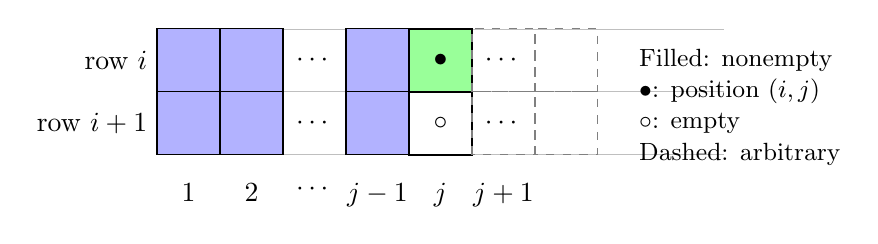
\begin{tikzpicture}[scale=0.8]
  % Draw grid
  \draw[lightgray, very thin] (0,0) -- (9,0);
  \draw[lightgray, very thin] (0,1) -- (9,1);
  \draw[lightgray, very thin] (0,2) -- (9,2);
  
  % Row i boxes - columns 1 and 2
  \foreach \x in {0,1} {
    \fill[blue!30] (\x,1) rectangle (\x+1,2);
    \draw (\x,1) rectangle (\x+1,2);
  }
  
  % Row i+1 boxes - columns 1 and 2
  \foreach \x in {0,1} {
    \fill[blue!30] (\x,0) rectangle (\x+1,1);
    \draw (\x,0) rectangle (\x+1,1);
  }
  
  % Ellipses between 2 and j-1
  \node at (2.5,1.5) {$\cdots$};
  \node at (2.5,0.5) {$\cdots$};
  
  % Column j-1
  \fill[blue!30] (3,1) rectangle (4,2);
  \draw (3,1) rectangle (4,2);
  \fill[blue!30] (3,0) rectangle (4,1);
  \draw (3,0) rectangle (4,1);
  
  % Position (i,j) - nonempty
  \fill[green!40] (4,1) rectangle (5,2);
  \draw[thick] (4,1) rectangle (5,2);
  \node at (4.5,1.5) {$\bullet$};
  
  % Position (i+1,j) - empty (white)
  \fill[white] (4,0) rectangle (5,1);
  \draw[thick] (4,0) rectangle (5,1);
  \node at (4.5,0.5) {$\circ$};
  
  % Visual ellipses for "anything can happen" to the right
  \draw[dashed, gray] (5,1) rectangle (6,2);
  \node at (5.5,1.5) {$\cdots$};
  \draw[dashed, gray] (5,0) rectangle (6,1);
  \node at (5.5,0.5) {$\cdots$};
  
  \draw[dashed, gray] (6,1) rectangle (7,2);
  \draw[dashed, gray] (6,0) rectangle (7,1);
  
  % Labels
  \node[left] at (0,1.5) {row $i$};
  \node[left] at (0,0.5) {row $i+1$};
  
  % Column labels
  \node[below] at (0.5,-0.3) {$1$};
  \node[below] at (1.5,-0.3) {$2$};
  \node[below] at (2.5,-0.3) {$\cdots$};
  \node[below] at (3.5,-0.3) {$j-1$};
  \node[below] at (4.5,-0.3) {$j$};
  \node[below] at (5.5,-0.3) {$j+1$};
  
  % Legend
  \node[anchor=west, align=left] at (7.5,1.5) {\small Filled: nonempty};
  \node[anchor=west, align=left] at (7.5,1) {\small $\bullet$: position $(i,j)$};
  \node[anchor=west, align=left] at (7.5,0.5) {\small $\circ$: empty};
  \node[anchor=west, align=left] at (7.5,0) {\small Dashed: arbitrary};
\end{tikzpicture}
\caption{Configuration for rows $i$ and $i+1$ for a ledge at $(i,j)$.}
\label{figure:ledge}
\end{figure}




\begin{theorem}
The crystal divided difference operators satisfy the relations:
$$\rcdd^i\rcdd^i = 0$$
$$\rcdd^i\rcdd^j = \rcdd^j\rcdd^i\quad\mbox{for }|i-j|>1$$
$$\rcdd^i\rcdd^{i+1}\rcdd^i = \rcdd^{i+1}\rcdd^i\rcdd^{i+1}$$
\end{theorem}

\begin{proof}
The first and second relations are not difficult. Otherwise, assume without loss of generality that $i=1$. For an RC graph with precisely three rows, let us consider applying $\rcdd^1\rcdd^2\rcdd^1$. Suppose $\code(w) = (a, b, c)$. It is well known that if $m=\min(a, b, c)$, then the first $m$ columns of $R$ are completely full, hence without loss of generality let us assume that $m=0$. The only way the braid relation can apply to yield a nonzero result, therefore, is if $a>b>c=0$. Since this yields a dominant permutation, it follows that $R$ is the unique RC graph for $w$. Applying the braid relation in either direction yields the complete sum of RC graphs for the permutation with code $(0, a - 1, b - 2)$ by application of Corollary \ref{corollary:generateschubert}. By transfer, this result also applies to the last two or three rows of any RC graph with respect to the code.

Considering a general RC graph, we may similarly assume that $\code_3(w)=0$ by removing full columns, since only ledges will yield nonzero results. If there are extra elements in the first three rows that are not in the implied dominant block, then they all satisfy $r + c - 1 > \code_r(w) + 1$, where $r\in \{1,2,3\}$ and the extra element is at row $(r,c)$, since they have come down from a row past row $4$ (with respect to the principal RC graph). Elements with $r + c - 1 > \code_1(w) + 1$ can be seen to have no essential interaction with rows $1$, $2$, and $3$ and can be disregarded. We are left with the configuration in Figure \ref{figure:whatsleft}.

In this situation, without ambiguity, application of the braid triple in either direction will delete the immobile $(2,1)$, $(1, \code_2(w) + 1)$, and $(1,1)$. Without application of any lowering operators, simply deleting these elements yields the highest weight of the crystal component containing $R$ with respect to the first three rows. Since we may apply $\clp^3(R)$ to obtain a Demazure crystal, the lowering operators transitively generate the sum. To see that we indeed get all of them, we note that for this highest weight $R' = \clp^3(R)$, application of $\rcdd^1\rcdd^2\rcdd^1$ should yield elements of the form
$$f_1^{a_1}f_2^{a_2}f_1^{a_3}R'$$
and for the other direction,
$$f_2^{b_1}f_1^{b_2}f_2^{b_3}R'$$
These are two distinct parametrizations of the Demazure crystal $B_{s_1s_2s_1}(\lambda)=B_{s_2s_1s_2}(\lambda)$ with highest weight $\lambda$, yielding the same elements.
\end{proof}


\newcommand{\BRF}{\mathcal{BRF}}
\newcommand{\RF}{\mathcal{RF}}
\newcommand{\cs}{\widetilde{s}}


\begin{figure}[h]
\centering
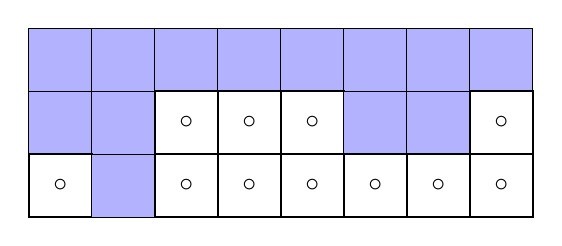
\begin{tikzpicture}[scale=0.8]
  % Row 1 (top row) - fully filled
  \fill[blue!30] (0,2) rectangle (1,3);
  \draw (0,2) rectangle (1,3);
  \fill[blue!30] (1,2) rectangle (2,3);
  \draw (1,2) rectangle (2,3);
  \fill[blue!30] (2,2) rectangle (3,3);
  \draw (2,2) rectangle (3,3);
  \fill[blue!30] (3,2) rectangle (4,3);
  \draw (3,2) rectangle (4,3);
  \fill[blue!30] (4,2) rectangle (5,3);
  \draw (4,2) rectangle (5,3);
  \fill[blue!30] (5,2) rectangle (6,3);
  \draw (5,2) rectangle (6,3);
  \fill[blue!30] (6,2) rectangle (7,3);
  \draw (6,2) rectangle (7,3);
  \fill[blue!30] (7,2) rectangle (8,3);
  \draw (7,2) rectangle (8,3);
  
  % Row 2 (middle row) - filled, empty, filled, empty
  \fill[blue!30] (0,1) rectangle (1,2);
  \draw (0,1) rectangle (1,2);
  \fill[blue!30] (1,1) rectangle (2,2);
  \draw (1,1) rectangle (2,2);
  \draw[thick] (2,1) rectangle (3,2);
  \node at (2.5,1.5) {$\circ$};
  \draw[thick] (3,1) rectangle (4,2);
  \node at (3.5,1.5) {$\circ$};
  \draw[thick] (4,1) rectangle (5,2);
  \node at (4.5,1.5) {$\circ$};
  \fill[blue!30] (5,1) rectangle (6,2);
  \draw (5,1) rectangle (6,2);
  \fill[blue!30] (6,1) rectangle (7,2);
  \draw (6,1) rectangle (7,2);
  \draw[thick] (7,1) rectangle (8,2);
  \node at (7.5,1.5) {$\circ$};
  
  % Row 3 (bottom row) - empty, filled, empty
  \draw[thick] (0,0) rectangle (1,1);
  \node at (0.5,0.5) {$\circ$};
  \fill[blue!30] (1,0) rectangle (2,1);
  \draw (1,0) rectangle (2,1);
  \draw[thick] (2,0) rectangle (3,1);
  \node at (2.5,0.5) {$\circ$};
  \draw[thick] (3,0) rectangle (4,1);
  \node at (3.5,0.5) {$\circ$};
  \draw[thick] (4,0) rectangle (5,1);
  \node at (4.5,0.5) {$\circ$};
  \draw[thick] (5,0) rectangle (6,1);
  \node at (5.5,0.5) {$\circ$};
  \draw[thick] (6,0) rectangle (7,1);
  \node at (6.5,0.5) {$\circ$};
  \draw[thick] (7,0) rectangle (8,1);
  \node at (7.5,0.5) {$\circ$};
  
\end{tikzpicture}
\caption{Configuration in the final steps of the proof of the braid relation.}
\label{figure:whatsleft}
\end{figure}



\begin{definition}
Let $R$ be an RC graph and let $p$ be an integer. Define $\clp^p(R)$ to be the RC graph obtained as follows. Let $R_{\leq p}$ be the subgraph of $R$ consisting of rows $1,2,\ldots,p$, and suppose $\maxd(\wof{R_{\leq p}}) = p + m$. If $m\leq 0$, set $\clp^p(R) = R_{\leq p}$. Otherwise, define
$$\clp^p(R) = \zeromap^m(R_{\leq p}, p + m)$$
Also, we define $\trm^p(R)$ as
$$\trm^p(R) = \{(i - p, j) \mid (i, j)\in R, i > p\}$$
\end{definition}

\begin{definition}[The natural map $\mathcal{U}_i:\BRC(s_iw, n)\to \BRC(w,n)$]
Suppose $R_1, R_2$ are RC graphs and $s_i$ is a left descent of $\wof{R_1}$. Then $I(R_2)\subseteq I(R_1)$, and hence the inclusion $R_2\hookrightarrow R_1$ preserves right inversions. We can turn this into a canonical map 
$$\mathcal{U}_i:\BRC(s_iw, n)\to \BRC(w,n)$$
by choosing $R_1$ to be the unique RC graph in $\BRC(w,n)$ such that $R_2^T$ has a nonzero coefficient in $\rcdd^i(R_1^T)$ (which exists by Lemma \ref{lemma:divdiffunique} and Theorem \ref{theorem:divdiffschubert}).
\end{definition}

\begin{theorem} \label{theorem:commutative_diagram}
Let $w\in S_\infty$ satisfy $\maxd(w)\leq n$ and suppose $i$ is a left descent of $w$. Then we have a commutative diagram
\[
\begin{tikzcd}
\BRC(s_iw, n) \arrow[r, "\clp^{n-1}"] \arrow[d, "\mathcal{U}_i"] & \displaystyle\bigcup_{s_iw\downvar{n} s_iw'}\BRC(s_iw', n-1) \arrow[d, "\mathcal{U}_i"] \\
\BRC(w, n) \arrow[r, "\clp^{n-1}"] & \displaystyle\bigcup_{w\downvar{n} w'}\BRC(w', n-1)
\end{tikzcd}
\]
\end{theorem}


\begin{lemma} \label{lemma:assoc_clip}
  We have the following equations for an RC graph $R$ and two integers $p$ and $q$:
$$\clp^p(\clp^{p+q}(R)) = \clp^p(R)$$
$$\trm^p(\clp^{p+q}(R)) = \clp^q(\trm^p(R))$$ 
and 
$$\trm^{p+q}(R) = \trm^q(\trm^{p}(R))$$
\end{lemma}
\begin{proof}
Suppose $(R, n)$ is a bounded RC graph. We prove that $\clp^{n-2}(\clp^{n-1}(R)) = \clp^{n-2}(R)$. For $n=2$, this is trivial. As an additional base case, we also need $n=3$, which is not trivial, but true because a bounded RC graph $(R,1)$ is uniquely determined by its size. We proceed by induction on $n$. Without loss of generality, assume that row $n$ is empty. Then $\clp^{n-1}(R) = \zeromap(R)$. We have
$$\clp^{n-2}(R) = \zeromap^2(R_{\leq n-2}, n)=\zeromap(\zeromap(R_{\leq n-2}))$$
$$\clp^{n-2}(\clp^{n-1}(R)) = \zeromap(\zeromap(R)_{\leq n-2}, n-1)$$
IF $\maxd(\wof{R_{\leq n-2}})\leq n-1$, then both sides are equal to $\zeromap(R_{\leq n-2})$. Otherwise, by Lemma \ref{lemma:ztrim}, we have
$$\trm(\clp^{n-2}(R)) = \trm(\zeromap(\zeromap(R_{\leq n-2}))) =\zeromap(\zeromap(\trm(R)_{\leq n-3}))$$
$$\trm(\clp^{n-2}(\clp^{n-1}(R))) = \zeromap(\zeromap(\trm(R))_{\leq n-3}, n-2)$$
Thus, $\clp^{n-2}(\clp^{n-1}(R))$ and $\clp^{n-2}(R)$ agree on all rows except possibly the first row. We proceed by induction on the number of elements of $R$ in the first row. For zero elements, the result is obvious. If we have proved the result for $k-1$ elements in the first row, let $(1, i)$ be the rightmost such element. Then $R\setminus\{(1,i)\}$ has $k-1$ elements in the first row, so by the inductive hypothesis, $\clp^{n-2}(\clp^{n-1}(R\setminus\{(1,i)\})) = \clp^{n-2}(R\setminus\{(1,i)\})$. Applying Theorem \ref{theorem:commutative_diagram}, we see that adding back in the element $(1,i)$ to both sides preserves equality, due to the commutativity of the diagram. This establishes the first equation. The second equation easily follows from repeated application of Lemma \ref{lemma:ztrim}, and the third equation is the definition of $\trm$.
\end{proof}

\begin{theorem} \label{theorem:howyouslice}
  Let $r>0$ be an integer and suppose $p\geq 0$ is an integer such that $p\leq r$. Then the map $\BRC(r)\to \BRC(p)\times \BRC(r - p)\times S_\infty$ defined by
  $$(R, r)\mapsto (\clp^p(R, r), \trm^{p}(R, r), \wof{R})$$
  is injective.
\end{theorem}
\begin{proof}
For $p = 0$ this is trivial, and for $p = 1$ this is due to the fact that any subset of the first row of an RC graph corresponds to a unique permutation, so that if we know $\trm^1(R, r) = (R', r - 1)$ and we know $\wof{R}$, then $R$ is the unique RC graph such that the first row corresponds to the permutation $u$ such that $u\wof{R'}=\wof{R}$ and $\trm^1(R, r) = (R', r-1)$. 

For $p=r-1$, we use the fact that row $r$ of a bounded RC graph $(R,r)$ is uniquely determined by its weight. It therefore suffices to prove the result when this weight is $0$, which is covered by Theorem \ref{theorem:zero_bijection}. We have thus proved the theorem for $r=2$.

For larger $r$, we prove the result by induction on $p$, keeping in mind the solutions for the cases $p=0,1,r-1$. We know that $(R,r)$ is uniquely determined by $(\clp^{r-1}(R), \wof{R})$ and we may use the inductive hypothesis to reason that it is therefore uniquely determined by $(\clp^{p}(R), \trm^p(\clp^{r-1}(R)), \wof{R})$. Furthermore, Let $u=\wof{\clp^{p}(R)}$. Then the pair $(\trm^{p-1}(\clp^{r-1}(R)), u^{-1}\wof{R})$ uniquely determines $\trm^p(R)$ by the inductive hypothesis. Hence $(\clp^{p}(R), \trm^{p}(R), \wof{R})$ uniquely determines $(R, r)$, establishing injectivity.
\end{proof}

\subsection{Definition of the ring product}

\begin{definition}
Suppose we have two bounded RC graphs $R_1$ with $\hr(R_1)=m$ and $R_2$ with $\hr(R_2)=n$. The product of these is defined by
$$R_1\diamond R_2 = \sum_{\substack{\clp^m(R')=R_1\\\trm^m(R')=R_2}}R'$$  
where $R'$ ranges over bounded RC graphs with $\hr(R')=m+n$.

Define a map $D:\BRC\to \dcoma\otimes \dcoma$ by
$$D(R) = \dsch_{\wof{R}}^{\hr(R)}\otimes [\wtt(R)]$$
\end{definition}

\begin{theorem}
	 The product $\diamond$ turns $\BRC$ into a ring, and $D:\BRC\to \dcoma\otimes \dcoma$ is a homomorphism of rings.
\end{theorem}
\begin{proof}
What is in question is associativity. Suppose we have three bounded RC graphs $R_1$ with $\hr(R_1)=p$, $R_2$ with $\hr(R_2)=q$, and $R_3$ with $\hr(R_3)=r$, and we want to show that the order of bracketing the product is irrelevant. This is because if $R_w$ is a term in the expansion of the product with $\hr(R_w)=p+q+r$, then
$$\clp^p(\clp^{p+q}(R_w)) = R_1 = \clp^p(R_w)$$
$$\trm^p(\clp^{p+q}(R_w)) = R_2 = \clp^q(\trm^p(R_w))$$ 
and 
$$\trm^{p+q}(R_w) = R_3 = \trm^q(\trm^{p}(R_w))$$
by Lemma \ref{lemma:assoc_clip}, and each term in the expansion of the product has a coefficient of $1$.

To prove the map $D:\BRC\to \dcoma\otimes \dcoma$ is a homomorphism of rings, we utilize the formula for the coefficient $d_{u,v}^w(p,q)$ as the coefficient of $\sch_u(x_1,\ldots,x_p)$ when we set $x_{p+1}=\cdots=x_{p+q}=0$ in the polynomial
$$\partial^{\shup^p v}\sch_w(x_1,\ldots,x_{p+q})$$
(that is, Theorem \ref{theorem:LRdual}). We claim that if we fix an RC graph $R_u$ for $u$ and an RC graph $R_v$ for $v$, then this coefficient is the same as the number of BRCs $(R, p+q)$ for $w$ such that $\trm^p(R)=R_v$ and $\clp^p(R) = R_u$. If we assume that $v$ is the identity, this follows from Theorem \ref{theorem:transition} and Theorem \ref{theorem:zero_bijection}. The divided difference operator characterization means that for $\ell(v)>0$, we can replace the empty space with any (shifted up) RC graph for $v$ $(R_v, q)$ and get the result for $\alpha$ as desired. Since the weight is also preserved in this construction, the result follows for $D$ as well.
\end{proof}

%We would also like a combinatorial interpretation of this product.
BPD FROM BRUHAT MODULE

\begin{example}
We compute the product of two bounded RC graphs $(R_1, 2)\in\BRC(2413,2)$ and $(R_2, 2)\in\BRC(231,2)$:
\begin{align*}
  &
  \vcenter{\hbox{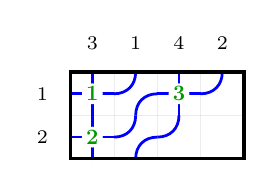
\begin{tikzpicture}[scale=0.55]
  \draw[lightgray, very thin, opacity=0.3] (0,2) -- (4,2);
  \draw[lightgray, very thin, opacity=0.3] (0,3) -- (4,3);
  \draw[lightgray, very thin, opacity=0.3] (0,4) -- (4,4);
  \draw[lightgray, very thin, opacity=0.3] (0,2) -- (0,4);
  \draw[lightgray, very thin, opacity=0.3] (1,2) -- (1,4);
  \draw[lightgray, very thin, opacity=0.3] (2,2) -- (2,4);
  \draw[lightgray, very thin, opacity=0.3] (3,2) -- (3,4);
  \draw[lightgray, very thin, opacity=0.3] (4,2) -- (4,4);
  \draw[blue, line width=1.0pt, line cap=round] (0,3.5) -- (1,3.5);
  \draw[blue, line width=1.0pt, line cap=round] (0.5,3) -- (0.5,4);
  \draw[blue, line width=1.0pt] (1,3.5) .. controls (1.3,3.5) and (1.5,3.7) .. (1.5,4);
  \draw[blue, line width=1.0pt] (1.5,3) .. controls (1.5,3.3) and (1.7,3.5) .. (2,3.5);
  \draw[blue, line width=1.0pt, line cap=round] (2,3.5) -- (3,3.5);
  \draw[blue, line width=1.0pt, line cap=round] (2.5,3) -- (2.5,4);
  \draw[blue, line width=1.0pt] (3,3.5) .. controls (3.3,3.5) and (3.5,3.7) .. (3.5,4);
  \draw[blue, line width=1.0pt, line cap=round] (0,2.5) -- (1,2.5);
  \draw[blue, line width=1.0pt, line cap=round] (0.5,2) -- (0.5,3);
  \draw[blue, line width=1.0pt] (1,2.5) .. controls (1.3,2.5) and (1.5,2.7) .. (1.5,3);
  \draw[blue, line width=1.0pt] (1.5,2) .. controls (1.5,2.3) and (1.7,2.5) .. (2,2.5);
  \draw[blue, line width=1.0pt] (2,2.5) .. controls (2.3,2.5) and (2.5,2.7) .. (2.5,3);
  \node[font=\Large\bfseries, text=green!60!black, fill=white, inner sep=0.5pt, circle, transform shape] at (0.5,3.5) {1};
  \node[font=\Large\bfseries, text=green!60!black, fill=white, inner sep=0.5pt, circle, transform shape] at (2.5,3.5) {3};
  \node[font=\Large\bfseries, text=green!60!black, fill=white, inner sep=0.5pt, circle, transform shape] at (0.5,2.5) {2};
  \node[font=\scriptsize, text=black, anchor=south] at (0.5,4.3) {3};
  \node[font=\scriptsize, text=black, anchor=south] at (1.5,4.3) {1};
  \node[font=\scriptsize, text=black, anchor=south] at (2.5,4.3) {4};
  \node[font=\scriptsize, text=black, anchor=south] at (3.5,4.3) {2};
  \node[font=\scriptsize, text=black, anchor=east] at (-0.3,3.5) {1};
  \node[font=\scriptsize, text=black, anchor=east] at (-0.3,2.5) {2};
  \draw[black, line width=1.2000000000000002pt] (0,2) rectangle (4,4);
\end{tikzpicture}}}
  \diamond
  \vcenter{\hbox{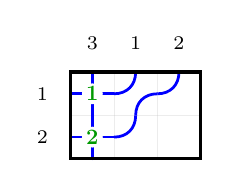
\begin{tikzpicture}[scale=0.55]
  \draw[lightgray, very thin, opacity=0.3] (0,1) -- (3,1);
  \draw[lightgray, very thin, opacity=0.3] (0,2) -- (3,2);
  \draw[lightgray, very thin, opacity=0.3] (0,3) -- (3,3);
  \draw[lightgray, very thin, opacity=0.3] (0,1) -- (0,3);
  \draw[lightgray, very thin, opacity=0.3] (1,1) -- (1,3);
  \draw[lightgray, very thin, opacity=0.3] (2,1) -- (2,3);
  \draw[lightgray, very thin, opacity=0.3] (3,1) -- (3,3);
  \draw[blue, line width=1.0pt, line cap=round] (0,2.5) -- (1,2.5);
  \draw[blue, line width=1.0pt, line cap=round] (0.5,2) -- (0.5,3);
  \draw[blue, line width=1.0pt] (1,2.5) .. controls (1.3,2.5) and (1.5,2.7) .. (1.5,3);
  \draw[blue, line width=1.0pt] (1.5,2) .. controls (1.5,2.3) and (1.7,2.5) .. (2,2.5);
  \draw[blue, line width=1.0pt] (2,2.5) .. controls (2.3,2.5) and (2.5,2.7) .. (2.5,3);
  \draw[blue, line width=1.0pt, line cap=round] (0,1.5) -- (1,1.5);
  \draw[blue, line width=1.0pt, line cap=round] (0.5,1) -- (0.5,2);
  \draw[blue, line width=1.0pt] (1,1.5) .. controls (1.3,1.5) and (1.5,1.7) .. (1.5,2);
  \node[font=\Large\bfseries, text=green!60!black, fill=white, inner sep=0.5pt, circle, transform shape] at (0.5,2.5) {1};
  \node[font=\Large\bfseries, text=green!60!black, fill=white, inner sep=0.5pt, circle, transform shape] at (0.5,1.5) {2};
  \node[font=\scriptsize, text=black, anchor=south] at (0.5,3.3) {3};
  \node[font=\scriptsize, text=black, anchor=south] at (1.5,3.3) {1};
  \node[font=\scriptsize, text=black, anchor=south] at (2.5,3.3) {2};
  \node[font=\scriptsize, text=black, anchor=east] at (-0.3,2.5) {1};
  \node[font=\scriptsize, text=black, anchor=east] at (-0.3,1.5) {2};
  \draw[black, line width=1.2000000000000002pt] (0,1) rectangle (3,3);
\end{tikzpicture}}}
  \\[1em]
  ={}& 
  \vcenter{\hbox{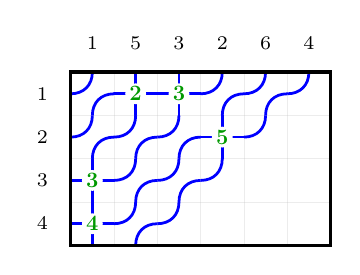
\begin{tikzpicture}[scale=0.55]
  \draw[lightgray, very thin, opacity=0.3] (0,2) -- (6,2);
  \draw[lightgray, very thin, opacity=0.3] (0,3) -- (6,3);
  \draw[lightgray, very thin, opacity=0.3] (0,4) -- (6,4);
  \draw[lightgray, very thin, opacity=0.3] (0,5) -- (6,5);
  \draw[lightgray, very thin, opacity=0.3] (0,6) -- (6,6);
  \draw[lightgray, very thin, opacity=0.3] (0,2) -- (0,6);
  \draw[lightgray, very thin, opacity=0.3] (1,2) -- (1,6);
  \draw[lightgray, very thin, opacity=0.3] (2,2) -- (2,6);
  \draw[lightgray, very thin, opacity=0.3] (3,2) -- (3,6);
  \draw[lightgray, very thin, opacity=0.3] (4,2) -- (4,6);
  \draw[lightgray, very thin, opacity=0.3] (5,2) -- (5,6);
  \draw[lightgray, very thin, opacity=0.3] (6,2) -- (6,6);
  \draw[blue, line width=1.0pt] (0,5.5) .. controls (0.3,5.5) and (0.5,5.7) .. (0.5,6);
  \draw[blue, line width=1.0pt] (0.5,5) .. controls (0.5,5.3) and (0.7,5.5) .. (1,5.5);
  \draw[blue, line width=1.0pt, line cap=round] (1,5.5) -- (2,5.5);
  \draw[blue, line width=1.0pt, line cap=round] (1.5,5) -- (1.5,6);
  \draw[blue, line width=1.0pt, line cap=round] (2,5.5) -- (3,5.5);
  \draw[blue, line width=1.0pt, line cap=round] (2.5,5) -- (2.5,6);
  \draw[blue, line width=1.0pt] (3,5.5) .. controls (3.3,5.5) and (3.5,5.7) .. (3.5,6);
  \draw[blue, line width=1.0pt] (3.5,5) .. controls (3.5,5.3) and (3.7,5.5) .. (4,5.5);
  \draw[blue, line width=1.0pt] (4,5.5) .. controls (4.3,5.5) and (4.5,5.7) .. (4.5,6);
  \draw[blue, line width=1.0pt] (4.5,5) .. controls (4.5,5.3) and (4.7,5.5) .. (5,5.5);
  \draw[blue, line width=1.0pt] (5,5.5) .. controls (5.3,5.5) and (5.5,5.7) .. (5.5,6);
  \draw[blue, line width=1.0pt] (0,4.5) .. controls (0.3,4.5) and (0.5,4.7) .. (0.5,5);
  \draw[blue, line width=1.0pt] (0.5,4) .. controls (0.5,4.3) and (0.7,4.5) .. (1,4.5);
  \draw[blue, line width=1.0pt] (1,4.5) .. controls (1.3,4.5) and (1.5,4.7) .. (1.5,5);
  \draw[blue, line width=1.0pt] (1.5,4) .. controls (1.5,4.3) and (1.7,4.5) .. (2,4.5);
  \draw[blue, line width=1.0pt] (2,4.5) .. controls (2.3,4.5) and (2.5,4.7) .. (2.5,5);
  \draw[blue, line width=1.0pt] (2.5,4) .. controls (2.5,4.3) and (2.7,4.5) .. (3,4.5);
  \draw[blue, line width=1.0pt, line cap=round] (3,4.5) -- (4,4.5);
  \draw[blue, line width=1.0pt, line cap=round] (3.5,4) -- (3.5,5);
  \draw[blue, line width=1.0pt] (4,4.5) .. controls (4.3,4.5) and (4.5,4.7) .. (4.5,5);
  \draw[blue, line width=1.0pt, line cap=round] (0,3.5) -- (1,3.5);
  \draw[blue, line width=1.0pt, line cap=round] (0.5,3) -- (0.5,4);
  \draw[blue, line width=1.0pt] (1,3.5) .. controls (1.3,3.5) and (1.5,3.7) .. (1.5,4);
  \draw[blue, line width=1.0pt] (1.5,3) .. controls (1.5,3.3) and (1.7,3.5) .. (2,3.5);
  \draw[blue, line width=1.0pt] (2,3.5) .. controls (2.3,3.5) and (2.5,3.7) .. (2.5,4);
  \draw[blue, line width=1.0pt] (2.5,3) .. controls (2.5,3.3) and (2.7,3.5) .. (3,3.5);
  \draw[blue, line width=1.0pt] (3,3.5) .. controls (3.3,3.5) and (3.5,3.7) .. (3.5,4);
  \draw[blue, line width=1.0pt, line cap=round] (0,2.5) -- (1,2.5);
  \draw[blue, line width=1.0pt, line cap=round] (0.5,2) -- (0.5,3);
  \draw[blue, line width=1.0pt] (1,2.5) .. controls (1.3,2.5) and (1.5,2.7) .. (1.5,3);
  \draw[blue, line width=1.0pt] (1.5,2) .. controls (1.5,2.3) and (1.7,2.5) .. (2,2.5);
  \draw[blue, line width=1.0pt] (2,2.5) .. controls (2.3,2.5) and (2.5,2.7) .. (2.5,3);
  \node[font=\Large\bfseries, text=green!60!black, fill=white, inner sep=0.5pt, circle, transform shape] at (3.5,4.5) {5};
  \node[font=\Large\bfseries, text=green!60!black, fill=white, inner sep=0.5pt, circle, transform shape] at (1.5,5.5) {2};
  \node[font=\Large\bfseries, text=green!60!black, fill=white, inner sep=0.5pt, circle, transform shape] at (0.5,2.5) {4};
  \node[font=\Large\bfseries, text=green!60!black, fill=white, inner sep=0.5pt, circle, transform shape] at (0.5,3.5) {3};
  \node[font=\Large\bfseries, text=green!60!black, fill=white, inner sep=0.5pt, circle, transform shape] at (2.5,5.5) {3};
  \node[font=\scriptsize, text=black, anchor=south] at (0.5,6.3) {1};
  \node[font=\scriptsize, text=black, anchor=south] at (1.5,6.3) {5};
  \node[font=\scriptsize, text=black, anchor=south] at (2.5,6.3) {3};
  \node[font=\scriptsize, text=black, anchor=south] at (3.5,6.3) {2};
  \node[font=\scriptsize, text=black, anchor=south] at (4.5,6.3) {6};
  \node[font=\scriptsize, text=black, anchor=south] at (5.5,6.3) {4};
  \node[font=\scriptsize, text=black, anchor=east] at (-0.3,5.5) {1};
  \node[font=\scriptsize, text=black, anchor=east] at (-0.3,4.5) {2};
  \node[font=\scriptsize, text=black, anchor=east] at (-0.3,3.5) {3};
  \node[font=\scriptsize, text=black, anchor=east] at (-0.3,2.5) {4};
  \draw[black, line width=1.2000000000000002pt] (0,2) rectangle (6,6);
\end{tikzpicture}}}
  +
  \vcenter{\hbox{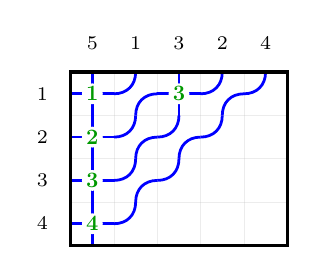
\begin{tikzpicture}[scale=0.55]
  \draw[lightgray, very thin, opacity=0.3] (0,1) -- (5,1);
  \draw[lightgray, very thin, opacity=0.3] (0,2) -- (5,2);
  \draw[lightgray, very thin, opacity=0.3] (0,3) -- (5,3);
  \draw[lightgray, very thin, opacity=0.3] (0,4) -- (5,4);
  \draw[lightgray, very thin, opacity=0.3] (0,5) -- (5,5);
  \draw[lightgray, very thin, opacity=0.3] (0,1) -- (0,5);
  \draw[lightgray, very thin, opacity=0.3] (1,1) -- (1,5);
  \draw[lightgray, very thin, opacity=0.3] (2,1) -- (2,5);
  \draw[lightgray, very thin, opacity=0.3] (3,1) -- (3,5);
  \draw[lightgray, very thin, opacity=0.3] (4,1) -- (4,5);
  \draw[lightgray, very thin, opacity=0.3] (5,1) -- (5,5);
  \draw[blue, line width=1.0pt, line cap=round] (0,4.5) -- (1,4.5);
  \draw[blue, line width=1.0pt, line cap=round] (0.5,4) -- (0.5,5);
  \draw[blue, line width=1.0pt] (1,4.5) .. controls (1.3,4.5) and (1.5,4.7) .. (1.5,5);
  \draw[blue, line width=1.0pt] (1.5,4) .. controls (1.5,4.3) and (1.7,4.5) .. (2,4.5);
  \draw[blue, line width=1.0pt, line cap=round] (2,4.5) -- (3,4.5);
  \draw[blue, line width=1.0pt, line cap=round] (2.5,4) -- (2.5,5);
  \draw[blue, line width=1.0pt] (3,4.5) .. controls (3.3,4.5) and (3.5,4.7) .. (3.5,5);
  \draw[blue, line width=1.0pt] (3.5,4) .. controls (3.5,4.3) and (3.7,4.5) .. (4,4.5);
  \draw[blue, line width=1.0pt] (4,4.5) .. controls (4.3,4.5) and (4.5,4.7) .. (4.5,5);
  \draw[blue, line width=1.0pt, line cap=round] (0,3.5) -- (1,3.5);
  \draw[blue, line width=1.0pt, line cap=round] (0.5,3) -- (0.5,4);
  \draw[blue, line width=1.0pt] (1,3.5) .. controls (1.3,3.5) and (1.5,3.7) .. (1.5,4);
  \draw[blue, line width=1.0pt] (1.5,3) .. controls (1.5,3.3) and (1.7,3.5) .. (2,3.5);
  \draw[blue, line width=1.0pt] (2,3.5) .. controls (2.3,3.5) and (2.5,3.7) .. (2.5,4);
  \draw[blue, line width=1.0pt] (2.5,3) .. controls (2.5,3.3) and (2.7,3.5) .. (3,3.5);
  \draw[blue, line width=1.0pt] (3,3.5) .. controls (3.3,3.5) and (3.5,3.7) .. (3.5,4);
  \draw[blue, line width=1.0pt, line cap=round] (0,2.5) -- (1,2.5);
  \draw[blue, line width=1.0pt, line cap=round] (0.5,2) -- (0.5,3);
  \draw[blue, line width=1.0pt] (1,2.5) .. controls (1.3,2.5) and (1.5,2.7) .. (1.5,3);
  \draw[blue, line width=1.0pt] (1.5,2) .. controls (1.5,2.3) and (1.7,2.5) .. (2,2.5);
  \draw[blue, line width=1.0pt] (2,2.5) .. controls (2.3,2.5) and (2.5,2.7) .. (2.5,3);
  \draw[blue, line width=1.0pt, line cap=round] (0,1.5) -- (1,1.5);
  \draw[blue, line width=1.0pt, line cap=round] (0.5,1) -- (0.5,2);
  \draw[blue, line width=1.0pt] (1,1.5) .. controls (1.3,1.5) and (1.5,1.7) .. (1.5,2);
  \node[font=\Large\bfseries, text=green!60!black, fill=white, inner sep=0.5pt, circle, transform shape] at (0.5,3.5) {2};
  \node[font=\Large\bfseries, text=green!60!black, fill=white, inner sep=0.5pt, circle, transform shape] at (0.5,1.5) {4};
  \node[font=\Large\bfseries, text=green!60!black, fill=white, inner sep=0.5pt, circle, transform shape] at (0.5,2.5) {3};
  \node[font=\Large\bfseries, text=green!60!black, fill=white, inner sep=0.5pt, circle, transform shape] at (0.5,4.5) {1};
  \node[font=\Large\bfseries, text=green!60!black, fill=white, inner sep=0.5pt, circle, transform shape] at (2.5,4.5) {3};
  \node[font=\scriptsize, text=black, anchor=south] at (0.5,5.3) {5};
  \node[font=\scriptsize, text=black, anchor=south] at (1.5,5.3) {1};
  \node[font=\scriptsize, text=black, anchor=south] at (2.5,5.3) {3};
  \node[font=\scriptsize, text=black, anchor=south] at (3.5,5.3) {2};
  \node[font=\scriptsize, text=black, anchor=south] at (4.5,5.3) {4};
  \node[font=\scriptsize, text=black, anchor=east] at (-0.3,4.5) {1};
  \node[font=\scriptsize, text=black, anchor=east] at (-0.3,3.5) {2};
  \node[font=\scriptsize, text=black, anchor=east] at (-0.3,2.5) {3};
  \node[font=\scriptsize, text=black, anchor=east] at (-0.3,1.5) {4};
  \draw[black, line width=1.2000000000000002pt] (0,1) rectangle (5,5);
\end{tikzpicture}}}
  +
  \vcenter{\hbox{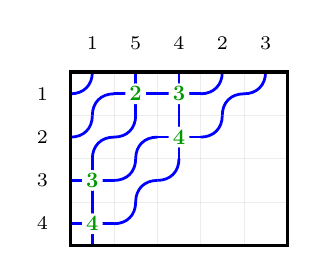
\begin{tikzpicture}[scale=0.55]
  \draw[lightgray, very thin, opacity=0.3] (0,1) -- (5,1);
  \draw[lightgray, very thin, opacity=0.3] (0,2) -- (5,2);
  \draw[lightgray, very thin, opacity=0.3] (0,3) -- (5,3);
  \draw[lightgray, very thin, opacity=0.3] (0,4) -- (5,4);
  \draw[lightgray, very thin, opacity=0.3] (0,5) -- (5,5);
  \draw[lightgray, very thin, opacity=0.3] (0,1) -- (0,5);
  \draw[lightgray, very thin, opacity=0.3] (1,1) -- (1,5);
  \draw[lightgray, very thin, opacity=0.3] (2,1) -- (2,5);
  \draw[lightgray, very thin, opacity=0.3] (3,1) -- (3,5);
  \draw[lightgray, very thin, opacity=0.3] (4,1) -- (4,5);
  \draw[lightgray, very thin, opacity=0.3] (5,1) -- (5,5);
  \draw[blue, line width=1.0pt] (0,4.5) .. controls (0.3,4.5) and (0.5,4.7) .. (0.5,5);
  \draw[blue, line width=1.0pt] (0.5,4) .. controls (0.5,4.3) and (0.7,4.5) .. (1,4.5);
  \draw[blue, line width=1.0pt, line cap=round] (1,4.5) -- (2,4.5);
  \draw[blue, line width=1.0pt, line cap=round] (1.5,4) -- (1.5,5);
  \draw[blue, line width=1.0pt, line cap=round] (2,4.5) -- (3,4.5);
  \draw[blue, line width=1.0pt, line cap=round] (2.5,4) -- (2.5,5);
  \draw[blue, line width=1.0pt] (3,4.5) .. controls (3.3,4.5) and (3.5,4.7) .. (3.5,5);
  \draw[blue, line width=1.0pt] (3.5,4) .. controls (3.5,4.3) and (3.7,4.5) .. (4,4.5);
  \draw[blue, line width=1.0pt] (4,4.5) .. controls (4.3,4.5) and (4.5,4.7) .. (4.5,5);
  \draw[blue, line width=1.0pt] (0,3.5) .. controls (0.3,3.5) and (0.5,3.7) .. (0.5,4);
  \draw[blue, line width=1.0pt] (0.5,3) .. controls (0.5,3.3) and (0.7,3.5) .. (1,3.5);
  \draw[blue, line width=1.0pt] (1,3.5) .. controls (1.3,3.5) and (1.5,3.7) .. (1.5,4);
  \draw[blue, line width=1.0pt] (1.5,3) .. controls (1.5,3.3) and (1.7,3.5) .. (2,3.5);
  \draw[blue, line width=1.0pt, line cap=round] (2,3.5) -- (3,3.5);
  \draw[blue, line width=1.0pt, line cap=round] (2.5,3) -- (2.5,4);
  \draw[blue, line width=1.0pt] (3,3.5) .. controls (3.3,3.5) and (3.5,3.7) .. (3.5,4);
  \draw[blue, line width=1.0pt, line cap=round] (0,2.5) -- (1,2.5);
  \draw[blue, line width=1.0pt, line cap=round] (0.5,2) -- (0.5,3);
  \draw[blue, line width=1.0pt] (1,2.5) .. controls (1.3,2.5) and (1.5,2.7) .. (1.5,3);
  \draw[blue, line width=1.0pt] (1.5,2) .. controls (1.5,2.3) and (1.7,2.5) .. (2,2.5);
  \draw[blue, line width=1.0pt] (2,2.5) .. controls (2.3,2.5) and (2.5,2.7) .. (2.5,3);
  \draw[blue, line width=1.0pt, line cap=round] (0,1.5) -- (1,1.5);
  \draw[blue, line width=1.0pt, line cap=round] (0.5,1) -- (0.5,2);
  \draw[blue, line width=1.0pt] (1,1.5) .. controls (1.3,1.5) and (1.5,1.7) .. (1.5,2);
  \node[font=\Large\bfseries, text=green!60!black, fill=white, inner sep=0.5pt, circle, transform shape] at (1.5,4.5) {2};
  \node[font=\Large\bfseries, text=green!60!black, fill=white, inner sep=0.5pt, circle, transform shape] at (0.5,1.5) {4};
  \node[font=\Large\bfseries, text=green!60!black, fill=white, inner sep=0.5pt, circle, transform shape] at (0.5,2.5) {3};
  \node[font=\Large\bfseries, text=green!60!black, fill=white, inner sep=0.5pt, circle, transform shape] at (2.5,3.5) {4};
  \node[font=\Large\bfseries, text=green!60!black, fill=white, inner sep=0.5pt, circle, transform shape] at (2.5,4.5) {3};
  \node[font=\scriptsize, text=black, anchor=south] at (0.5,5.3) {1};
  \node[font=\scriptsize, text=black, anchor=south] at (1.5,5.3) {5};
  \node[font=\scriptsize, text=black, anchor=south] at (2.5,5.3) {4};
  \node[font=\scriptsize, text=black, anchor=south] at (3.5,5.3) {2};
  \node[font=\scriptsize, text=black, anchor=south] at (4.5,5.3) {3};
  \node[font=\scriptsize, text=black, anchor=east] at (-0.3,4.5) {1};
  \node[font=\scriptsize, text=black, anchor=east] at (-0.3,3.5) {2};
  \node[font=\scriptsize, text=black, anchor=east] at (-0.3,2.5) {3};
  \node[font=\scriptsize, text=black, anchor=east] at (-0.3,1.5) {4};
  \draw[black, line width=1.2000000000000002pt] (0,1) rectangle (5,5);
\end{tikzpicture}}}
  \\[1em]
  + & 
  \vcenter{\hbox{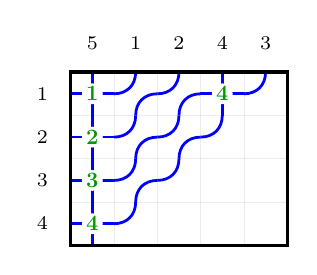
\begin{tikzpicture}[scale=0.55]
  \draw[lightgray, very thin, opacity=0.3] (0,1) -- (5,1);
  \draw[lightgray, very thin, opacity=0.3] (0,2) -- (5,2);
  \draw[lightgray, very thin, opacity=0.3] (0,3) -- (5,3);
  \draw[lightgray, very thin, opacity=0.3] (0,4) -- (5,4);
  \draw[lightgray, very thin, opacity=0.3] (0,5) -- (5,5);
  \draw[lightgray, very thin, opacity=0.3] (0,1) -- (0,5);
  \draw[lightgray, very thin, opacity=0.3] (1,1) -- (1,5);
  \draw[lightgray, very thin, opacity=0.3] (2,1) -- (2,5);
  \draw[lightgray, very thin, opacity=0.3] (3,1) -- (3,5);
  \draw[lightgray, very thin, opacity=0.3] (4,1) -- (4,5);
  \draw[lightgray, very thin, opacity=0.3] (5,1) -- (5,5);
  \draw[blue, line width=1.0pt, line cap=round] (0,4.5) -- (1,4.5);
  \draw[blue, line width=1.0pt, line cap=round] (0.5,4) -- (0.5,5);
  \draw[blue, line width=1.0pt] (1,4.5) .. controls (1.3,4.5) and (1.5,4.7) .. (1.5,5);
  \draw[blue, line width=1.0pt] (1.5,4) .. controls (1.5,4.3) and (1.7,4.5) .. (2,4.5);
  \draw[blue, line width=1.0pt] (2,4.5) .. controls (2.3,4.5) and (2.5,4.7) .. (2.5,5);
  \draw[blue, line width=1.0pt] (2.5,4) .. controls (2.5,4.3) and (2.7,4.5) .. (3,4.5);
  \draw[blue, line width=1.0pt, line cap=round] (3,4.5) -- (4,4.5);
  \draw[blue, line width=1.0pt, line cap=round] (3.5,4) -- (3.5,5);
  \draw[blue, line width=1.0pt] (4,4.5) .. controls (4.3,4.5) and (4.5,4.7) .. (4.5,5);
  \draw[blue, line width=1.0pt, line cap=round] (0,3.5) -- (1,3.5);
  \draw[blue, line width=1.0pt, line cap=round] (0.5,3) -- (0.5,4);
  \draw[blue, line width=1.0pt] (1,3.5) .. controls (1.3,3.5) and (1.5,3.7) .. (1.5,4);
  \draw[blue, line width=1.0pt] (1.5,3) .. controls (1.5,3.3) and (1.7,3.5) .. (2,3.5);
  \draw[blue, line width=1.0pt] (2,3.5) .. controls (2.3,3.5) and (2.5,3.7) .. (2.5,4);
  \draw[blue, line width=1.0pt] (2.5,3) .. controls (2.5,3.3) and (2.7,3.5) .. (3,3.5);
  \draw[blue, line width=1.0pt] (3,3.5) .. controls (3.3,3.5) and (3.5,3.7) .. (3.5,4);
  \draw[blue, line width=1.0pt, line cap=round] (0,2.5) -- (1,2.5);
  \draw[blue, line width=1.0pt, line cap=round] (0.5,2) -- (0.5,3);
  \draw[blue, line width=1.0pt] (1,2.5) .. controls (1.3,2.5) and (1.5,2.7) .. (1.5,3);
  \draw[blue, line width=1.0pt] (1.5,2) .. controls (1.5,2.3) and (1.7,2.5) .. (2,2.5);
  \draw[blue, line width=1.0pt] (2,2.5) .. controls (2.3,2.5) and (2.5,2.7) .. (2.5,3);
  \draw[blue, line width=1.0pt, line cap=round] (0,1.5) -- (1,1.5);
  \draw[blue, line width=1.0pt, line cap=round] (0.5,1) -- (0.5,2);
  \draw[blue, line width=1.0pt] (1,1.5) .. controls (1.3,1.5) and (1.5,1.7) .. (1.5,2);
  \node[font=\Large\bfseries, text=green!60!black, fill=white, inner sep=0.5pt, circle, transform shape] at (0.5,3.5) {2};
  \node[font=\Large\bfseries, text=green!60!black, fill=white, inner sep=0.5pt, circle, transform shape] at (0.5,2.5) {3};
  \node[font=\Large\bfseries, text=green!60!black, fill=white, inner sep=0.5pt, circle, transform shape] at (0.5,4.5) {1};
  \node[font=\Large\bfseries, text=green!60!black, fill=white, inner sep=0.5pt, circle, transform shape] at (3.5,4.5) {4};
  \node[font=\Large\bfseries, text=green!60!black, fill=white, inner sep=0.5pt, circle, transform shape] at (0.5,1.5) {4};
  \node[font=\scriptsize, text=black, anchor=south] at (0.5,5.3) {5};
  \node[font=\scriptsize, text=black, anchor=south] at (1.5,5.3) {1};
  \node[font=\scriptsize, text=black, anchor=south] at (2.5,5.3) {2};
  \node[font=\scriptsize, text=black, anchor=south] at (3.5,5.3) {4};
  \node[font=\scriptsize, text=black, anchor=south] at (4.5,5.3) {3};
  \node[font=\scriptsize, text=black, anchor=east] at (-0.3,4.5) {1};
  \node[font=\scriptsize, text=black, anchor=east] at (-0.3,3.5) {2};
  \node[font=\scriptsize, text=black, anchor=east] at (-0.3,2.5) {3};
  \node[font=\scriptsize, text=black, anchor=east] at (-0.3,1.5) {4};
  \draw[black, line width=1.2000000000000002pt] (0,1) rectangle (5,5);
\end{tikzpicture}}}
  +
  \vcenter{\hbox{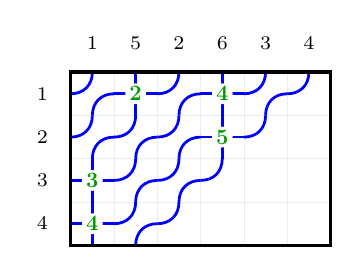
\begin{tikzpicture}[scale=0.55]
  \draw[lightgray, very thin, opacity=0.3] (0,2) -- (6,2);
  \draw[lightgray, very thin, opacity=0.3] (0,3) -- (6,3);
  \draw[lightgray, very thin, opacity=0.3] (0,4) -- (6,4);
  \draw[lightgray, very thin, opacity=0.3] (0,5) -- (6,5);
  \draw[lightgray, very thin, opacity=0.3] (0,6) -- (6,6);
  \draw[lightgray, very thin, opacity=0.3] (0,2) -- (0,6);
  \draw[lightgray, very thin, opacity=0.3] (1,2) -- (1,6);
  \draw[lightgray, very thin, opacity=0.3] (2,2) -- (2,6);
  \draw[lightgray, very thin, opacity=0.3] (3,2) -- (3,6);
  \draw[lightgray, very thin, opacity=0.3] (4,2) -- (4,6);
  \draw[lightgray, very thin, opacity=0.3] (5,2) -- (5,6);
  \draw[lightgray, very thin, opacity=0.3] (6,2) -- (6,6);
  \draw[blue, line width=1.0pt] (0,5.5) .. controls (0.3,5.5) and (0.5,5.7) .. (0.5,6);
  \draw[blue, line width=1.0pt] (0.5,5) .. controls (0.5,5.3) and (0.7,5.5) .. (1,5.5);
  \draw[blue, line width=1.0pt, line cap=round] (1,5.5) -- (2,5.5);
  \draw[blue, line width=1.0pt, line cap=round] (1.5,5) -- (1.5,6);
  \draw[blue, line width=1.0pt] (2,5.5) .. controls (2.3,5.5) and (2.5,5.7) .. (2.5,6);
  \draw[blue, line width=1.0pt] (2.5,5) .. controls (2.5,5.3) and (2.7,5.5) .. (3,5.5);
  \draw[blue, line width=1.0pt, line cap=round] (3,5.5) -- (4,5.5);
  \draw[blue, line width=1.0pt, line cap=round] (3.5,5) -- (3.5,6);
  \draw[blue, line width=1.0pt] (4,5.5) .. controls (4.3,5.5) and (4.5,5.7) .. (4.5,6);
  \draw[blue, line width=1.0pt] (4.5,5) .. controls (4.5,5.3) and (4.7,5.5) .. (5,5.5);
  \draw[blue, line width=1.0pt] (5,5.5) .. controls (5.3,5.5) and (5.5,5.7) .. (5.5,6);
  \draw[blue, line width=1.0pt] (0,4.5) .. controls (0.3,4.5) and (0.5,4.7) .. (0.5,5);
  \draw[blue, line width=1.0pt] (0.5,4) .. controls (0.5,4.3) and (0.7,4.5) .. (1,4.5);
  \draw[blue, line width=1.0pt] (1,4.5) .. controls (1.3,4.5) and (1.5,4.7) .. (1.5,5);
  \draw[blue, line width=1.0pt] (1.5,4) .. controls (1.5,4.3) and (1.7,4.5) .. (2,4.5);
  \draw[blue, line width=1.0pt] (2,4.5) .. controls (2.3,4.5) and (2.5,4.7) .. (2.5,5);
  \draw[blue, line width=1.0pt] (2.5,4) .. controls (2.5,4.3) and (2.7,4.5) .. (3,4.5);
  \draw[blue, line width=1.0pt, line cap=round] (3,4.5) -- (4,4.5);
  \draw[blue, line width=1.0pt, line cap=round] (3.5,4) -- (3.5,5);
  \draw[blue, line width=1.0pt] (4,4.5) .. controls (4.3,4.5) and (4.5,4.7) .. (4.5,5);
  \draw[blue, line width=1.0pt, line cap=round] (0,3.5) -- (1,3.5);
  \draw[blue, line width=1.0pt, line cap=round] (0.5,3) -- (0.5,4);
  \draw[blue, line width=1.0pt] (1,3.5) .. controls (1.3,3.5) and (1.5,3.7) .. (1.5,4);
  \draw[blue, line width=1.0pt] (1.5,3) .. controls (1.5,3.3) and (1.7,3.5) .. (2,3.5);
  \draw[blue, line width=1.0pt] (2,3.5) .. controls (2.3,3.5) and (2.5,3.7) .. (2.5,4);
  \draw[blue, line width=1.0pt] (2.5,3) .. controls (2.5,3.3) and (2.7,3.5) .. (3,3.5);
  \draw[blue, line width=1.0pt] (3,3.5) .. controls (3.3,3.5) and (3.5,3.7) .. (3.5,4);
  \draw[blue, line width=1.0pt, line cap=round] (0,2.5) -- (1,2.5);
  \draw[blue, line width=1.0pt, line cap=round] (0.5,2) -- (0.5,3);
  \draw[blue, line width=1.0pt] (1,2.5) .. controls (1.3,2.5) and (1.5,2.7) .. (1.5,3);
  \draw[blue, line width=1.0pt] (1.5,2) .. controls (1.5,2.3) and (1.7,2.5) .. (2,2.5);
  \draw[blue, line width=1.0pt] (2,2.5) .. controls (2.3,2.5) and (2.5,2.7) .. (2.5,3);
  \node[font=\Large\bfseries, text=green!60!black, fill=white, inner sep=0.5pt, circle, transform shape] at (3.5,4.5) {5};
  \node[font=\Large\bfseries, text=green!60!black, fill=white, inner sep=0.5pt, circle, transform shape] at (1.5,5.5) {2};
  \node[font=\Large\bfseries, text=green!60!black, fill=white, inner sep=0.5pt, circle, transform shape] at (0.5,3.5) {3};
  \node[font=\Large\bfseries, text=green!60!black, fill=white, inner sep=0.5pt, circle, transform shape] at (3.5,5.5) {4};
  \node[font=\Large\bfseries, text=green!60!black, fill=white, inner sep=0.5pt, circle, transform shape] at (0.5,2.5) {4};
  \node[font=\scriptsize, text=black, anchor=south] at (0.5,6.3) {1};
  \node[font=\scriptsize, text=black, anchor=south] at (1.5,6.3) {5};
  \node[font=\scriptsize, text=black, anchor=south] at (2.5,6.3) {2};
  \node[font=\scriptsize, text=black, anchor=south] at (3.5,6.3) {6};
  \node[font=\scriptsize, text=black, anchor=south] at (4.5,6.3) {3};
  \node[font=\scriptsize, text=black, anchor=south] at (5.5,6.3) {4};
  \node[font=\scriptsize, text=black, anchor=east] at (-0.3,5.5) {1};
  \node[font=\scriptsize, text=black, anchor=east] at (-0.3,4.5) {2};
  \node[font=\scriptsize, text=black, anchor=east] at (-0.3,3.5) {3};
  \node[font=\scriptsize, text=black, anchor=east] at (-0.3,2.5) {4};
  \draw[black, line width=1.2000000000000002pt] (0,2) rectangle (6,6);
\end{tikzpicture}}}
  +
  \vcenter{\hbox{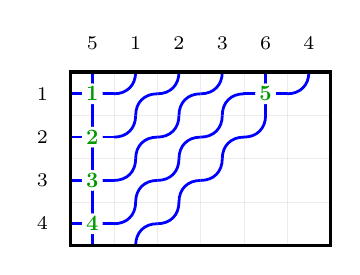
\begin{tikzpicture}[scale=0.55]
  \draw[lightgray, very thin, opacity=0.3] (0,2) -- (6,2);
  \draw[lightgray, very thin, opacity=0.3] (0,3) -- (6,3);
  \draw[lightgray, very thin, opacity=0.3] (0,4) -- (6,4);
  \draw[lightgray, very thin, opacity=0.3] (0,5) -- (6,5);
  \draw[lightgray, very thin, opacity=0.3] (0,6) -- (6,6);
  \draw[lightgray, very thin, opacity=0.3] (0,2) -- (0,6);
  \draw[lightgray, very thin, opacity=0.3] (1,2) -- (1,6);
  \draw[lightgray, very thin, opacity=0.3] (2,2) -- (2,6);
  \draw[lightgray, very thin, opacity=0.3] (3,2) -- (3,6);
  \draw[lightgray, very thin, opacity=0.3] (4,2) -- (4,6);
  \draw[lightgray, very thin, opacity=0.3] (5,2) -- (5,6);
  \draw[lightgray, very thin, opacity=0.3] (6,2) -- (6,6);
  \draw[blue, line width=1.0pt, line cap=round] (0,5.5) -- (1,5.5);
  \draw[blue, line width=1.0pt, line cap=round] (0.5,5) -- (0.5,6);
  \draw[blue, line width=1.0pt] (1,5.5) .. controls (1.3,5.5) and (1.5,5.7) .. (1.5,6);
  \draw[blue, line width=1.0pt] (1.5,5) .. controls (1.5,5.3) and (1.7,5.5) .. (2,5.5);
  \draw[blue, line width=1.0pt] (2,5.5) .. controls (2.3,5.5) and (2.5,5.7) .. (2.5,6);
  \draw[blue, line width=1.0pt] (2.5,5) .. controls (2.5,5.3) and (2.7,5.5) .. (3,5.5);
  \draw[blue, line width=1.0pt] (3,5.5) .. controls (3.3,5.5) and (3.5,5.7) .. (3.5,6);
  \draw[blue, line width=1.0pt] (3.5,5) .. controls (3.5,5.3) and (3.7,5.5) .. (4,5.5);
  \draw[blue, line width=1.0pt, line cap=round] (4,5.5) -- (5,5.5);
  \draw[blue, line width=1.0pt, line cap=round] (4.5,5) -- (4.5,6);
  \draw[blue, line width=1.0pt] (5,5.5) .. controls (5.3,5.5) and (5.5,5.7) .. (5.5,6);
  \draw[blue, line width=1.0pt, line cap=round] (0,4.5) -- (1,4.5);
  \draw[blue, line width=1.0pt, line cap=round] (0.5,4) -- (0.5,5);
  \draw[blue, line width=1.0pt] (1,4.5) .. controls (1.3,4.5) and (1.5,4.7) .. (1.5,5);
  \draw[blue, line width=1.0pt] (1.5,4) .. controls (1.5,4.3) and (1.7,4.5) .. (2,4.5);
  \draw[blue, line width=1.0pt] (2,4.5) .. controls (2.3,4.5) and (2.5,4.7) .. (2.5,5);
  \draw[blue, line width=1.0pt] (2.5,4) .. controls (2.5,4.3) and (2.7,4.5) .. (3,4.5);
  \draw[blue, line width=1.0pt] (3,4.5) .. controls (3.3,4.5) and (3.5,4.7) .. (3.5,5);
  \draw[blue, line width=1.0pt] (3.5,4) .. controls (3.5,4.3) and (3.7,4.5) .. (4,4.5);
  \draw[blue, line width=1.0pt] (4,4.5) .. controls (4.3,4.5) and (4.5,4.7) .. (4.5,5);
  \draw[blue, line width=1.0pt, line cap=round] (0,3.5) -- (1,3.5);
  \draw[blue, line width=1.0pt, line cap=round] (0.5,3) -- (0.5,4);
  \draw[blue, line width=1.0pt] (1,3.5) .. controls (1.3,3.5) and (1.5,3.7) .. (1.5,4);
  \draw[blue, line width=1.0pt] (1.5,3) .. controls (1.5,3.3) and (1.7,3.5) .. (2,3.5);
  \draw[blue, line width=1.0pt] (2,3.5) .. controls (2.3,3.5) and (2.5,3.7) .. (2.5,4);
  \draw[blue, line width=1.0pt] (2.5,3) .. controls (2.5,3.3) and (2.7,3.5) .. (3,3.5);
  \draw[blue, line width=1.0pt] (3,3.5) .. controls (3.3,3.5) and (3.5,3.7) .. (3.5,4);
  \draw[blue, line width=1.0pt, line cap=round] (0,2.5) -- (1,2.5);
  \draw[blue, line width=1.0pt, line cap=round] (0.5,2) -- (0.5,3);
  \draw[blue, line width=1.0pt] (1,2.5) .. controls (1.3,2.5) and (1.5,2.7) .. (1.5,3);
  \draw[blue, line width=1.0pt] (1.5,2) .. controls (1.5,2.3) and (1.7,2.5) .. (2,2.5);
  \draw[blue, line width=1.0pt] (2,2.5) .. controls (2.3,2.5) and (2.5,2.7) .. (2.5,3);
  \node[font=\Large\bfseries, text=green!60!black, fill=white, inner sep=0.5pt, circle, transform shape] at (0.5,4.5) {2};
  \node[font=\Large\bfseries, text=green!60!black, fill=white, inner sep=0.5pt, circle, transform shape] at (4.5,5.5) {5};
  \node[font=\Large\bfseries, text=green!60!black, fill=white, inner sep=0.5pt, circle, transform shape] at (0.5,3.5) {3};
  \node[font=\Large\bfseries, text=green!60!black, fill=white, inner sep=0.5pt, circle, transform shape] at (0.5,5.5) {1};
  \node[font=\Large\bfseries, text=green!60!black, fill=white, inner sep=0.5pt, circle, transform shape] at (0.5,2.5) {4};
  \node[font=\scriptsize, text=black, anchor=south] at (0.5,6.3) {5};
  \node[font=\scriptsize, text=black, anchor=south] at (1.5,6.3) {1};
  \node[font=\scriptsize, text=black, anchor=south] at (2.5,6.3) {2};
  \node[font=\scriptsize, text=black, anchor=south] at (3.5,6.3) {3};
  \node[font=\scriptsize, text=black, anchor=south] at (4.5,6.3) {6};
  \node[font=\scriptsize, text=black, anchor=south] at (5.5,6.3) {4};
  \node[font=\scriptsize, text=black, anchor=east] at (-0.3,5.5) {1};
  \node[font=\scriptsize, text=black, anchor=east] at (-0.3,4.5) {2};
  \node[font=\scriptsize, text=black, anchor=east] at (-0.3,3.5) {3};
  \node[font=\scriptsize, text=black, anchor=east] at (-0.3,2.5) {4};
  \draw[black, line width=1.2000000000000002pt] (0,2) rectangle (6,6);
\end{tikzpicture}}}
  \\[1em]
  + & 
  \vcenter{\hbox{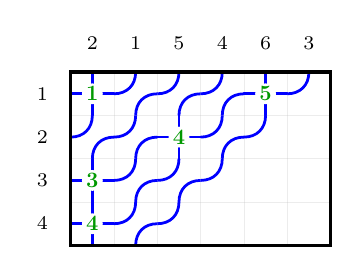
\begin{tikzpicture}[scale=0.55]
  \draw[lightgray, very thin, opacity=0.3] (0,2) -- (6,2);
  \draw[lightgray, very thin, opacity=0.3] (0,3) -- (6,3);
  \draw[lightgray, very thin, opacity=0.3] (0,4) -- (6,4);
  \draw[lightgray, very thin, opacity=0.3] (0,5) -- (6,5);
  \draw[lightgray, very thin, opacity=0.3] (0,6) -- (6,6);
  \draw[lightgray, very thin, opacity=0.3] (0,2) -- (0,6);
  \draw[lightgray, very thin, opacity=0.3] (1,2) -- (1,6);
  \draw[lightgray, very thin, opacity=0.3] (2,2) -- (2,6);
  \draw[lightgray, very thin, opacity=0.3] (3,2) -- (3,6);
  \draw[lightgray, very thin, opacity=0.3] (4,2) -- (4,6);
  \draw[lightgray, very thin, opacity=0.3] (5,2) -- (5,6);
  \draw[lightgray, very thin, opacity=0.3] (6,2) -- (6,6);
  \draw[blue, line width=1.0pt, line cap=round] (0,5.5) -- (1,5.5);
  \draw[blue, line width=1.0pt, line cap=round] (0.5,5) -- (0.5,6);
  \draw[blue, line width=1.0pt] (1,5.5) .. controls (1.3,5.5) and (1.5,5.7) .. (1.5,6);
  \draw[blue, line width=1.0pt] (1.5,5) .. controls (1.5,5.3) and (1.7,5.5) .. (2,5.5);
  \draw[blue, line width=1.0pt] (2,5.5) .. controls (2.3,5.5) and (2.5,5.7) .. (2.5,6);
  \draw[blue, line width=1.0pt] (2.5,5) .. controls (2.5,5.3) and (2.7,5.5) .. (3,5.5);
  \draw[blue, line width=1.0pt] (3,5.5) .. controls (3.3,5.5) and (3.5,5.7) .. (3.5,6);
  \draw[blue, line width=1.0pt] (3.5,5) .. controls (3.5,5.3) and (3.7,5.5) .. (4,5.5);
  \draw[blue, line width=1.0pt, line cap=round] (4,5.5) -- (5,5.5);
  \draw[blue, line width=1.0pt, line cap=round] (4.5,5) -- (4.5,6);
  \draw[blue, line width=1.0pt] (5,5.5) .. controls (5.3,5.5) and (5.5,5.7) .. (5.5,6);
  \draw[blue, line width=1.0pt] (0,4.5) .. controls (0.3,4.5) and (0.5,4.7) .. (0.5,5);
  \draw[blue, line width=1.0pt] (0.5,4) .. controls (0.5,4.3) and (0.7,4.5) .. (1,4.5);
  \draw[blue, line width=1.0pt] (1,4.5) .. controls (1.3,4.5) and (1.5,4.7) .. (1.5,5);
  \draw[blue, line width=1.0pt] (1.5,4) .. controls (1.5,4.3) and (1.7,4.5) .. (2,4.5);
  \draw[blue, line width=1.0pt, line cap=round] (2,4.5) -- (3,4.5);
  \draw[blue, line width=1.0pt, line cap=round] (2.5,4) -- (2.5,5);
  \draw[blue, line width=1.0pt] (3,4.5) .. controls (3.3,4.5) and (3.5,4.7) .. (3.5,5);
  \draw[blue, line width=1.0pt] (3.5,4) .. controls (3.5,4.3) and (3.7,4.5) .. (4,4.5);
  \draw[blue, line width=1.0pt] (4,4.5) .. controls (4.3,4.5) and (4.5,4.7) .. (4.5,5);
  \draw[blue, line width=1.0pt, line cap=round] (0,3.5) -- (1,3.5);
  \draw[blue, line width=1.0pt, line cap=round] (0.5,3) -- (0.5,4);
  \draw[blue, line width=1.0pt] (1,3.5) .. controls (1.3,3.5) and (1.5,3.7) .. (1.5,4);
  \draw[blue, line width=1.0pt] (1.5,3) .. controls (1.5,3.3) and (1.7,3.5) .. (2,3.5);
  \draw[blue, line width=1.0pt] (2,3.5) .. controls (2.3,3.5) and (2.5,3.7) .. (2.5,4);
  \draw[blue, line width=1.0pt] (2.5,3) .. controls (2.5,3.3) and (2.7,3.5) .. (3,3.5);
  \draw[blue, line width=1.0pt] (3,3.5) .. controls (3.3,3.5) and (3.5,3.7) .. (3.5,4);
  \draw[blue, line width=1.0pt, line cap=round] (0,2.5) -- (1,2.5);
  \draw[blue, line width=1.0pt, line cap=round] (0.5,2) -- (0.5,3);
  \draw[blue, line width=1.0pt] (1,2.5) .. controls (1.3,2.5) and (1.5,2.7) .. (1.5,3);
  \draw[blue, line width=1.0pt] (1.5,2) .. controls (1.5,2.3) and (1.7,2.5) .. (2,2.5);
  \draw[blue, line width=1.0pt] (2,2.5) .. controls (2.3,2.5) and (2.5,2.7) .. (2.5,3);
  \node[font=\Large\bfseries, text=green!60!black, fill=white, inner sep=0.5pt, circle, transform shape] at (4.5,5.5) {5};
  \node[font=\Large\bfseries, text=green!60!black, fill=white, inner sep=0.5pt, circle, transform shape] at (0.5,3.5) {3};
  \node[font=\Large\bfseries, text=green!60!black, fill=white, inner sep=0.5pt, circle, transform shape] at (0.5,5.5) {1};
  \node[font=\Large\bfseries, text=green!60!black, fill=white, inner sep=0.5pt, circle, transform shape] at (2.5,4.5) {4};
  \node[font=\Large\bfseries, text=green!60!black, fill=white, inner sep=0.5pt, circle, transform shape] at (0.5,2.5) {4};
  \node[font=\scriptsize, text=black, anchor=south] at (0.5,6.3) {2};
  \node[font=\scriptsize, text=black, anchor=south] at (1.5,6.3) {1};
  \node[font=\scriptsize, text=black, anchor=south] at (2.5,6.3) {5};
  \node[font=\scriptsize, text=black, anchor=south] at (3.5,6.3) {4};
  \node[font=\scriptsize, text=black, anchor=south] at (4.5,6.3) {6};
  \node[font=\scriptsize, text=black, anchor=south] at (5.5,6.3) {3};
  \node[font=\scriptsize, text=black, anchor=east] at (-0.3,5.5) {1};
  \node[font=\scriptsize, text=black, anchor=east] at (-0.3,4.5) {2};
  \node[font=\scriptsize, text=black, anchor=east] at (-0.3,3.5) {3};
  \node[font=\scriptsize, text=black, anchor=east] at (-0.3,2.5) {4};
  \draw[black, line width=1.2000000000000002pt] (0,2) rectangle (6,6);
\end{tikzpicture}}}
  +
  \vcenter{\hbox{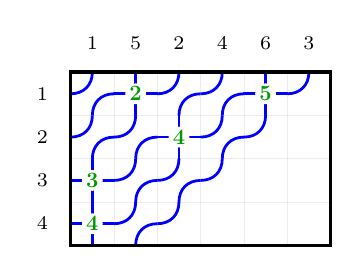
\begin{tikzpicture}[scale=0.55]
  \draw[lightgray, very thin, opacity=0.3] (0,2) -- (6,2);
  \draw[lightgray, very thin, opacity=0.3] (0,3) -- (6,3);
  \draw[lightgray, very thin, opacity=0.3] (0,4) -- (6,4);
  \draw[lightgray, very thin, opacity=0.3] (0,5) -- (6,5);
  \draw[lightgray, very thin, opacity=0.3] (0,6) -- (6,6);
  \draw[lightgray, very thin, opacity=0.3] (0,2) -- (0,6);
  \draw[lightgray, very thin, opacity=0.3] (1,2) -- (1,6);
  \draw[lightgray, very thin, opacity=0.3] (2,2) -- (2,6);
  \draw[lightgray, very thin, opacity=0.3] (3,2) -- (3,6);
  \draw[lightgray, very thin, opacity=0.3] (4,2) -- (4,6);
  \draw[lightgray, very thin, opacity=0.3] (5,2) -- (5,6);
  \draw[lightgray, very thin, opacity=0.3] (6,2) -- (6,6);
  \draw[blue, line width=1.0pt] (0,5.5) .. controls (0.3,5.5) and (0.5,5.7) .. (0.5,6);
  \draw[blue, line width=1.0pt] (0.5,5) .. controls (0.5,5.3) and (0.7,5.5) .. (1,5.5);
  \draw[blue, line width=1.0pt, line cap=round] (1,5.5) -- (2,5.5);
  \draw[blue, line width=1.0pt, line cap=round] (1.5,5) -- (1.5,6);
  \draw[blue, line width=1.0pt] (2,5.5) .. controls (2.3,5.5) and (2.5,5.7) .. (2.5,6);
  \draw[blue, line width=1.0pt] (2.5,5) .. controls (2.5,5.3) and (2.7,5.5) .. (3,5.5);
  \draw[blue, line width=1.0pt] (3,5.5) .. controls (3.3,5.5) and (3.5,5.7) .. (3.5,6);
  \draw[blue, line width=1.0pt] (3.5,5) .. controls (3.5,5.3) and (3.7,5.5) .. (4,5.5);
  \draw[blue, line width=1.0pt, line cap=round] (4,5.5) -- (5,5.5);
  \draw[blue, line width=1.0pt, line cap=round] (4.5,5) -- (4.5,6);
  \draw[blue, line width=1.0pt] (5,5.5) .. controls (5.3,5.5) and (5.5,5.7) .. (5.5,6);
  \draw[blue, line width=1.0pt] (0,4.5) .. controls (0.3,4.5) and (0.5,4.7) .. (0.5,5);
  \draw[blue, line width=1.0pt] (0.5,4) .. controls (0.5,4.3) and (0.7,4.5) .. (1,4.5);
  \draw[blue, line width=1.0pt] (1,4.5) .. controls (1.3,4.5) and (1.5,4.7) .. (1.5,5);
  \draw[blue, line width=1.0pt] (1.5,4) .. controls (1.5,4.3) and (1.7,4.5) .. (2,4.5);
  \draw[blue, line width=1.0pt, line cap=round] (2,4.5) -- (3,4.5);
  \draw[blue, line width=1.0pt, line cap=round] (2.5,4) -- (2.5,5);
  \draw[blue, line width=1.0pt] (3,4.5) .. controls (3.3,4.5) and (3.5,4.7) .. (3.5,5);
  \draw[blue, line width=1.0pt] (3.5,4) .. controls (3.5,4.3) and (3.7,4.5) .. (4,4.5);
  \draw[blue, line width=1.0pt] (4,4.5) .. controls (4.3,4.5) and (4.5,4.7) .. (4.5,5);
  \draw[blue, line width=1.0pt, line cap=round] (0,3.5) -- (1,3.5);
  \draw[blue, line width=1.0pt, line cap=round] (0.5,3) -- (0.5,4);
  \draw[blue, line width=1.0pt] (1,3.5) .. controls (1.3,3.5) and (1.5,3.7) .. (1.5,4);
  \draw[blue, line width=1.0pt] (1.5,3) .. controls (1.5,3.3) and (1.7,3.5) .. (2,3.5);
  \draw[blue, line width=1.0pt] (2,3.5) .. controls (2.3,3.5) and (2.5,3.7) .. (2.5,4);
  \draw[blue, line width=1.0pt] (2.5,3) .. controls (2.5,3.3) and (2.7,3.5) .. (3,3.5);
  \draw[blue, line width=1.0pt] (3,3.5) .. controls (3.3,3.5) and (3.5,3.7) .. (3.5,4);
  \draw[blue, line width=1.0pt, line cap=round] (0,2.5) -- (1,2.5);
  \draw[blue, line width=1.0pt, line cap=round] (0.5,2) -- (0.5,3);
  \draw[blue, line width=1.0pt] (1,2.5) .. controls (1.3,2.5) and (1.5,2.7) .. (1.5,3);
  \draw[blue, line width=1.0pt] (1.5,2) .. controls (1.5,2.3) and (1.7,2.5) .. (2,2.5);
  \draw[blue, line width=1.0pt] (2,2.5) .. controls (2.3,2.5) and (2.5,2.7) .. (2.5,3);
  \node[font=\Large\bfseries, text=green!60!black, fill=white, inner sep=0.5pt, circle, transform shape] at (1.5,5.5) {2};
  \node[font=\Large\bfseries, text=green!60!black, fill=white, inner sep=0.5pt, circle, transform shape] at (4.5,5.5) {5};
  \node[font=\Large\bfseries, text=green!60!black, fill=white, inner sep=0.5pt, circle, transform shape] at (0.5,3.5) {3};
  \node[font=\Large\bfseries, text=green!60!black, fill=white, inner sep=0.5pt, circle, transform shape] at (2.5,4.5) {4};
  \node[font=\Large\bfseries, text=green!60!black, fill=white, inner sep=0.5pt, circle, transform shape] at (0.5,2.5) {4};
  \node[font=\scriptsize, text=black, anchor=south] at (0.5,6.3) {1};
  \node[font=\scriptsize, text=black, anchor=south] at (1.5,6.3) {5};
  \node[font=\scriptsize, text=black, anchor=south] at (2.5,6.3) {2};
  \node[font=\scriptsize, text=black, anchor=south] at (3.5,6.3) {4};
  \node[font=\scriptsize, text=black, anchor=south] at (4.5,6.3) {6};
  \node[font=\scriptsize, text=black, anchor=south] at (5.5,6.3) {3};
  \node[font=\scriptsize, text=black, anchor=east] at (-0.3,5.5) {1};
  \node[font=\scriptsize, text=black, anchor=east] at (-0.3,4.5) {2};
  \node[font=\scriptsize, text=black, anchor=east] at (-0.3,3.5) {3};
  \node[font=\scriptsize, text=black, anchor=east] at (-0.3,2.5) {4};
  \draw[black, line width=1.2000000000000002pt] (0,2) rectangle (6,6);
\end{tikzpicture}}}
  +
  \vcenter{\hbox{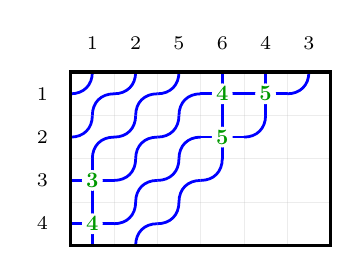
\begin{tikzpicture}[scale=0.55]
  \draw[lightgray, very thin, opacity=0.3] (0,2) -- (6,2);
  \draw[lightgray, very thin, opacity=0.3] (0,3) -- (6,3);
  \draw[lightgray, very thin, opacity=0.3] (0,4) -- (6,4);
  \draw[lightgray, very thin, opacity=0.3] (0,5) -- (6,5);
  \draw[lightgray, very thin, opacity=0.3] (0,6) -- (6,6);
  \draw[lightgray, very thin, opacity=0.3] (0,2) -- (0,6);
  \draw[lightgray, very thin, opacity=0.3] (1,2) -- (1,6);
  \draw[lightgray, very thin, opacity=0.3] (2,2) -- (2,6);
  \draw[lightgray, very thin, opacity=0.3] (3,2) -- (3,6);
  \draw[lightgray, very thin, opacity=0.3] (4,2) -- (4,6);
  \draw[lightgray, very thin, opacity=0.3] (5,2) -- (5,6);
  \draw[lightgray, very thin, opacity=0.3] (6,2) -- (6,6);
  \draw[blue, line width=1.0pt] (0,5.5) .. controls (0.3,5.5) and (0.5,5.7) .. (0.5,6);
  \draw[blue, line width=1.0pt] (0.5,5) .. controls (0.5,5.3) and (0.7,5.5) .. (1,5.5);
  \draw[blue, line width=1.0pt] (1,5.5) .. controls (1.3,5.5) and (1.5,5.7) .. (1.5,6);
  \draw[blue, line width=1.0pt] (1.5,5) .. controls (1.5,5.3) and (1.7,5.5) .. (2,5.5);
  \draw[blue, line width=1.0pt] (2,5.5) .. controls (2.3,5.5) and (2.5,5.7) .. (2.5,6);
  \draw[blue, line width=1.0pt] (2.5,5) .. controls (2.5,5.3) and (2.7,5.5) .. (3,5.5);
  \draw[blue, line width=1.0pt, line cap=round] (3,5.5) -- (4,5.5);
  \draw[blue, line width=1.0pt, line cap=round] (3.5,5) -- (3.5,6);
  \draw[blue, line width=1.0pt, line cap=round] (4,5.5) -- (5,5.5);
  \draw[blue, line width=1.0pt, line cap=round] (4.5,5) -- (4.5,6);
  \draw[blue, line width=1.0pt] (5,5.5) .. controls (5.3,5.5) and (5.5,5.7) .. (5.5,6);
  \draw[blue, line width=1.0pt] (0,4.5) .. controls (0.3,4.5) and (0.5,4.7) .. (0.5,5);
  \draw[blue, line width=1.0pt] (0.5,4) .. controls (0.5,4.3) and (0.7,4.5) .. (1,4.5);
  \draw[blue, line width=1.0pt] (1,4.5) .. controls (1.3,4.5) and (1.5,4.7) .. (1.5,5);
  \draw[blue, line width=1.0pt] (1.5,4) .. controls (1.5,4.3) and (1.7,4.5) .. (2,4.5);
  \draw[blue, line width=1.0pt] (2,4.5) .. controls (2.3,4.5) and (2.5,4.7) .. (2.5,5);
  \draw[blue, line width=1.0pt] (2.5,4) .. controls (2.5,4.3) and (2.7,4.5) .. (3,4.5);
  \draw[blue, line width=1.0pt, line cap=round] (3,4.5) -- (4,4.5);
  \draw[blue, line width=1.0pt, line cap=round] (3.5,4) -- (3.5,5);
  \draw[blue, line width=1.0pt] (4,4.5) .. controls (4.3,4.5) and (4.5,4.7) .. (4.5,5);
  \draw[blue, line width=1.0pt, line cap=round] (0,3.5) -- (1,3.5);
  \draw[blue, line width=1.0pt, line cap=round] (0.5,3) -- (0.5,4);
  \draw[blue, line width=1.0pt] (1,3.5) .. controls (1.3,3.5) and (1.5,3.7) .. (1.5,4);
  \draw[blue, line width=1.0pt] (1.5,3) .. controls (1.5,3.3) and (1.7,3.5) .. (2,3.5);
  \draw[blue, line width=1.0pt] (2,3.5) .. controls (2.3,3.5) and (2.5,3.7) .. (2.5,4);
  \draw[blue, line width=1.0pt] (2.5,3) .. controls (2.5,3.3) and (2.7,3.5) .. (3,3.5);
  \draw[blue, line width=1.0pt] (3,3.5) .. controls (3.3,3.5) and (3.5,3.7) .. (3.5,4);
  \draw[blue, line width=1.0pt, line cap=round] (0,2.5) -- (1,2.5);
  \draw[blue, line width=1.0pt, line cap=round] (0.5,2) -- (0.5,3);
  \draw[blue, line width=1.0pt] (1,2.5) .. controls (1.3,2.5) and (1.5,2.7) .. (1.5,3);
  \draw[blue, line width=1.0pt] (1.5,2) .. controls (1.5,2.3) and (1.7,2.5) .. (2,2.5);
  \draw[blue, line width=1.0pt] (2,2.5) .. controls (2.3,2.5) and (2.5,2.7) .. (2.5,3);
  \node[font=\Large\bfseries, text=green!60!black, fill=white, inner sep=0.5pt, circle, transform shape] at (3.5,4.5) {5};
  \node[font=\Large\bfseries, text=green!60!black, fill=white, inner sep=0.5pt, circle, transform shape] at (4.5,5.5) {5};
  \node[font=\Large\bfseries, text=green!60!black, fill=white, inner sep=0.5pt, circle, transform shape] at (0.5,3.5) {3};
  \node[font=\Large\bfseries, text=green!60!black, fill=white, inner sep=0.5pt, circle, transform shape] at (3.5,5.5) {4};
  \node[font=\Large\bfseries, text=green!60!black, fill=white, inner sep=0.5pt, circle, transform shape] at (0.5,2.5) {4};
  \node[font=\scriptsize, text=black, anchor=south] at (0.5,6.3) {1};
  \node[font=\scriptsize, text=black, anchor=south] at (1.5,6.3) {2};
  \node[font=\scriptsize, text=black, anchor=south] at (2.5,6.3) {5};
  \node[font=\scriptsize, text=black, anchor=south] at (3.5,6.3) {6};
  \node[font=\scriptsize, text=black, anchor=south] at (4.5,6.3) {4};
  \node[font=\scriptsize, text=black, anchor=south] at (5.5,6.3) {3};
  \node[font=\scriptsize, text=black, anchor=east] at (-0.3,5.5) {1};
  \node[font=\scriptsize, text=black, anchor=east] at (-0.3,4.5) {2};
  \node[font=\scriptsize, text=black, anchor=east] at (-0.3,3.5) {3};
  \node[font=\scriptsize, text=black, anchor=east] at (-0.3,2.5) {4};
  \draw[black, line width=1.2000000000000002pt] (0,2) rectangle (6,6);
\end{tikzpicture}}}
  \\[1em]
  + & 
  \vcenter{\hbox{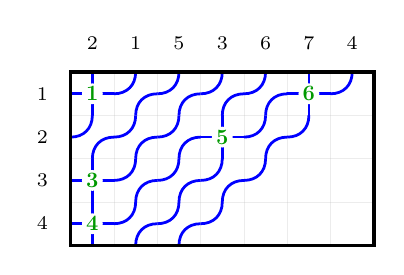
\begin{tikzpicture}[scale=0.55]
  \draw[lightgray, very thin, opacity=0.3] (0,3) -- (7,3);
  \draw[lightgray, very thin, opacity=0.3] (0,4) -- (7,4);
  \draw[lightgray, very thin, opacity=0.3] (0,5) -- (7,5);
  \draw[lightgray, very thin, opacity=0.3] (0,6) -- (7,6);
  \draw[lightgray, very thin, opacity=0.3] (0,7) -- (7,7);
  \draw[lightgray, very thin, opacity=0.3] (0,3) -- (0,7);
  \draw[lightgray, very thin, opacity=0.3] (1,3) -- (1,7);
  \draw[lightgray, very thin, opacity=0.3] (2,3) -- (2,7);
  \draw[lightgray, very thin, opacity=0.3] (3,3) -- (3,7);
  \draw[lightgray, very thin, opacity=0.3] (4,3) -- (4,7);
  \draw[lightgray, very thin, opacity=0.3] (5,3) -- (5,7);
  \draw[lightgray, very thin, opacity=0.3] (6,3) -- (6,7);
  \draw[lightgray, very thin, opacity=0.3] (7,3) -- (7,7);
  \draw[blue, line width=1.0pt, line cap=round] (0,6.5) -- (1,6.5);
  \draw[blue, line width=1.0pt, line cap=round] (0.5,6) -- (0.5,7);
  \draw[blue, line width=1.0pt] (1,6.5) .. controls (1.3,6.5) and (1.5,6.7) .. (1.5,7);
  \draw[blue, line width=1.0pt] (1.5,6) .. controls (1.5,6.3) and (1.7,6.5) .. (2,6.5);
  \draw[blue, line width=1.0pt] (2,6.5) .. controls (2.3,6.5) and (2.5,6.7) .. (2.5,7);
  \draw[blue, line width=1.0pt] (2.5,6) .. controls (2.5,6.3) and (2.7,6.5) .. (3,6.5);
  \draw[blue, line width=1.0pt] (3,6.5) .. controls (3.3,6.5) and (3.5,6.7) .. (3.5,7);
  \draw[blue, line width=1.0pt] (3.5,6) .. controls (3.5,6.3) and (3.7,6.5) .. (4,6.5);
  \draw[blue, line width=1.0pt] (4,6.5) .. controls (4.3,6.5) and (4.5,6.7) .. (4.5,7);
  \draw[blue, line width=1.0pt] (4.5,6) .. controls (4.5,6.3) and (4.7,6.5) .. (5,6.5);
  \draw[blue, line width=1.0pt, line cap=round] (5,6.5) -- (6,6.5);
  \draw[blue, line width=1.0pt, line cap=round] (5.5,6) -- (5.5,7);
  \draw[blue, line width=1.0pt] (6,6.5) .. controls (6.3,6.5) and (6.5,6.7) .. (6.5,7);
  \draw[blue, line width=1.0pt] (0,5.5) .. controls (0.3,5.5) and (0.5,5.7) .. (0.5,6);
  \draw[blue, line width=1.0pt] (0.5,5) .. controls (0.5,5.3) and (0.7,5.5) .. (1,5.5);
  \draw[blue, line width=1.0pt] (1,5.5) .. controls (1.3,5.5) and (1.5,5.7) .. (1.5,6);
  \draw[blue, line width=1.0pt] (1.5,5) .. controls (1.5,5.3) and (1.7,5.5) .. (2,5.5);
  \draw[blue, line width=1.0pt] (2,5.5) .. controls (2.3,5.5) and (2.5,5.7) .. (2.5,6);
  \draw[blue, line width=1.0pt] (2.5,5) .. controls (2.5,5.3) and (2.7,5.5) .. (3,5.5);
  \draw[blue, line width=1.0pt, line cap=round] (3,5.5) -- (4,5.5);
  \draw[blue, line width=1.0pt, line cap=round] (3.5,5) -- (3.5,6);
  \draw[blue, line width=1.0pt] (4,5.5) .. controls (4.3,5.5) and (4.5,5.7) .. (4.5,6);
  \draw[blue, line width=1.0pt] (4.5,5) .. controls (4.5,5.3) and (4.7,5.5) .. (5,5.5);
  \draw[blue, line width=1.0pt] (5,5.5) .. controls (5.3,5.5) and (5.5,5.7) .. (5.5,6);
  \draw[blue, line width=1.0pt, line cap=round] (0,4.5) -- (1,4.5);
  \draw[blue, line width=1.0pt, line cap=round] (0.5,4) -- (0.5,5);
  \draw[blue, line width=1.0pt] (1,4.5) .. controls (1.3,4.5) and (1.5,4.7) .. (1.5,5);
  \draw[blue, line width=1.0pt] (1.5,4) .. controls (1.5,4.3) and (1.7,4.5) .. (2,4.5);
  \draw[blue, line width=1.0pt] (2,4.5) .. controls (2.3,4.5) and (2.5,4.7) .. (2.5,5);
  \draw[blue, line width=1.0pt] (2.5,4) .. controls (2.5,4.3) and (2.7,4.5) .. (3,4.5);
  \draw[blue, line width=1.0pt] (3,4.5) .. controls (3.3,4.5) and (3.5,4.7) .. (3.5,5);
  \draw[blue, line width=1.0pt] (3.5,4) .. controls (3.5,4.3) and (3.7,4.5) .. (4,4.5);
  \draw[blue, line width=1.0pt] (4,4.5) .. controls (4.3,4.5) and (4.5,4.7) .. (4.5,5);
  \draw[blue, line width=1.0pt, line cap=round] (0,3.5) -- (1,3.5);
  \draw[blue, line width=1.0pt, line cap=round] (0.5,3) -- (0.5,4);
  \draw[blue, line width=1.0pt] (1,3.5) .. controls (1.3,3.5) and (1.5,3.7) .. (1.5,4);
  \draw[blue, line width=1.0pt] (1.5,3) .. controls (1.5,3.3) and (1.7,3.5) .. (2,3.5);
  \draw[blue, line width=1.0pt] (2,3.5) .. controls (2.3,3.5) and (2.5,3.7) .. (2.5,4);
  \draw[blue, line width=1.0pt] (2.5,3) .. controls (2.5,3.3) and (2.7,3.5) .. (3,3.5);
  \draw[blue, line width=1.0pt] (3,3.5) .. controls (3.3,3.5) and (3.5,3.7) .. (3.5,4);
  \node[font=\Large\bfseries, text=green!60!black, fill=white, inner sep=0.5pt, circle, transform shape] at (3.5,5.5) {5};
  \node[font=\Large\bfseries, text=green!60!black, fill=white, inner sep=0.5pt, circle, transform shape] at (0.5,4.5) {3};
  \node[font=\Large\bfseries, text=green!60!black, fill=white, inner sep=0.5pt, circle, transform shape] at (0.5,6.5) {1};
  \node[font=\Large\bfseries, text=green!60!black, fill=white, inner sep=0.5pt, circle, transform shape] at (5.5,6.5) {6};
  \node[font=\Large\bfseries, text=green!60!black, fill=white, inner sep=0.5pt, circle, transform shape] at (0.5,3.5) {4};
  \node[font=\scriptsize, text=black, anchor=south] at (0.5,7.3) {2};
  \node[font=\scriptsize, text=black, anchor=south] at (1.5,7.3) {1};
  \node[font=\scriptsize, text=black, anchor=south] at (2.5,7.3) {5};
  \node[font=\scriptsize, text=black, anchor=south] at (3.5,7.3) {3};
  \node[font=\scriptsize, text=black, anchor=south] at (4.5,7.3) {6};
  \node[font=\scriptsize, text=black, anchor=south] at (5.5,7.3) {7};
  \node[font=\scriptsize, text=black, anchor=south] at (6.5,7.3) {4};
  \node[font=\scriptsize, text=black, anchor=east] at (-0.3,6.5) {1};
  \node[font=\scriptsize, text=black, anchor=east] at (-0.3,5.5) {2};
  \node[font=\scriptsize, text=black, anchor=east] at (-0.3,4.5) {3};
  \node[font=\scriptsize, text=black, anchor=east] at (-0.3,3.5) {4};
  \draw[black, line width=1.2000000000000002pt] (0,3) rectangle (7,7);
\end{tikzpicture}}}
  +
  \vcenter{\hbox{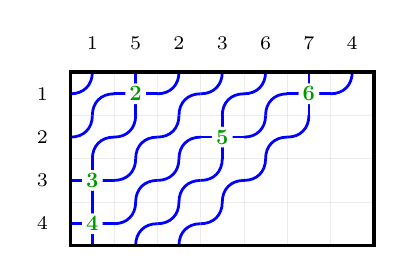
\begin{tikzpicture}[scale=0.55]
  \draw[lightgray, very thin, opacity=0.3] (0,3) -- (7,3);
  \draw[lightgray, very thin, opacity=0.3] (0,4) -- (7,4);
  \draw[lightgray, very thin, opacity=0.3] (0,5) -- (7,5);
  \draw[lightgray, very thin, opacity=0.3] (0,6) -- (7,6);
  \draw[lightgray, very thin, opacity=0.3] (0,7) -- (7,7);
  \draw[lightgray, very thin, opacity=0.3] (0,3) -- (0,7);
  \draw[lightgray, very thin, opacity=0.3] (1,3) -- (1,7);
  \draw[lightgray, very thin, opacity=0.3] (2,3) -- (2,7);
  \draw[lightgray, very thin, opacity=0.3] (3,3) -- (3,7);
  \draw[lightgray, very thin, opacity=0.3] (4,3) -- (4,7);
  \draw[lightgray, very thin, opacity=0.3] (5,3) -- (5,7);
  \draw[lightgray, very thin, opacity=0.3] (6,3) -- (6,7);
  \draw[lightgray, very thin, opacity=0.3] (7,3) -- (7,7);
  \draw[blue, line width=1.0pt] (0,6.5) .. controls (0.3,6.5) and (0.5,6.7) .. (0.5,7);
  \draw[blue, line width=1.0pt] (0.5,6) .. controls (0.5,6.3) and (0.7,6.5) .. (1,6.5);
  \draw[blue, line width=1.0pt, line cap=round] (1,6.5) -- (2,6.5);
  \draw[blue, line width=1.0pt, line cap=round] (1.5,6) -- (1.5,7);
  \draw[blue, line width=1.0pt] (2,6.5) .. controls (2.3,6.5) and (2.5,6.7) .. (2.5,7);
  \draw[blue, line width=1.0pt] (2.5,6) .. controls (2.5,6.3) and (2.7,6.5) .. (3,6.5);
  \draw[blue, line width=1.0pt] (3,6.5) .. controls (3.3,6.5) and (3.5,6.7) .. (3.5,7);
  \draw[blue, line width=1.0pt] (3.5,6) .. controls (3.5,6.3) and (3.7,6.5) .. (4,6.5);
  \draw[blue, line width=1.0pt] (4,6.5) .. controls (4.3,6.5) and (4.5,6.7) .. (4.5,7);
  \draw[blue, line width=1.0pt] (4.5,6) .. controls (4.5,6.3) and (4.7,6.5) .. (5,6.5);
  \draw[blue, line width=1.0pt, line cap=round] (5,6.5) -- (6,6.5);
  \draw[blue, line width=1.0pt, line cap=round] (5.5,6) -- (5.5,7);
  \draw[blue, line width=1.0pt] (6,6.5) .. controls (6.3,6.5) and (6.5,6.7) .. (6.5,7);
  \draw[blue, line width=1.0pt] (0,5.5) .. controls (0.3,5.5) and (0.5,5.7) .. (0.5,6);
  \draw[blue, line width=1.0pt] (0.5,5) .. controls (0.5,5.3) and (0.7,5.5) .. (1,5.5);
  \draw[blue, line width=1.0pt] (1,5.5) .. controls (1.3,5.5) and (1.5,5.7) .. (1.5,6);
  \draw[blue, line width=1.0pt] (1.5,5) .. controls (1.5,5.3) and (1.7,5.5) .. (2,5.5);
  \draw[blue, line width=1.0pt] (2,5.5) .. controls (2.3,5.5) and (2.5,5.7) .. (2.5,6);
  \draw[blue, line width=1.0pt] (2.5,5) .. controls (2.5,5.3) and (2.7,5.5) .. (3,5.5);
  \draw[blue, line width=1.0pt, line cap=round] (3,5.5) -- (4,5.5);
  \draw[blue, line width=1.0pt, line cap=round] (3.5,5) -- (3.5,6);
  \draw[blue, line width=1.0pt] (4,5.5) .. controls (4.3,5.5) and (4.5,5.7) .. (4.5,6);
  \draw[blue, line width=1.0pt] (4.5,5) .. controls (4.5,5.3) and (4.7,5.5) .. (5,5.5);
  \draw[blue, line width=1.0pt] (5,5.5) .. controls (5.3,5.5) and (5.5,5.7) .. (5.5,6);
  \draw[blue, line width=1.0pt, line cap=round] (0,4.5) -- (1,4.5);
  \draw[blue, line width=1.0pt, line cap=round] (0.5,4) -- (0.5,5);
  \draw[blue, line width=1.0pt] (1,4.5) .. controls (1.3,4.5) and (1.5,4.7) .. (1.5,5);
  \draw[blue, line width=1.0pt] (1.5,4) .. controls (1.5,4.3) and (1.7,4.5) .. (2,4.5);
  \draw[blue, line width=1.0pt] (2,4.5) .. controls (2.3,4.5) and (2.5,4.7) .. (2.5,5);
  \draw[blue, line width=1.0pt] (2.5,4) .. controls (2.5,4.3) and (2.7,4.5) .. (3,4.5);
  \draw[blue, line width=1.0pt] (3,4.5) .. controls (3.3,4.5) and (3.5,4.7) .. (3.5,5);
  \draw[blue, line width=1.0pt] (3.5,4) .. controls (3.5,4.3) and (3.7,4.5) .. (4,4.5);
  \draw[blue, line width=1.0pt] (4,4.5) .. controls (4.3,4.5) and (4.5,4.7) .. (4.5,5);
  \draw[blue, line width=1.0pt, line cap=round] (0,3.5) -- (1,3.5);
  \draw[blue, line width=1.0pt, line cap=round] (0.5,3) -- (0.5,4);
  \draw[blue, line width=1.0pt] (1,3.5) .. controls (1.3,3.5) and (1.5,3.7) .. (1.5,4);
  \draw[blue, line width=1.0pt] (1.5,3) .. controls (1.5,3.3) and (1.7,3.5) .. (2,3.5);
  \draw[blue, line width=1.0pt] (2,3.5) .. controls (2.3,3.5) and (2.5,3.7) .. (2.5,4);
  \draw[blue, line width=1.0pt] (2.5,3) .. controls (2.5,3.3) and (2.7,3.5) .. (3,3.5);
  \draw[blue, line width=1.0pt] (3,3.5) .. controls (3.3,3.5) and (3.5,3.7) .. (3.5,4);
  \node[font=\Large\bfseries, text=green!60!black, fill=white, inner sep=0.5pt, circle, transform shape] at (3.5,5.5) {5};
  \node[font=\Large\bfseries, text=green!60!black, fill=white, inner sep=0.5pt, circle, transform shape] at (1.5,6.5) {2};
  \node[font=\Large\bfseries, text=green!60!black, fill=white, inner sep=0.5pt, circle, transform shape] at (0.5,4.5) {3};
  \node[font=\Large\bfseries, text=green!60!black, fill=white, inner sep=0.5pt, circle, transform shape] at (5.5,6.5) {6};
  \node[font=\Large\bfseries, text=green!60!black, fill=white, inner sep=0.5pt, circle, transform shape] at (0.5,3.5) {4};
  \node[font=\scriptsize, text=black, anchor=south] at (0.5,7.3) {1};
  \node[font=\scriptsize, text=black, anchor=south] at (1.5,7.3) {5};
  \node[font=\scriptsize, text=black, anchor=south] at (2.5,7.3) {2};
  \node[font=\scriptsize, text=black, anchor=south] at (3.5,7.3) {3};
  \node[font=\scriptsize, text=black, anchor=south] at (4.5,7.3) {6};
  \node[font=\scriptsize, text=black, anchor=south] at (5.5,7.3) {7};
  \node[font=\scriptsize, text=black, anchor=south] at (6.5,7.3) {4};
  \node[font=\scriptsize, text=black, anchor=east] at (-0.3,6.5) {1};
  \node[font=\scriptsize, text=black, anchor=east] at (-0.3,5.5) {2};
  \node[font=\scriptsize, text=black, anchor=east] at (-0.3,4.5) {3};
  \node[font=\scriptsize, text=black, anchor=east] at (-0.3,3.5) {4};
  \draw[black, line width=1.2000000000000002pt] (0,3) rectangle (7,7);
\end{tikzpicture}}}
  +
  \vcenter{\hbox{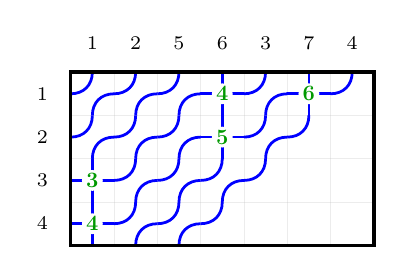
\begin{tikzpicture}[scale=0.55]
  \draw[lightgray, very thin, opacity=0.3] (0,3) -- (7,3);
  \draw[lightgray, very thin, opacity=0.3] (0,4) -- (7,4);
  \draw[lightgray, very thin, opacity=0.3] (0,5) -- (7,5);
  \draw[lightgray, very thin, opacity=0.3] (0,6) -- (7,6);
  \draw[lightgray, very thin, opacity=0.3] (0,7) -- (7,7);
  \draw[lightgray, very thin, opacity=0.3] (0,3) -- (0,7);
  \draw[lightgray, very thin, opacity=0.3] (1,3) -- (1,7);
  \draw[lightgray, very thin, opacity=0.3] (2,3) -- (2,7);
  \draw[lightgray, very thin, opacity=0.3] (3,3) -- (3,7);
  \draw[lightgray, very thin, opacity=0.3] (4,3) -- (4,7);
  \draw[lightgray, very thin, opacity=0.3] (5,3) -- (5,7);
  \draw[lightgray, very thin, opacity=0.3] (6,3) -- (6,7);
  \draw[lightgray, very thin, opacity=0.3] (7,3) -- (7,7);
  \draw[blue, line width=1.0pt] (0,6.5) .. controls (0.3,6.5) and (0.5,6.7) .. (0.5,7);
  \draw[blue, line width=1.0pt] (0.5,6) .. controls (0.5,6.3) and (0.7,6.5) .. (1,6.5);
  \draw[blue, line width=1.0pt] (1,6.5) .. controls (1.3,6.5) and (1.5,6.7) .. (1.5,7);
  \draw[blue, line width=1.0pt] (1.5,6) .. controls (1.5,6.3) and (1.7,6.5) .. (2,6.5);
  \draw[blue, line width=1.0pt] (2,6.5) .. controls (2.3,6.5) and (2.5,6.7) .. (2.5,7);
  \draw[blue, line width=1.0pt] (2.5,6) .. controls (2.5,6.3) and (2.7,6.5) .. (3,6.5);
  \draw[blue, line width=1.0pt, line cap=round] (3,6.5) -- (4,6.5);
  \draw[blue, line width=1.0pt, line cap=round] (3.5,6) -- (3.5,7);
  \draw[blue, line width=1.0pt] (4,6.5) .. controls (4.3,6.5) and (4.5,6.7) .. (4.5,7);
  \draw[blue, line width=1.0pt] (4.5,6) .. controls (4.5,6.3) and (4.7,6.5) .. (5,6.5);
  \draw[blue, line width=1.0pt, line cap=round] (5,6.5) -- (6,6.5);
  \draw[blue, line width=1.0pt, line cap=round] (5.5,6) -- (5.5,7);
  \draw[blue, line width=1.0pt] (6,6.5) .. controls (6.3,6.5) and (6.5,6.7) .. (6.5,7);
  \draw[blue, line width=1.0pt] (0,5.5) .. controls (0.3,5.5) and (0.5,5.7) .. (0.5,6);
  \draw[blue, line width=1.0pt] (0.5,5) .. controls (0.5,5.3) and (0.7,5.5) .. (1,5.5);
  \draw[blue, line width=1.0pt] (1,5.5) .. controls (1.3,5.5) and (1.5,5.7) .. (1.5,6);
  \draw[blue, line width=1.0pt] (1.5,5) .. controls (1.5,5.3) and (1.7,5.5) .. (2,5.5);
  \draw[blue, line width=1.0pt] (2,5.5) .. controls (2.3,5.5) and (2.5,5.7) .. (2.5,6);
  \draw[blue, line width=1.0pt] (2.5,5) .. controls (2.5,5.3) and (2.7,5.5) .. (3,5.5);
  \draw[blue, line width=1.0pt, line cap=round] (3,5.5) -- (4,5.5);
  \draw[blue, line width=1.0pt, line cap=round] (3.5,5) -- (3.5,6);
  \draw[blue, line width=1.0pt] (4,5.5) .. controls (4.3,5.5) and (4.5,5.7) .. (4.5,6);
  \draw[blue, line width=1.0pt] (4.5,5) .. controls (4.5,5.3) and (4.7,5.5) .. (5,5.5);
  \draw[blue, line width=1.0pt] (5,5.5) .. controls (5.3,5.5) and (5.5,5.7) .. (5.5,6);
  \draw[blue, line width=1.0pt, line cap=round] (0,4.5) -- (1,4.5);
  \draw[blue, line width=1.0pt, line cap=round] (0.5,4) -- (0.5,5);
  \draw[blue, line width=1.0pt] (1,4.5) .. controls (1.3,4.5) and (1.5,4.7) .. (1.5,5);
  \draw[blue, line width=1.0pt] (1.5,4) .. controls (1.5,4.3) and (1.7,4.5) .. (2,4.5);
  \draw[blue, line width=1.0pt] (2,4.5) .. controls (2.3,4.5) and (2.5,4.7) .. (2.5,5);
  \draw[blue, line width=1.0pt] (2.5,4) .. controls (2.5,4.3) and (2.7,4.5) .. (3,4.5);
  \draw[blue, line width=1.0pt] (3,4.5) .. controls (3.3,4.5) and (3.5,4.7) .. (3.5,5);
  \draw[blue, line width=1.0pt] (3.5,4) .. controls (3.5,4.3) and (3.7,4.5) .. (4,4.5);
  \draw[blue, line width=1.0pt] (4,4.5) .. controls (4.3,4.5) and (4.5,4.7) .. (4.5,5);
  \draw[blue, line width=1.0pt, line cap=round] (0,3.5) -- (1,3.5);
  \draw[blue, line width=1.0pt, line cap=round] (0.5,3) -- (0.5,4);
  \draw[blue, line width=1.0pt] (1,3.5) .. controls (1.3,3.5) and (1.5,3.7) .. (1.5,4);
  \draw[blue, line width=1.0pt] (1.5,3) .. controls (1.5,3.3) and (1.7,3.5) .. (2,3.5);
  \draw[blue, line width=1.0pt] (2,3.5) .. controls (2.3,3.5) and (2.5,3.7) .. (2.5,4);
  \draw[blue, line width=1.0pt] (2.5,3) .. controls (2.5,3.3) and (2.7,3.5) .. (3,3.5);
  \draw[blue, line width=1.0pt] (3,3.5) .. controls (3.3,3.5) and (3.5,3.7) .. (3.5,4);
  \node[font=\Large\bfseries, text=green!60!black, fill=white, inner sep=0.5pt, circle, transform shape] at (3.5,5.5) {5};
  \node[font=\Large\bfseries, text=green!60!black, fill=white, inner sep=0.5pt, circle, transform shape] at (0.5,4.5) {3};
  \node[font=\Large\bfseries, text=green!60!black, fill=white, inner sep=0.5pt, circle, transform shape] at (3.5,6.5) {4};
  \node[font=\Large\bfseries, text=green!60!black, fill=white, inner sep=0.5pt, circle, transform shape] at (5.5,6.5) {6};
  \node[font=\Large\bfseries, text=green!60!black, fill=white, inner sep=0.5pt, circle, transform shape] at (0.5,3.5) {4};
  \node[font=\scriptsize, text=black, anchor=south] at (0.5,7.3) {1};
  \node[font=\scriptsize, text=black, anchor=south] at (1.5,7.3) {2};
  \node[font=\scriptsize, text=black, anchor=south] at (2.5,7.3) {5};
  \node[font=\scriptsize, text=black, anchor=south] at (3.5,7.3) {6};
  \node[font=\scriptsize, text=black, anchor=south] at (4.5,7.3) {3};
  \node[font=\scriptsize, text=black, anchor=south] at (5.5,7.3) {7};
  \node[font=\scriptsize, text=black, anchor=south] at (6.5,7.3) {4};
  \node[font=\scriptsize, text=black, anchor=east] at (-0.3,6.5) {1};
  \node[font=\scriptsize, text=black, anchor=east] at (-0.3,5.5) {2};
  \node[font=\scriptsize, text=black, anchor=east] at (-0.3,4.5) {3};
  \node[font=\scriptsize, text=black, anchor=east] at (-0.3,3.5) {4};
  \draw[black, line width=1.2000000000000002pt] (0,3) rectangle (7,7);
\end{tikzpicture}}}
\end{align*}


\end{example}


% \subsection{Generating the RC graph ring}
% \newcommand{\BRCC}{\overline{\BRC}}
% % multiplying by empty row ordering
% We enlarge the module $\BRC$ to include bounded RC graphs $R$ with $\hr(R)=n$ that do not necessarily satisfy the condition that $\maxd(\wof{R})\leq n$, only that $R$ has at most $n$ rows. We denote this larger module by $\BRCC$. For $(R, p)\in \BRCC$, define $(R, p)^T\in \BRC$ by $(R^T,\maxd(\wof{R}^{-1}))$. We may define an associative product on $\BRCC$ by
% $$(R_1, p)\spadesuit(R_2,q) = \mathtt{sz}_{p+q}(((R_1, p)^T\diamond (R_2, q)^T)^T)$$
% where $\mathtt{sz}_n:\BRCC\to \BRCC$ is defined on basis elements by 
% $$\mathtt{sz}_n(R, m) = \begin{cases}(R, n) & \text{if } i\leq n\text{ for all }(i, j)\in R\\
% 0 & \text{otherwise}\end{cases}$$


\begin{definition}
Let $\mathcal{R}$  be the subring generated by the single-row RC graphs $\mathtt{row}(i)$ for $i\geq 0$. Let $a$ be a sequence of elements of a ring indexed by the nonnegative integers. For a permutation $w$ and an integer $n\geq \maxd(w)$, define a function $\dsch_w^n(a)$ By
$$\dsch_w^n(a) = \sum_{\alpha} d_{\alpha, w}^n a_{\alpha_1} \cdots a_{\alpha_n}$$
where the sum is over all weak compositions $\alpha$ of length $n$, and $d_{\alpha, w}^n$ is the coefficient of $\alpha$ in $\dsch_w^n\in\dcoma$.
\end{definition}

\begin{proposition}
We have that the elements
$$\dsch_w^n(\mathtt{row})$$
as $n$ ranges over all nonnegative integers $w$ ranges over all permutations in $S_\infty$ with $n\geq \maxd(w)$ form a $\mathbb{Z}$-basis of $\mathcal{R}$, and $\alpha:\mathcal{R}\to \dcoma$ is an isomorphism of graded rings.
\end{proposition}
\begin{proof}
Since $\alpha(\dsch_w(\mathtt{row})) = \dsch_w^n\in \dcoma$, the elements $\dsch_w^n(\mathtt{row})$ are linearly independent. Given that the images form a basis of $\dcoma$, they must also span $\mathcal{R}$ since $\dcoma$ is a free algebra, and hence there is a homomorphism backwards $\dcoma\to \mathcal{R}$ sending $[i]\mapsto \mathtt{row}(i)$ which is necessarily surjective. Thus, the elements $\dsch_w^n(\mathtt{row})$ form a $\mathbb{Z}$-basis of $\mathcal{R}$.
\end{proof}

\begin{definition}
Let $\mathcal{C}$ be the two-sided ideal generated by differences
$$R_1 - R_2$$
where $\wof{R_1}=\wof{R_2}$ and $\hr(R_1)=\hr(R_2)$. 

An element of $\mathcal{C}$ is called a \emph{chute move element} if $R_1$ and $R_2$ differ by a single chute move. It is not difficult to see that the ideal $\mathcal{C}$ is generated by chute move elements, at least as an ideal, since any two RC graphs with the same permutation and number of rows are connected by a sequence of chute moves by \cite[Theorem~3.7]{bbrc}. We may distinguish between \emph{crystal chute move elements}, where $R_2=f_i(R_1)$ for some $i$, and \emph{transition chute move elements}, where $R_2$ is obtained from $R_1$ by a chute move that is not realized by a crystal operator. 

\end{definition}

% We can classify the transition chute moves further.
It is known that the transitive closure of the relation $R_1\leq R_2$ if $R_1$ is the result of apply a chute move to $R_2$ is a partial order on the set of RC graphs for a fixed permutation and number of rows. For an RC graph $R$, we define $C(R)$ to be the difference $R - L(R)$. Transition elements are $L(R) - P(R)$.

MULTICRYSTAL RAISING/LOWERING OPERATORS
% \begin{proposition}

% \end{proposition}

By definition of the product, both crystal and transition chute move elements are preserved by left multiplication. By Theorem \ref{theorem:zcrystal}, it is clear that crystal chute move elements are preserved by right multiplication. It is less clear, but also true, that transition chute move elements are also preserved by right multiplication. 

\begin{lemma}
Suppose $R_1$ and $R_2$ differ by a single chute move at row $i$. Then for any RC graph $R$, the elements $(R_1 - R_2)\diamond R$ and $R\diamond (R_1 - R_2)$ are sums of chute move elements.
\end{lemma}
\begin{proof}
For left muliplication, $R_1$ and $R_2$ are actually subgraphs of all resulting elements. For right multiplication, let $R'$ be an RC graph in the product. Then there is a crystal isomorphism between a subset of the crystal components of RC graphs for $\wof{R'}$ and the entirety of the crystal components of RC graphs for $\wof{R_1}=\wof{R_2}$. Note that the chute moves form a basis over $\mathbb{Z}$, and hence over $\mathbb{Q}$. Thus, applying the right inverse map $\zeromap$, $R_1 - R_2$ restricted to a single permutation map to an element $R_1' - R_2'$, which necessarily is a sum of chute moves
\end{proof}


\begin{theorem}
  $\BRC$ decomposes as an internal direct sum
  $$\mathcal{R}\oplus \mathcal{C}$$
  and $\mathcal{C}$ is an $(\mathcal{R},\mathcal{R})$-bimodule generated by the chute move elements that is free as a left $\mathcal{R}$-module.
\end{theorem}
\begin{proof}
For any RC grapn with $n$ rows for a permutation $w$, we have $\alpha(\dsch_w^n(\mathtt{row})) = \alpha(R)$, so that $\dsch_w^n(\mathtt{row}) - R\in \mathcal{C}$. It follows that
$$\mathcal{R}+\mathcal{C}=\BRC$$ 
and that $\mathcal{R}\cap \mathcal{C} = 0$ since $\alpha$ is injective on $\mathcal{R}$ and vanishes on $\mathcal{C}$.
\end{proof}

\newcommand{\gra}{\mathrm{gr}_{\mathcal{C}}(\BRC)}
Let us consider the associated graded ring $\gra$ with respect to the filtration induced by the ideal $\mathcal{C}$. We can view the degree $k$ component as an RC graph $R$ together with a choice of $k$ rightmost simple chute moves in disjoint adjacent pairs of rows. Thus the degree $0$ component is isomorphic to $\dcoma$, whereas each higher component has more specificity with certain pairs of rows constrained to specific chute moves.
%There is a combinatorial description of the degree $k$ component: they correspond to formal linear combinations of equivalence classes of RC graphs where there are indices $a_1,\ldots,a_k$, where $a_{i+1} - a_{i}\geq 2$, of chute moves at row $a_i$ that can be applied to any representative of the equivalence class.
\begin{theorem}
The associated graded ring $\gra$ has as a basis for its $k$th graded component equivalence classes of differences of RC graphs by applying $k$ simultaneous rightmost simple chute moves (so that only those $2k$ rows are specifically identified).
\end{theorem}

Define a sequence $\wtt^*(R)$ to be the weight of $R^T$.

\begin{lemma}
  The map $R\mapsto R^T$ is an isomorphism of Demazure crystals with the conjugate highest weight. Specifically, $\mathcal{C}(R^T)\cong \mathcal{C}(R)^\#$.
\end{lemma}
\newcommand{\ltb}{\mathrm{little}}
\newcommand{\ls}{\mathrm{LS}}
\newcommand{\hw}{\mathbb{Y}}
\newcommand{\ww}{\mathbb{W}}
\begin{definition}
Define a module $\hw(\BRC)$ by letting $\hw(\BRC) = \{\hw(R): R\in \BRC\}$ with the obvious scalar multiplication. Define also a bilinear product on $\hw(\BRC)$ by
$$\hw(R_1)\cdot \hw(R_2) = \hw(\hw(R_1)\diamond \hw(R_2))$$

Define an ideal $Y\subseteq \BRC$ to be the ideal generated by the elements
$$R - \hw(R)$$
Then $\hw:\BRC\to\hw(\BRC)$ is a homomorphism of rings.

Is squash inserting?

Yes squash product is left insertion into the highest weight-tableau representation.

Define a ring $\ww(\BRC)$ and function
$$\ww:\BRC\to \ww(\BRC)$$
such that if
$$R = F\hw(R)$$
then
$$\ww(R) = F\hw(B(\wtt(R)))$$
$\ww(\BRC)$ also has a product defined by
$$R_1\cdot R_2 = \sum_{R\in \ww(\BRC)}c_RR$$
where $c_R$ is the coefficient of $R$ in the expansion of $R_1\diamond R_2$ in the basis of $\BRC$.

Then 
$$\hw\otimes \ww\to \hw(\BRC)\otimes \ww(\BRC)$$
is an injective homomorphism of rings. 

Note: $\ww:\BRC\to \ww(\BRC)$ is not a homomorphism of rings.
\end{definition}



\subsection{Relation to Little bumps}


\newcommand{\lzeromap}{\mathscr{Z}}
\newcommand{\lmap}{\mathscr{L}}
Define a function $\lmap:\BRC^0(n)\to\BRC(n+1)$ as follows. Assume $n=\maxd(\wof{R})$, and suppose $\rtt_R(i, j) = (n, n + 1)$, where $i < n$. Set 
$$R'= (R\setminus \{(i, j)\})\cup \{(n,1)\}$$
Then define
$$\lmap(R, n) = ((\ins{n-1}{i} R')\setminus\{(n, 1)\}, n + 1)$$
Then define $\lzeromap:\BRC^0(n)\to \BRC(n-1)$ by iterating $\lmap$ and stopping as soon as the result has $\maxd(\wof{R})\leq n-1$.

\begin{proposition} \label{proposition:little_bump}
  Let $(R, n)\in \BRC^0(n)$ be a bounded RC graph such that $\maxd(\wof{R}) = n$. Suppose 
  $$\mathrm{word}(R) = a_1 a_2 \cdots a_k$$ 
  and 
  $$\mathrm{seq}(R) = r_1 r_2 \cdots r_k$$ 
  suppose $\rtt_R(i,j)=(n,n+1)$, and let $p$ be the index such that $r_p=i$ and $r_p + j - 1 = a_p$. Then
  $$\mathrm{word}(\lmap(R, n)) = \ltb_{p}(\mathrm{word}(R, n))$$
\end{proposition}
\begin{proof}
Consider the biword
$$\begin{matrix}
r_1& r_2& \cdots & r_{p-1} & r_p & r_{p+1} & \cdots & r_k\\
a_1& a_2& \cdots & a_{p-1} & a_p & a_{p+1} & \cdots & a_k
\end{matrix}$$
The first deletion yields
$$\begin{matrix}
r_1& r_2& \cdots & r_{p-1} &  r_{p+1} & \cdots & r_k& n\\
a_1& a_2& \cdots & a_{p-1} &  a_{p+1} & \cdots & a_k& n
\end{matrix}$$
Necessarily, we must have $a_p > 1$. If we have $a_p=1$, then we would have $r_p=1$. The only way for position $(1,1)$ in an RC graph to be a right descent is if it is the unique right descent. By assumption, that descent would have to be $n$, so that $n=1$. In that case, however, it would not be possible for the last row to be empty. 

We also must have that $r_p < a_p$, because there is a sequence of chute moves involving this crossing that moves it to position $(n, 1)$ by \cite[Theorem~3.7]{bbrc}. Assume first that $p = k$. Then the insertion algorithm will insert $a_p - 1=n-1$ into row $r_k$. If this word is reduced, then we are done, and this clearly coincides with the Little bump. If it is not reduced, the descent $n-1$ occurs somewhere to the left, say at position $j$. The insertion algorithm would delete this letter then try to insert another one. However, we can see that recursively this is the same as applying $\zeromap_+$ to the biword obtained by removing all letters after position $j$ and then reinserting them afterwards. By the inductive hypothesis, this coincides with applying the Little bump at position $j$, which would indeed be the next step in the recursion of applying the Little bump at position $k$. Thus, the two coincide by induction.
\end{proof}

\begin{theorem}[{\cite[Theorem~4.4]{hamaker2014relating}}]
Let $\mathrm{w}$ be a reduced word for a permutation $w\in S_\infty$. Then
$$Q(\mathrm{w}) = Q(\ltb_p(\mathrm{w}))$$
for any valid $p$.
\end{theorem}

\begin{corollary}
  $\lmap:\BRC^0(n)\to \BRC(n+1)$ is a weight-preserving injection that preserves the recording tableau under the Edelman-Greene correspondence.
\end{corollary}

\begin{corollary}
$$\lzeromap:\RC(w, n)^0\to \bigcup_{w\downvar{n} w'}\RC(w', n-1)$$ 
	is a weight-preserving isomorphism of crystal graphs.
\end{corollary}


\begin{corollary}
  We have the equality
$$\lzeromap=\zeromap$$ 
\end{corollary}


\subsection{Relation to the bijection with bumpless pipe dreams}

\newcommand{\BPD}{\mathcal{BPD}}


\begin{definition}
  Denote by $\BPD(w,n)$ the set of (reduced) $n$-row bumpless pipe dreams for a permutation $w$, where $n\geq \maxd(w)$. These are $n\times N$ grids, where $N$ is at least the length of $w$, populated with $6$ possible tiles, shown in Figure \ref{figure:bpdtiles}, satisfying the conditions that pipes must enter from the bottom and exit on the right, and no two pipes may cross twice. We may assign a permutation to such a BPD as follows.

  Let $(B, n)$ be an $n$-row BPD. Let $c_1,\ldots,c_m$ be the columns such that the pipes on the bottom edge have an entrance from the bottom. If the pipe coming from $c_i$ exits on row $j$ on the right, then $w(c_i) = j$. To fill in the remaining elements of the permutation, we set $w(m + k) = d_k$, where $d_1,\ldots,d_k$ are the remaining columns with no entrance in increasing order.

  

\end{definition}

\begin{figure}[htbp]
\centering
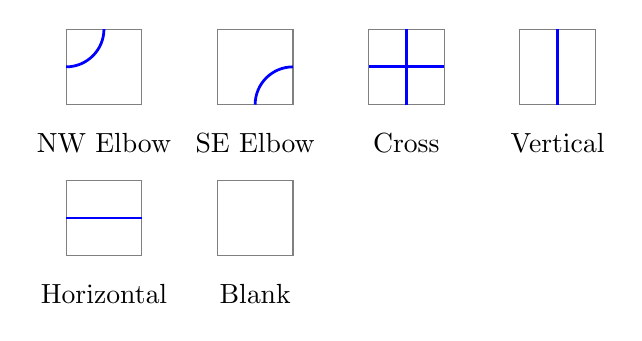
\begin{tikzpicture}[scale=0.8]
% Define common parameters
\def\tilesize{1.2}
\def\pipewidth{1pt}

% Tile 1: NW Elbow
\begin{scope}[shift={(0,0)}]
  \draw[gray] (0,0) rectangle (\tilesize,\tilesize);
  \draw[line width=\pipewidth, blue] (0,0.5*\tilesize) 
    arc[start angle=-90, end angle=0, radius=0.5*\tilesize];
  \node[below] at (0.5*\tilesize,-0.3) {NW Elbow};
\end{scope}

% Tile 2: SE Elbow
\begin{scope}[shift={(2*\tilesize,0)}]
  \draw[gray] (0,0) rectangle (\tilesize,\tilesize);
  \draw[line width=\pipewidth, blue] (0.5*\tilesize,0) 
    arc[start angle=180, end angle=90, radius=0.5*\tilesize];
  \node[below] at (0.5*\tilesize,-0.3) {SE Elbow};
\end{scope}

% Tile 3: Cross
\begin{scope}[shift={(4*\tilesize,0)}]
  \draw[gray] (0,0) rectangle (\tilesize,\tilesize);
  \draw[line width=\pipewidth, blue] (0,0.5*\tilesize) -- (\tilesize,0.5*\tilesize);
  \draw[line width=\pipewidth, blue] (0.5*\tilesize,0) -- (0.5*\tilesize,\tilesize);
  \node[below] at (0.5*\tilesize,-0.3) {Cross};
\end{scope}

% Tile 4: Vertical
\begin{scope}[shift={(6*\tilesize,0)}]
  \draw[gray] (0,0) rectangle (\tilesize,\tilesize);
  \draw[line width=\pipewidth, blue] (0.5*\tilesize,0) -- (0.5*\tilesize,\tilesize);
  \node[below] at (0.5*\tilesize,-0.3) {Vertical};
\end{scope}

% Tile 5: Horizontal
\begin{scope}[shift={(0,-2*\tilesize)}]
  \draw[gray] (0,0) rectangle (\tilesize,\tilesize);
  \draw[line width=\pipewidth, blue] (0,0.5*\tilesize) -- (\tilesize,0.5*\tilesize);
  \node[below] at (0.5*\tilesize,-0.3) {Horizontal};
\end{scope}

% Tile 6: Blank
\begin{scope}[shift={(2*\tilesize,-2*\tilesize)}]
  \draw[gray] (0,0) rectangle (\tilesize,\tilesize);
  \node[below] at (0.5*\tilesize,-0.3) {Blank};
\end{scope}

\end{tikzpicture}
\caption{The six possible tiles in bumpless pipe dreams. Pipes enter from the bottom and exit at the right.}
\label{figure:bpdtiles}
\end{figure}


\begin{lemma}[{\cite[Theorem~3.6]{Yu2025EmbeddingBP}}] \label{lemma:bpd_completion}
  Let $(B, N)$ be an ordinary reduced BPD for a permutation $w$, so that $w(M) = M$ for all $M>N$ and $B$ is $N\times N$. Let $n\geq \maxd(w)$ be an integer. Then the BPD $B'$ obtained by only retaining the first $n$ rows of $B$ satisfies $w(B', n) = w(B, N)$ and uniquely determines $B$ under this assumption.
\end{lemma}


\begin{definition}
There is a bijection $\varphi:\BPD(w,n)\to \mathcal{RC}(w,n)$, where $w\in S_n$, defined in \cite{GaoHuang2023} that preserves weight. It is viewed as ``canonical'' because it also provides bijective correspondences between certain insertion/bumping operations on BPDs and RC graphs, showing that they agree in a strong way. In light of Lemma \ref{lemma:bpd_completion}, we may extend this bijection to $w\in S_\infty$ with $\maxd(w)\leq n$ by first expanding the BPD to a square BPD with sufficiently many rows and columns, then applying the bijection, and finally truncating the resulting RC graph to $n$ rows.
\end{definition}

\begin{figure}[htbp]
\centering
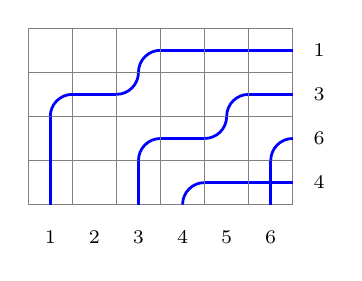
\begin{tikzpicture}[scale=0.7]
\def\s{0.8}  % tile size
\def\pw{1pt} % pipe width

% Row 0 (bottom): vert, blank, vert, se, horiz, cross
% Col 0: vertical
\draw[gray] (0,0) rectangle (\s,\s);
\draw[line width=\pw, blue] (0.5*\s,0) -- (0.5*\s,\s);
% Col 1: blank
\draw[gray] (\s,0) rectangle (2*\s,\s);
% Col 2: vertical
\draw[gray] (2*\s,0) rectangle (3*\s,\s);
\draw[line width=\pw, blue] (2.5*\s,0) -- (2.5*\s,\s);
% Col 3: se elbow
\draw[gray] (3*\s,0) rectangle (4*\s,\s);
\draw[line width=\pw, blue] (3.5*\s,0) arc[start angle=180, end angle=90, radius=0.5*\s];
% Col 4: horizontal
\draw[gray] (4*\s,0) rectangle (5*\s,\s);
\draw[line width=\pw, blue] (4*\s,0.5*\s) -- (5*\s,0.5*\s);
% Col 5: cross
\draw[gray] (5*\s,0) rectangle (6*\s,\s);
\draw[line width=\pw, blue] (5*\s,0.5*\s) -- (6*\s,0.5*\s);
\draw[line width=\pw, blue] (5.5*\s,0) -- (5.5*\s,\s);

% Row 1: vert, blank, se, horiz, nw, se
% Col 0: vertical
\draw[gray] (0,\s) rectangle (\s,2*\s);
\draw[line width=\pw, blue] (0.5*\s,\s) -- (0.5*\s,2*\s);
% Col 1: blank
\draw[gray] (\s,\s) rectangle (2*\s,2*\s);
% Col 2: se elbow
\draw[gray] (2*\s,\s) rectangle (3*\s,2*\s);
\draw[line width=\pw, blue] (2.5*\s,\s) arc[start angle=180, end angle=90, radius=0.5*\s];
% Col 3: horizontal
\draw[gray] (3*\s,\s) rectangle (4*\s,2*\s);
\draw[line width=\pw, blue] (3*\s,1.5*\s) -- (4*\s,1.5*\s);
% Col 4: nw elbow
\draw[gray] (4*\s,\s) rectangle (5*\s,2*\s);
\draw[line width=\pw, blue] (4*\s,1.5*\s) arc[start angle=-90, end angle=0, radius=0.5*\s];
% Col 5: se elbow
\draw[gray] (5*\s,\s) rectangle (6*\s,2*\s);
\draw[line width=\pw, blue] (5.5*\s,\s) arc[start angle=180, end angle=90, radius=0.5*\s];

% Row 2: se, horiz, nw, blank, se, horiz
% Col 0: se elbow
\draw[gray] (0,2*\s) rectangle (\s,3*\s);
\draw[line width=\pw, blue] (0.5*\s,2*\s) arc[start angle=180, end angle=90, radius=0.5*\s];
% Col 1: horizontal
\draw[gray] (\s,2*\s) rectangle (2*\s,3*\s);
\draw[line width=\pw, blue] (\s,2.5*\s) -- (2*\s,2.5*\s);
% Col 2: nw elbow
\draw[gray] (2*\s,2*\s) rectangle (3*\s,3*\s);
\draw[line width=\pw, blue] (2*\s,2.5*\s) arc[start angle=-90, end angle=0, radius=0.5*\s];
% Col 3: blank
\draw[gray] (3*\s,2*\s) rectangle (4*\s,3*\s);
% Col 4: se elbow
\draw[gray] (4*\s,2*\s) rectangle (5*\s,3*\s);
\draw[line width=\pw, blue] (4.5*\s,2*\s) arc[start angle=180, end angle=90, radius=0.5*\s];
% Col 5: horizontal
\draw[gray] (5*\s,2*\s) rectangle (6*\s,3*\s);
\draw[line width=\pw, blue] (5*\s,2.5*\s) -- (6*\s,2.5*\s);

% Row 3 (top): blank, blank, se, horiz, horiz, horiz
% Col 0: blank
\draw[gray] (0,3*\s) rectangle (\s,4*\s);
% Col 1: blank
\draw[gray] (\s,3*\s) rectangle (2*\s,4*\s);
% Col 2: se elbow
\draw[gray] (2*\s,3*\s) rectangle (3*\s,4*\s);
\draw[line width=\pw, blue] (2.5*\s,3*\s) arc[start angle=180, end angle=90, radius=0.5*\s];
% Col 3: horizontal
\draw[gray] (3*\s,3*\s) rectangle (4*\s,4*\s);
\draw[line width=\pw, blue] (3*\s,3.5*\s) -- (4*\s,3.5*\s);
% Col 4: horizontal
\draw[gray] (4*\s,3*\s) rectangle (5*\s,4*\s);
\draw[line width=\pw, blue] (4*\s,3.5*\s) -- (5*\s,3.5*\s);
% Col 5: horizontal
\draw[gray] (5*\s,3*\s) rectangle (6*\s,4*\s);
\draw[line width=\pw, blue] (5*\s,3.5*\s) -- (6*\s,3.5*\s);

% Column labels at bottom
\foreach \i in {1,...,6} {
  \node[below] at (\i*\s-0.5*\s,-0.3) {\scriptsize \i};
}

% Row exit labels on right
\node[right] at (6*\s+0.2,3.5*\s) {\scriptsize 1};
\node[right] at (6*\s+0.2,2.5*\s) {\scriptsize 3};
\node[right] at (6*\s+0.2,1.5*\s) {\scriptsize 6};
\node[right] at (6*\s+0.2,0.5*\s) {\scriptsize 4};

\end{tikzpicture}

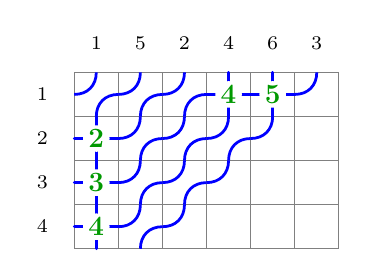
\begin{tikzpicture}[scale=0.7]
  \def\s{0.8}
  \draw[gray] (0,\s) -- (6*\s,\s);
  \draw[gray] (0,\s) -- (0,5*\s);
  \draw[gray] (0,2*\s) -- (6*\s,2*\s);
  \draw[gray] (\s,\s) -- (\s,5*\s);
  \draw[gray] (0,3*\s) -- (6*\s,3*\s);
  \draw[gray] (2*\s,\s) -- (2*\s,5*\s);
  \draw[gray] (0,4*\s) -- (6*\s,4*\s);
  \draw[gray] (3*\s,\s) -- (3*\s,5*\s);
  \draw[gray] (0,5*\s) -- (6*\s,5*\s);
  \draw[gray] (4*\s,\s) -- (4*\s,5*\s);
  \draw[gray] (5*\s,\s) -- (5*\s,5*\s);
  \draw[gray] (6*\s,\s) -- (6*\s,5*\s);
  \draw[blue, line width=1.0pt] (0,4.5*\s) .. controls (0.3*\s,4.5*\s) and (0.5*\s,4.7*\s) .. (0.5*\s,5*\s);
  \draw[blue, line width=1.0pt] (0.5*\s,4*\s) .. controls (0.5*\s,4.3*\s) and (0.7*\s,4.5*\s) .. (1*\s,4.5*\s);
  \draw[blue, line width=1.0pt] (1*\s,4.5*\s) .. controls (1.3*\s,4.5*\s) and (1.5*\s,4.7*\s) .. (1.5*\s,5*\s);
  \draw[blue, line width=1.0pt] (1.5*\s,4*\s) .. controls (1.5*\s,4.3*\s) and (1.7*\s,4.5*\s) .. (2*\s,4.5*\s);
  \draw[blue, line width=1.0pt] (2*\s,4.5*\s) .. controls (2.3*\s,4.5*\s) and (2.5*\s,4.7*\s) .. (2.5*\s,5*\s);
  \draw[blue, line width=1.0pt] (2.5*\s,4*\s) .. controls (2.5*\s,4.3*\s) and (2.7*\s,4.5*\s) .. (3*\s,4.5*\s);
  \draw[blue, line width=1.0pt, line cap=round] (3*\s,4.5*\s) -- (4*\s,4.5*\s);
  \draw[blue, line width=1.0pt, line cap=round] (3.5*\s,4*\s) -- (3.5*\s,5*\s);
  \draw[blue, line width=1.0pt, line cap=round] (4*\s,4.5*\s) -- (5*\s,4.5*\s);
  \draw[blue, line width=1.0pt, line cap=round] (4.5*\s,4*\s) -- (4.5*\s,5*\s);
  \draw[blue, line width=1.0pt] (5*\s,4.5*\s) .. controls (5.3*\s,4.5*\s) and (5.5*\s,4.7*\s) .. (5.5*\s,5*\s);
  \draw[blue, line width=1.0pt, line cap=round] (0,3.5*\s) -- (1*\s,3.5*\s);
  \draw[blue, line width=1.0pt, line cap=round] (0.5*\s,3*\s) -- (0.5*\s,4*\s);
  \draw[blue, line width=1.0pt] (1*\s,3.5*\s) .. controls (1.3*\s,3.5*\s) and (1.5*\s,3.7*\s) .. (1.5*\s,4*\s);
  \draw[blue, line width=1.0pt] (1.5*\s,3*\s) .. controls (1.5*\s,3.3*\s) and (1.7*\s,3.5*\s) .. (2*\s,3.5*\s);
  \draw[blue, line width=1.0pt] (2*\s,3.5*\s) .. controls (2.3*\s,3.5*\s) and (2.5*\s,3.7*\s) .. (2.5*\s,4*\s);
  \draw[blue, line width=1.0pt] (2.5*\s,3*\s) .. controls (2.5*\s,3.3*\s) and (2.7*\s,3.5*\s) .. (3*\s,3.5*\s);
  \draw[blue, line width=1.0pt] (3*\s,3.5*\s) .. controls (3.3*\s,3.5*\s) and (3.5*\s,3.7*\s) .. (3.5*\s,4*\s);
  \draw[blue, line width=1.0pt] (3.5*\s,3*\s) .. controls (3.5*\s,3.3*\s) and (3.7*\s,3.5*\s) .. (4*\s,3.5*\s);
  \draw[blue, line width=1.0pt] (4*\s,3.5*\s) .. controls (4.3*\s,3.5*\s) and (4.5*\s,3.7*\s) .. (4.5*\s,4*\s);
  \draw[blue, line width=1.0pt, line cap=round] (0,2.5*\s) -- (1*\s,2.5*\s);
  \draw[blue, line width=1.0pt, line cap=round] (0.5*\s,2*\s) -- (0.5*\s,3*\s);
  \draw[blue, line width=1.0pt] (1*\s,2.5*\s) .. controls (1.3*\s,2.5*\s) and (1.5*\s,2.7*\s) .. (1.5*\s,3*\s);
  \draw[blue, line width=1.0pt] (1.5*\s,2*\s) .. controls (1.5*\s,2.3*\s) and (1.7*\s,2.5*\s) .. (2*\s,2.5*\s);
  \draw[blue, line width=1.0pt] (2*\s,2.5*\s) .. controls (2.3*\s,2.5*\s) and (2.5*\s,2.7*\s) .. (2.5*\s,3*\s);
  \draw[blue, line width=1.0pt] (2.5*\s,2*\s) .. controls (2.5*\s,2.3*\s) and (2.7*\s,2.5*\s) .. (3*\s,2.5*\s);
  \draw[blue, line width=1.0pt] (3*\s,2.5*\s) .. controls (3.3*\s,2.5*\s) and (3.5*\s,2.7*\s) .. (3.5*\s,3*\s);
  \draw[blue, line width=1.0pt, line cap=round] (0,1.5*\s) -- (1*\s,1.5*\s);
  \draw[blue, line width=1.0pt, line cap=round] (0.5*\s,1*\s) -- (0.5*\s,2*\s);
  \draw[blue, line width=1.0pt] (1*\s,1.5*\s) .. controls (1.3*\s,1.5*\s) and (1.5*\s,1.7*\s) .. (1.5*\s,2*\s);
  \draw[blue, line width=1.0pt] (1.5*\s,1*\s) .. controls (1.5*\s,1.3*\s) and (1.7*\s,1.5*\s) .. (2*\s,1.5*\s);
  \draw[blue, line width=1.0pt] (2*\s,1.5*\s) .. controls (2.3*\s,1.5*\s) and (2.5*\s,1.7*\s) .. (2.5*\s,2*\s);
  \node[font=\Large\bfseries, text=green!60!black, fill=white, inner sep=0.5pt, circle, transform shape] at (0.5*\s,3.5*\s) {2};
  \node[font=\Large\bfseries, text=green!60!black, fill=white, inner sep=0.5pt, circle, transform shape] at (4.5*\s,4.5*\s) {5};
  \node[font=\Large\bfseries, text=green!60!black, fill=white, inner sep=0.5pt, circle, transform shape] at (0.5*\s,2.5*\s) {3};
  \node[font=\Large\bfseries, text=green!60!black, fill=white, inner sep=0.5pt, circle, transform shape] at (3.5*\s,4.5*\s) {4};
  \node[font=\Large\bfseries, text=green!60!black, fill=white, inner sep=0.5pt, circle, transform shape] at (0.5*\s,1.5*\s) {4};
  \node[font=\scriptsize, text=black, anchor=south] at (0.5*\s,5.3*\s) {1};
  \node[font=\scriptsize, text=black, anchor=south] at (1.5*\s,5.3*\s) {5};
  \node[font=\scriptsize, text=black, anchor=south] at (2.5*\s,5.3*\s) {2};
  \node[font=\scriptsize, text=black, anchor=south] at (3.5*\s,5.3*\s) {4};
  \node[font=\scriptsize, text=black, anchor=south] at (4.5*\s,5.3*\s) {6};
  \node[font=\scriptsize, text=black, anchor=south] at (5.5*\s,5.3*\s) {3};
  \node[font=\scriptsize, text=black, anchor=east] at (-0.3,4.5*\s) {1};
  \node[font=\scriptsize, text=black, anchor=east] at (-0.3,3.5*\s) {2};
  \node[font=\scriptsize, text=black, anchor=east] at (-0.3,2.5*\s) {3};
  \node[font=\scriptsize, text=black, anchor=east] at (-0.3,1.5*\s) {4};
\end{tikzpicture}
\caption{An example of a $4$-row bumpless pipe dream for a permutation of length $6$. Pipes enter from the bottom at columns 1, 3, 4, and 6, and exit on the right at the labeled rows. The associated permutation is $[1,3,6,4,2,5]$. The associated RC graph under the bijection $\varphi$ is shown as well, with crosses in positions $(1,4)$, $(1,5)$, $(2,1)$, $(3,1)$, and $(4,1)$.}
\label{figure:bpdexample}
\end{figure}

\newcommand{\bzeromap}{\mathbf{t}}


\begin{definition}
We define a function $\bzeromap:\BPD(n)^0\to \BPD(n-1)$, found in \cite{WEIGANDT2021105470} in a more general context, as follows. Given a bumpless pipe dream $(B, n)$ with no blank tiles in row $n$, we simply remove row $n$ to obtain $B'$. Then
$$\bzeromap(B, n) = (B', n-1)$$
One may ask oneself here whether anything changes at all. Indeed, all that changes are the labels of the incoming pipes, as shown in Figure \ref{figure:transition}, and this only happens if $\maxd(w) = n$.
\end{definition}






\begin{figure}[htbp]
\centering
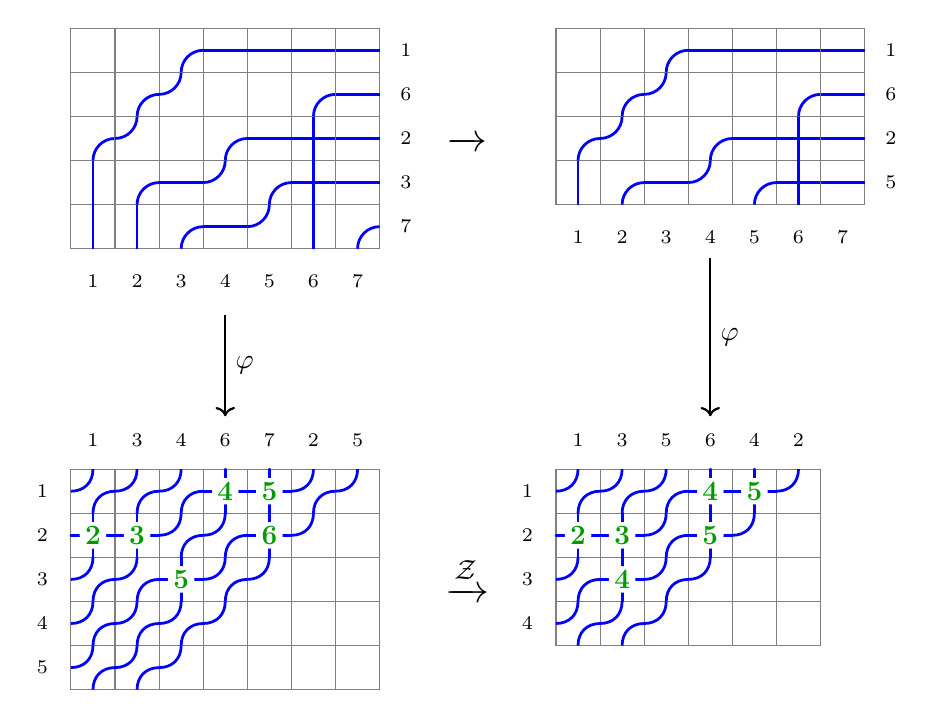
\begin{tikzpicture}[scale=0.7]
\def\s{0.8}
\def\pw{1pt}

% First BPD (left side) - 5 rows x 7 cols
\begin{scope}
% Row 0 (bottom, will be removed): VERT, VERT, SE, HORIZ, NW, VERT, SE
\draw[gray] (0,0) rectangle (\s,\s);
\draw[line width=\pw, blue] (0.5*\s,0) -- (0.5*\s,\s);
\draw[gray] (\s,0) rectangle (2*\s,\s);
\draw[line width=\pw, blue] (1.5*\s,0) -- (1.5*\s,\s);
\draw[gray] (2*\s,0) rectangle (3*\s,\s);
\draw[line width=\pw, blue] (2.5*\s,0) arc[start angle=180, end angle=90, radius=0.5*\s];
\draw[gray] (3*\s,0) rectangle (4*\s,\s);
\draw[line width=\pw, blue] (3*\s,0.5*\s) -- (4*\s,0.5*\s);
\draw[gray] (4*\s,0) rectangle (5*\s,\s);
\draw[line width=\pw, blue] (4*\s,0.5*\s) arc[start angle=-90, end angle=0, radius=0.5*\s];
\draw[gray] (5*\s,0) rectangle (6*\s,\s);
\draw[line width=\pw, blue] (5.5*\s,0) -- (5.5*\s,\s);
\draw[gray] (6*\s,0) rectangle (7*\s,\s);
\draw[line width=\pw, blue] (6.5*\s,0) arc[start angle=180, end angle=90, radius=0.5*\s];

% Row 1: VERT, SE, HORIZ, NW, SE, CROSS, HORIZ
\draw[gray] (0,\s) rectangle (\s,2*\s);
\draw[line width=\pw, blue] (0.5*\s,\s) -- (0.5*\s,2*\s);
\draw[gray] (\s,\s) rectangle (2*\s,2*\s);
\draw[line width=\pw, blue] (1.5*\s,\s) arc[start angle=180, end angle=90, radius=0.5*\s];
\draw[gray] (2*\s,\s) rectangle (3*\s,2*\s);
\draw[line width=\pw, blue] (2*\s,1.5*\s) -- (3*\s,1.5*\s);
\draw[gray] (3*\s,\s) rectangle (4*\s,2*\s);
\draw[line width=\pw, blue] (3*\s,1.5*\s) arc[start angle=-90, end angle=0, radius=0.5*\s];
\draw[gray] (4*\s,\s) rectangle (5*\s,2*\s);
\draw[line width=\pw, blue] (4.5*\s,\s) arc[start angle=180, end angle=90, radius=0.5*\s];
\draw[gray] (5*\s,\s) rectangle (6*\s,2*\s);
\draw[line width=\pw, blue] (5*\s,1.5*\s) -- (6*\s,1.5*\s);
\draw[line width=\pw, blue] (5.5*\s,\s) -- (5.5*\s,2*\s);
\draw[gray] (6*\s,\s) rectangle (7*\s,2*\s);
\draw[line width=\pw, blue] (6*\s,1.5*\s) -- (7*\s,1.5*\s);

% Row 2: SE, NW, BLANK, SE, HORIZ, CROSS, HORIZ
\draw[gray] (0,2*\s) rectangle (\s,3*\s);
\draw[line width=\pw, blue] (0.5*\s,2*\s) arc[start angle=180, end angle=90, radius=0.5*\s];
\draw[gray] (\s,2*\s) rectangle (2*\s,3*\s);
\draw[line width=\pw, blue] (\s,2.5*\s) arc[start angle=-90, end angle=0, radius=0.5*\s];
\draw[gray] (2*\s,2*\s) rectangle (3*\s,3*\s);
\draw[gray] (3*\s,2*\s) rectangle (4*\s,3*\s);
\draw[line width=\pw, blue] (3.5*\s,2*\s) arc[start angle=180, end angle=90, radius=0.5*\s];
\draw[gray] (4*\s,2*\s) rectangle (5*\s,3*\s);
\draw[line width=\pw, blue] (4*\s,2.5*\s) -- (5*\s,2.5*\s);
\draw[gray] (5*\s,2*\s) rectangle (6*\s,3*\s);
\draw[line width=\pw, blue] (5*\s,2.5*\s) -- (6*\s,2.5*\s);
\draw[line width=\pw, blue] (5.5*\s,2*\s) -- (5.5*\s,3*\s);
\draw[gray] (6*\s,2*\s) rectangle (7*\s,3*\s);
\draw[line width=\pw, blue] (6*\s,2.5*\s) -- (7*\s,2.5*\s);

% Row 3: BLANK, SE, NW, BLANK, BLANK, SE, HORIZ
\draw[gray] (0,3*\s) rectangle (\s,4*\s);
\draw[gray] (\s,3*\s) rectangle (2*\s,4*\s);
\draw[line width=\pw, blue] (1.5*\s,3*\s) arc[start angle=180, end angle=90, radius=0.5*\s];
\draw[gray] (2*\s,3*\s) rectangle (3*\s,4*\s);
\draw[line width=\pw, blue] (2*\s,3.5*\s) arc[start angle=-90, end angle=0, radius=0.5*\s];
\draw[gray] (3*\s,3*\s) rectangle (4*\s,4*\s);
\draw[gray] (4*\s,3*\s) rectangle (5*\s,4*\s);
\draw[gray] (5*\s,3*\s) rectangle (6*\s,4*\s);
\draw[line width=\pw, blue] (5.5*\s,3*\s) arc[start angle=180, end angle=90, radius=0.5*\s];
\draw[gray] (6*\s,3*\s) rectangle (7*\s,4*\s);
\draw[line width=\pw, blue] (6*\s,3.5*\s) -- (7*\s,3.5*\s);

% Row 4 (top): BLANK, BLANK, SE, HORIZ, HORIZ, HORIZ, HORIZ
\draw[gray] (0,4*\s) rectangle (\s,5*\s);
\draw[gray] (\s,4*\s) rectangle (2*\s,5*\s);
\draw[gray] (2*\s,4*\s) rectangle (3*\s,5*\s);
\draw[line width=\pw, blue] (2.5*\s,4*\s) arc[start angle=180, end angle=90, radius=0.5*\s];
\draw[gray] (3*\s,4*\s) rectangle (4*\s,5*\s);
\draw[line width=\pw, blue] (3*\s,4.5*\s) -- (4*\s,4.5*\s);
\draw[gray] (4*\s,4*\s) rectangle (5*\s,5*\s);
\draw[line width=\pw, blue] (4*\s,4.5*\s) -- (5*\s,4.5*\s);
\draw[gray] (5*\s,4*\s) rectangle (6*\s,5*\s);
\draw[line width=\pw, blue] (5*\s,4.5*\s) -- (6*\s,4.5*\s);
\draw[gray] (6*\s,4*\s) rectangle (7*\s,5*\s);
\draw[line width=\pw, blue] (6*\s,4.5*\s) -- (7*\s,4.5*\s);

% Column labels at bottom
\foreach \i in {1,...,7} {
  \node[below] at (\i*\s-0.5*\s,-0.3) {\scriptsize \i};
}
% Exit labels on right (showing which row each pipe exits)
\node[right] at (7*\s+0.2,0.5*\s) {\scriptsize 7};
\node[right] at (7*\s+0.2,1.5*\s) {\scriptsize 3};
\node[right] at (7*\s+0.2,2.5*\s) {\scriptsize 2};
\node[right] at (7*\s+0.2,3.5*\s) {\scriptsize 6};
\node[right] at (7*\s+0.2,4.5*\s) {\scriptsize 1};
\end{scope}

% Vertical arrow from left BPD to left RC graph
\draw[->, line width=0.8pt] (3.5*\s,-1.2) -- (3.5*\s,-3.8*\s) node[midway, right] {$\varphi$};

% Arrow and label
\node at (9*\s,2.5*\s) {\Large $\xrightarrow{\bzeromap}$};

% Second BPD (right side) - 4 rows (bottom row removed)
\begin{scope}[shift={(11*\s,\s)}]
% Start from row 1 (skipping the bottom row from left BPD)
% Row 0 (was row 1): VERT, SE, HORIZ, NW, SE, CROSS, HORIZ
\draw[gray] (0,0) rectangle (\s,\s);
\draw[line width=\pw, blue] (0.5*\s,0) -- (0.5*\s,\s);
\draw[gray] (\s,0) rectangle (2*\s,\s);
\draw[line width=\pw, blue] (1.5*\s,0) arc[start angle=180, end angle=90, radius=0.5*\s];
\draw[gray] (2*\s,0) rectangle (3*\s,\s);
\draw[line width=\pw, blue] (2*\s,0.5*\s) -- (3*\s,0.5*\s);
\draw[gray] (3*\s,0) rectangle (4*\s,\s);
\draw[line width=\pw, blue] (3*\s,0.5*\s) arc[start angle=-90, end angle=0, radius=0.5*\s];
\draw[gray] (4*\s,0) rectangle (5*\s,\s);
\draw[line width=\pw, blue] (4.5*\s,0) arc[start angle=180, end angle=90, radius=0.5*\s];
\draw[gray] (5*\s,0) rectangle (6*\s,\s);
\draw[line width=\pw, blue] (5*\s,0.5*\s) -- (6*\s,0.5*\s);
\draw[line width=\pw, blue] (5.5*\s,0) -- (5.5*\s,\s);
\draw[gray] (6*\s,0) rectangle (7*\s,\s);
\draw[line width=\pw, blue] (6*\s,0.5*\s) -- (7*\s,0.5*\s);

% Row 1 (was row 2): SE, NW, BLANK, SE, HORIZ, CROSS, HORIZ
\draw[gray] (0,\s) rectangle (\s,2*\s);
\draw[line width=\pw, blue] (0.5*\s,\s) arc[start angle=180, end angle=90, radius=0.5*\s];
\draw[gray] (\s,\s) rectangle (2*\s,2*\s);
\draw[line width=\pw, blue] (\s,1.5*\s) arc[start angle=-90, end angle=0, radius=0.5*\s];
\draw[gray] (2*\s,\s) rectangle (3*\s,2*\s);
\draw[gray] (3*\s,\s) rectangle (4*\s,2*\s);
\draw[line width=\pw, blue] (3.5*\s,\s) arc[start angle=180, end angle=90, radius=0.5*\s];
\draw[gray] (4*\s,\s) rectangle (5*\s,2*\s);
\draw[line width=\pw, blue] (4*\s,1.5*\s) -- (5*\s,1.5*\s);
\draw[gray] (5*\s,\s) rectangle (6*\s,2*\s);
\draw[line width=\pw, blue] (5*\s,1.5*\s) -- (6*\s,1.5*\s);
\draw[line width=\pw, blue] (5.5*\s,\s) -- (5.5*\s,2*\s);
\draw[gray] (6*\s,\s) rectangle (7*\s,2*\s);
\draw[line width=\pw, blue] (6*\s,1.5*\s) -- (7*\s,1.5*\s);

% Row 2 (was row 3): BLANK, SE, NW, BLANK, BLANK, SE, HORIZ
\draw[gray] (0,2*\s) rectangle (\s,3*\s);
\draw[gray] (\s,2*\s) rectangle (2*\s,3*\s);
\draw[line width=\pw, blue] (1.5*\s,2*\s) arc[start angle=180, end angle=90, radius=0.5*\s];
\draw[gray] (2*\s,2*\s) rectangle (3*\s,3*\s);
\draw[line width=\pw, blue] (2*\s,2.5*\s) arc[start angle=-90, end angle=0, radius=0.5*\s];
\draw[gray] (3*\s,2*\s) rectangle (4*\s,3*\s);
\draw[gray] (4*\s,2*\s) rectangle (5*\s,3*\s);
\draw[gray] (5*\s,2*\s) rectangle (6*\s,3*\s);
\draw[line width=\pw, blue] (5.5*\s,2*\s) arc[start angle=180, end angle=90, radius=0.5*\s];
\draw[gray] (6*\s,2*\s) rectangle (7*\s,3*\s);
\draw[line width=\pw, blue] (6*\s,2.5*\s) -- (7*\s,2.5*\s);

% Row 3 (was row 4): BLANK, BLANK, SE, HORIZ, HORIZ, HORIZ, HORIZ
\draw[gray] (0,3*\s) rectangle (\s,4*\s);
\draw[gray] (\s,3*\s) rectangle (2*\s,4*\s);
\draw[gray] (2*\s,3*\s) rectangle (3*\s,4*\s);
\draw[line width=\pw, blue] (2.5*\s,3*\s) arc[start angle=180, end angle=90, radius=0.5*\s];
\draw[gray] (3*\s,3*\s) rectangle (4*\s,4*\s);
\draw[line width=\pw, blue] (3*\s,3.5*\s) -- (4*\s,3.5*\s);
\draw[gray] (4*\s,3*\s) rectangle (5*\s,4*\s);
\draw[line width=\pw, blue] (4*\s,3.5*\s) -- (5*\s,3.5*\s);
\draw[gray] (5*\s,3*\s) rectangle (6*\s,4*\s);
\draw[line width=\pw, blue] (5*\s,3.5*\s) -- (6*\s,3.5*\s);
\draw[gray] (6*\s,3*\s) rectangle (7*\s,4*\s);
\draw[line width=\pw, blue] (6*\s,3.5*\s) -- (7*\s,3.5*\s);

% Column labels at bottom
\foreach \i in {1,...,7} {
  \node[below] at (\i*\s-0.5*\s,-0.3) {\scriptsize \i};
}
% Exit labels on right (showing which row each pipe exits after bzeromap)
\node[right] at (7*\s+0.2,0.5*\s) {\scriptsize 5};
\node[right] at (7*\s+0.2,1.5*\s) {\scriptsize 2};
\node[right] at (7*\s+0.2,2.5*\s) {\scriptsize 6};
\node[right] at (7*\s+0.2,3.5*\s) {\scriptsize 1};
\end{scope}

% Vertical arrow from right BPD to right RC graph
\draw[->, line width=0.8pt] (14.5*\s,-0.2*\s) -- (14.5*\s,-3.8*\s) node[midway, right] {$\varphi$};

% RC Graphs below (parallel example)
% First RC graph (left side) - 5 rows (trimmed from 7), corresponds to left BPD
\begin{scope}[shift={(0,-10*\s)}]
% Grid lines
\draw[gray] (0,0) -- (7*\s,0);
\draw[gray] (0,0) -- (0,5*\s);
\foreach \i in {1,...,5} {
  \draw[gray] (0,\i*\s) -- (7*\s,\i*\s);
}
\foreach \i in {1,...,7} {
  \draw[gray] (\i*\s,0) -- (\i*\s,5*\s);
}

% Blue and red pipes (rows 2-6 from original become 0-4)
% Row 4 (was row 6 in original): top row
\draw[blue, line width=1.0pt] (0,4.5*\s) .. controls (0.3*\s,4.5*\s) and (0.5*\s,4.7*\s) .. (0.5*\s,5*\s);
\draw[blue, line width=1.0pt] (0.5*\s,4*\s) .. controls (0.5*\s,4.3*\s) and (0.7*\s,4.5*\s) .. (1*\s,4.5*\s);
\draw[blue, line width=1.0pt] (1*\s,4.5*\s) .. controls (1.3*\s,4.5*\s) and (1.5*\s,4.7*\s) .. (1.5*\s,5*\s);
\draw[blue, line width=1.0pt] (1.5*\s,4*\s) .. controls (1.5*\s,4.3*\s) and (1.7*\s,4.5*\s) .. (2*\s,4.5*\s);
\draw[blue, line width=1.0pt] (2*\s,4.5*\s) .. controls (2.3*\s,4.5*\s) and (2.5*\s,4.7*\s) .. (2.5*\s,5*\s);
\draw[blue, line width=1.0pt] (2.5*\s,4*\s) .. controls (2.5*\s,4.3*\s) and (2.7*\s,4.5*\s) .. (3*\s,4.5*\s);
\draw[blue, line width=1.0pt, line cap=round] (3*\s,4.5*\s) -- (4*\s,4.5*\s);
\draw[blue, line width=1.0pt, line cap=round] (3.5*\s,4*\s) -- (3.5*\s,5*\s);
\draw[blue, line width=1.0pt, line cap=round] (4*\s,4.5*\s) -- (5*\s,4.5*\s);
\draw[blue, line width=1.0pt, line cap=round] (4.5*\s,4*\s) -- (4.5*\s,5*\s);
\draw[blue, line width=1.0pt] (5*\s,4.5*\s) .. controls (5.3*\s,4.5*\s) and (5.5*\s,4.7*\s) .. (5.5*\s,5*\s);
\draw[blue, line width=1.0pt] (5.5*\s,4*\s) .. controls (5.5*\s,4.3*\s) and (5.7*\s,4.5*\s) .. (6*\s,4.5*\s);
\draw[blue, line width=1.0pt] (6*\s,4.5*\s) .. controls (6.3*\s,4.5*\s) and (6.5*\s,4.7*\s) .. (6.5*\s,5*\s);

% Row 3 (was row 5 in original)
\draw[blue, line width=1.0pt, line cap=round] (0,3.5*\s) -- (1*\s,3.5*\s);
\draw[blue, line width=1.0pt, line cap=round] (0.5*\s,3*\s) -- (0.5*\s,4*\s);
\draw[blue, line width=1.0pt, line cap=round] (1*\s,3.5*\s) -- (2*\s,3.5*\s);
\draw[blue, line width=1.0pt, line cap=round] (1.5*\s,3*\s) -- (1.5*\s,4*\s);
\draw[blue, line width=1.0pt] (2*\s,3.5*\s) .. controls (2.3*\s,3.5*\s) and (2.5*\s,3.7*\s) .. (2.5*\s,4*\s);
\draw[blue, line width=1.0pt] (2.5*\s,3*\s) .. controls (2.5*\s,3.3*\s) and (2.7*\s,3.5*\s) .. (3*\s,3.5*\s);
\draw[blue, line width=1.0pt] (3*\s,3.5*\s) .. controls (3.3*\s,3.5*\s) and (3.5*\s,3.7*\s) .. (3.5*\s,4*\s);
\draw[blue, line width=1.0pt] (3.5*\s,3*\s) .. controls (3.5*\s,3.3*\s) and (3.7*\s,3.5*\s) .. (4*\s,3.5*\s);
\draw[blue, line width=1.0pt, line cap=round] (4*\s,3.5*\s) -- (5*\s,3.5*\s);
\draw[blue, line width=1.0pt, line cap=round] (4.5*\s,3*\s) -- (4.5*\s,4*\s);
\draw[blue, line width=1.0pt] (5*\s,3.5*\s) .. controls (5.3*\s,3.5*\s) and (5.5*\s,3.7*\s) .. (5.5*\s,4*\s);

% Row 2 (was row 4 in original)
\draw[blue, line width=1.0pt] (0,2.5*\s) .. controls (0.3*\s,2.5*\s) and (0.5*\s,2.7*\s) .. (0.5*\s,3*\s);
\draw[blue, line width=1.0pt] (0.5*\s,2*\s) .. controls (0.5*\s,2.3*\s) and (0.7*\s,2.5*\s) .. (1*\s,2.5*\s);
\draw[blue, line width=1.0pt] (1*\s,2.5*\s) .. controls (1.3*\s,2.5*\s) and (1.5*\s,2.7*\s) .. (1.5*\s,3*\s);
\draw[blue, line width=1.0pt] (1.5*\s,2*\s) .. controls (1.5*\s,2.3*\s) and (1.7*\s,2.5*\s) .. (2*\s,2.5*\s);
\draw[blue, line width=1.0pt, line cap=round] (2*\s,2.5*\s) -- (3*\s,2.5*\s);
\draw[blue, line width=1.0pt, line cap=round] (2.5*\s,2*\s) -- (2.5*\s,3*\s);
\draw[blue, line width=1.0pt] (3*\s,2.5*\s) .. controls (3.3*\s,2.5*\s) and (3.5*\s,2.7*\s) .. (3.5*\s,3*\s);
\draw[blue, line width=1.0pt] (3.5*\s,2*\s) .. controls (3.5*\s,2.3*\s) and (3.7*\s,2.5*\s) .. (4*\s,2.5*\s);
\draw[blue, line width=1.0pt] (4*\s,2.5*\s) .. controls (4.3*\s,2.5*\s) and (4.5*\s,2.7*\s) .. (4.5*\s,3*\s);

% Row 1 (was row 3 in original)
\draw[blue, line width=1.0pt] (0,1.5*\s) .. controls (0.3*\s,1.5*\s) and (0.5*\s,1.7*\s) .. (0.5*\s,2*\s);
\draw[blue, line width=1.0pt] (0.5*\s,1*\s) .. controls (0.5*\s,1.3*\s) and (0.7*\s,1.5*\s) .. (1*\s,1.5*\s);
\draw[blue, line width=1.0pt] (1*\s,1.5*\s) .. controls (1.3*\s,1.5*\s) and (1.5*\s,1.7*\s) .. (1.5*\s,2*\s);
\draw[blue, line width=1.0pt] (1.5*\s,1*\s) .. controls (1.5*\s,1.3*\s) and (1.7*\s,1.5*\s) .. (2*\s,1.5*\s);
\draw[blue, line width=1.0pt] (2*\s,1.5*\s) .. controls (2.3*\s,1.5*\s) and (2.5*\s,1.7*\s) .. (2.5*\s,2*\s);
\draw[blue, line width=1.0pt] (2.5*\s,1*\s) .. controls (2.5*\s,1.3*\s) and (2.7*\s,1.5*\s) .. (3*\s,1.5*\s);
\draw[blue, line width=1.0pt] (3*\s,1.5*\s) .. controls (3.3*\s,1.5*\s) and (3.5*\s,1.7*\s) .. (3.5*\s,2*\s);

% Row 0 (was row 2 in original)
\draw[blue, line width=1.0pt] (0,0.5*\s) .. controls (0.3*\s,0.5*\s) and (0.5*\s,0.7*\s) .. (0.5*\s,1*\s);
\draw[blue, line width=1.0pt] (0.5*\s,0) .. controls (0.5*\s,0.3*\s) and (0.7*\s,0.5*\s) .. (1*\s,0.5*\s);
\draw[blue, line width=1.0pt] (1*\s,0.5*\s) .. controls (1.3*\s,0.5*\s) and (1.5*\s,0.7*\s) .. (1.5*\s,1*\s);
\draw[blue, line width=1.0pt] (1.5*\s,0) .. controls (1.5*\s,0.3*\s) and (1.7*\s,0.5*\s) .. (2*\s,0.5*\s);
\draw[blue, line width=1.0pt] (2*\s,0.5*\s) .. controls (2.3*\s,0.5*\s) and (2.5*\s,0.7*\s) .. (2.5*\s,1*\s);

% Green labels
\node[font=\Large\bfseries, text=green!60!black, fill=white, inner sep=0.5pt, circle, transform shape] at (0.5*\s,3.5*\s) {2};
\node[font=\Large\bfseries, text=green!60!black, fill=white, inner sep=0.5pt, circle, transform shape] at (4.5*\s,4.5*\s) {5};
\node[font=\Large\bfseries, text=green!60!black, fill=white, inner sep=0.5pt, circle, transform shape] at (3.5*\s,4.5*\s) {4};
\node[font=\Large\bfseries, text=green!60!black, fill=white, inner sep=0.5pt, circle, transform shape] at (2.5*\s,2.5*\s) {5};
\node[font=\Large\bfseries, text=green!60!black, fill=white, inner sep=0.5pt, circle, transform shape] at (1.5*\s,3.5*\s) {3};
\node[font=\Large\bfseries, text=green!60!black, fill=white, inner sep=0.5pt, circle, transform shape] at (4.5*\s,3.5*\s) {6};

% Column labels (red, top)
\node[font=\scriptsize, text=black, anchor=south] at (0.5*\s,5.3*\s) {1};
\node[font=\scriptsize, text=black, anchor=south] at (1.5*\s,5.3*\s) {3};
\node[font=\scriptsize, text=black, anchor=south] at (2.5*\s,5.3*\s) {4};
\node[font=\scriptsize, text=black, anchor=south] at (3.5*\s,5.3*\s) {6};
\node[font=\scriptsize, text=black, anchor=south] at (4.5*\s,5.3*\s) {7};
\node[font=\scriptsize, text=black, anchor=south] at (5.5*\s,5.3*\s) {2};
\node[font=\scriptsize, text=black, anchor=south] at (6.5*\s,5.3*\s) {5};

% Row labels (blue, left)
\node[font=\scriptsize, text=black, anchor=east] at (-0.3*\s,4.5*\s) {1};
\node[font=\scriptsize, text=black, anchor=east] at (-0.3*\s,3.5*\s) {2};
\node[font=\scriptsize, text=black, anchor=east] at (-0.3*\s,2.5*\s) {3};
\node[font=\scriptsize, text=black, anchor=east] at (-0.3*\s,1.5*\s) {4};
\node[font=\scriptsize, text=black, anchor=east] at (-0.3*\s,0.5*\s) {5};
\end{scope}

% Arrow between RC graphs
\node at (9*\s,-7.5*\s) {\Large $\xrightarrow{\zeromap}$};

% Second RC graph (right side) - 4 rows (trimmed from 6), corresponds to right BPD
\begin{scope}[shift={(11*\s,-9*\s)}]
% Grid lines
\draw[gray] (0,0) -- (6*\s,0);
\draw[gray] (0,0) -- (0,4*\s);
\foreach \i in {1,...,4} {
  \draw[gray] (0,\i*\s) -- (6*\s,\i*\s);
}
\foreach \i in {1,...,6} {
  \draw[gray] (\i*\s,0) -- (\i*\s,4*\s);
}

% Blue and red pipes (rows 2-5 from original become 0-3)
% Row 3 (was row 5 in original): top row
\draw[blue, line width=1.0pt] (0,3.5*\s) .. controls (0.3*\s,3.5*\s) and (0.5*\s,3.7*\s) .. (0.5*\s,4*\s);
\draw[blue, line width=1.0pt] (0.5*\s,3*\s) .. controls (0.5*\s,3.3*\s) and (0.7*\s,3.5*\s) .. (1*\s,3.5*\s);
\draw[blue, line width=1.0pt] (1*\s,3.5*\s) .. controls (1.3*\s,3.5*\s) and (1.5*\s,3.7*\s) .. (1.5*\s,4*\s);
\draw[blue, line width=1.0pt] (1.5*\s,3*\s) .. controls (1.5*\s,3.3*\s) and (1.7*\s,3.5*\s) .. (2*\s,3.5*\s);
\draw[blue, line width=1.0pt] (2*\s,3.5*\s) .. controls (2.3*\s,3.5*\s) and (2.5*\s,3.7*\s) .. (2.5*\s,4*\s);
\draw[blue, line width=1.0pt] (2.5*\s,3*\s) .. controls (2.5*\s,3.3*\s) and (2.7*\s,3.5*\s) .. (3*\s,3.5*\s);
\draw[blue, line width=1.0pt, line cap=round] (3*\s,3.5*\s) -- (4*\s,3.5*\s);
\draw[blue, line width=1.0pt, line cap=round] (3.5*\s,3*\s) -- (3.5*\s,4*\s);
\draw[blue, line width=1.0pt, line cap=round] (4*\s,3.5*\s) -- (5*\s,3.5*\s);
\draw[blue, line width=1.0pt, line cap=round] (4.5*\s,3*\s) -- (4.5*\s,4*\s);
\draw[blue, line width=1.0pt] (5*\s,3.5*\s) .. controls (5.3*\s,3.5*\s) and (5.5*\s,3.7*\s) .. (5.5*\s,4*\s);

% Row 2 (was row 4 in original)
\draw[blue, line width=1.0pt, line cap=round] (0,2.5*\s) -- (1*\s,2.5*\s);
\draw[blue, line width=1.0pt, line cap=round] (0.5*\s,2*\s) -- (0.5*\s,3*\s);
\draw[blue, line width=1.0pt, line cap=round] (1*\s,2.5*\s) -- (2*\s,2.5*\s);
\draw[blue, line width=1.0pt, line cap=round] (1.5*\s,2*\s) -- (1.5*\s,3*\s);
\draw[blue, line width=1.0pt] (2*\s,2.5*\s) .. controls (2.3*\s,2.5*\s) and (2.5*\s,2.7*\s) .. (2.5*\s,3*\s);
\draw[blue, line width=1.0pt] (2.5*\s,2*\s) .. controls (2.5*\s,2.3*\s) and (2.7*\s,2.5*\s) .. (3*\s,2.5*\s);
\draw[blue, line width=1.0pt, line cap=round] (3*\s,2.5*\s) -- (4*\s,2.5*\s);
\draw[blue, line width=1.0pt, line cap=round] (3.5*\s,2*\s) -- (3.5*\s,3*\s);
\draw[blue, line width=1.0pt] (4*\s,2.5*\s) .. controls (4.3*\s,2.5*\s) and (4.5*\s,2.7*\s) .. (4.5*\s,3*\s);

% Row 1 (was row 3 in original)
\draw[blue, line width=1.0pt] (0,1.5*\s) .. controls (0.3*\s,1.5*\s) and (0.5*\s,1.7*\s) .. (0.5*\s,2*\s);
\draw[blue, line width=1.0pt] (0.5*\s,1*\s) .. controls (0.5*\s,1.3*\s) and (0.7*\s,1.5*\s) .. (1*\s,1.5*\s);
\draw[blue, line width=1.0pt, line cap=round] (1*\s,1.5*\s) -- (2*\s,1.5*\s);
\draw[blue, line width=1.0pt, line cap=round] (1.5*\s,1*\s) -- (1.5*\s,2*\s);
\draw[blue, line width=1.0pt] (2*\s,1.5*\s) .. controls (2.3*\s,1.5*\s) and (2.5*\s,1.7*\s) .. (2.5*\s,2*\s);
\draw[blue, line width=1.0pt] (2.5*\s,1*\s) .. controls (2.5*\s,1.3*\s) and (2.7*\s,1.5*\s) .. (3*\s,1.5*\s);
\draw[blue, line width=1.0pt] (3*\s,1.5*\s) .. controls (3.3*\s,1.5*\s) and (3.5*\s,1.7*\s) .. (3.5*\s,2*\s);

% Row 0 (was row 2 in original)
\draw[blue, line width=1.0pt] (0,0.5*\s) .. controls (0.3*\s,0.5*\s) and (0.5*\s,0.7*\s) .. (0.5*\s,1*\s);
\draw[blue, line width=1.0pt] (0.5*\s,0) .. controls (0.5*\s,0.3*\s) and (0.7*\s,0.5*\s) .. (1*\s,0.5*\s);
\draw[blue, line width=1.0pt] (1*\s,0.5*\s) .. controls (1.3*\s,0.5*\s) and (1.5*\s,0.7*\s) .. (1.5*\s,1*\s);
\draw[blue, line width=1.0pt] (1.5*\s,0) .. controls (1.5*\s,0.3*\s) and (1.7*\s,0.5*\s) .. (2*\s,0.5*\s);
\draw[blue, line width=1.0pt] (2*\s,0.5*\s) .. controls (2.3*\s,0.5*\s) and (2.5*\s,0.7*\s) .. (2.5*\s,1*\s);

% Green labels
\node[font=\Large\bfseries, text=green!60!black, fill=white, inner sep=0.5pt, circle, transform shape] at (3.5*\s,2.5*\s) {5};
\node[font=\Large\bfseries, text=green!60!black, fill=white, inner sep=0.5pt, circle, transform shape] at (0.5*\s,2.5*\s) {2};
\node[font=\Large\bfseries, text=green!60!black, fill=white, inner sep=0.5pt, circle, transform shape] at (4.5*\s,3.5*\s) {5};
\node[font=\Large\bfseries, text=green!60!black, fill=white, inner sep=0.5pt, circle, transform shape] at (3.5*\s,3.5*\s) {4};
\node[font=\Large\bfseries, text=green!60!black, fill=white, inner sep=0.5pt, circle, transform shape] at (1.5*\s,2.5*\s) {3};
\node[font=\Large\bfseries, text=green!60!black, fill=white, inner sep=0.5pt, circle, transform shape] at (1.5*\s,1.5*\s) {4};

% Column labels (red, top)
\node[font=\scriptsize, text=black, anchor=south] at (0.5*\s,4.3*\s) {1};
\node[font=\scriptsize, text=black, anchor=south] at (1.5*\s,4.3*\s) {3};
\node[font=\scriptsize, text=black, anchor=south] at (2.5*\s,4.3*\s) {5};
\node[font=\scriptsize, text=black, anchor=south] at (3.5*\s,4.3*\s) {6};
\node[font=\scriptsize, text=black, anchor=south] at (4.5*\s,4.3*\s) {4};
\node[font=\scriptsize, text=black, anchor=south] at (5.5*\s,4.3*\s) {2};

% Row labels (blue, left)
\node[font=\scriptsize, text=black, anchor=east] at (-0.3*\s,3.5*\s) {1};
\node[font=\scriptsize, text=black, anchor=east] at (-0.3*\s,2.5*\s) {2};
\node[font=\scriptsize, text=black, anchor=east] at (-0.3*\s,1.5*\s) {3};
\node[font=\scriptsize, text=black, anchor=east] at (-0.3*\s,0.5*\s) {4};
\end{scope}

\end{tikzpicture}
\caption{The $\bzeromap$ transformation on a bumpless pipe dream with permutation $[1,6,2,3,7,4,5]$. The bottom row is removed, resulting in a BPD with one fewer row and permutation $[1,6,2,5,3,4]$. The associated RC graphs under the bijection are shown below with the corresponding $\zeromap$ transformation.} 
\label{figure:transition}
\end{figure}

\begin{theorem}
We have the formula
$$\varphi\circ \bzeromap = \zeromap \circ \varphi$$
\end{theorem}
\begin{proof}
Little bumps on last descent
\end{proof}

\begin{definition}
Let $(B, p)$ be a BPD and let $(C, q)$ be another BPD. We define an operation $B\looparrowright C$ as follows. First, let $\varphi(B) = ((a_1, r_1), (a_2, r_2), \ldots, (a_m, r_m))$. Then define
$$B\looparrowright^p C = \Delta(((a_1, r_1), (a_2, r_2), \ldots, (a_m, r_m)),C\shup^p)$$

We may define a ring product on $\BPD$, somewhat independently of the bijection, by declaring that 
$$(B, p)\diamond (C, q) = \sum_{\mathbf{t}^N(B', p + N) = (B,n)} (B'\looparrowright^p C, p+q)$$
\end{definition}



Squash prod BPDs



\begin{theorem}
The Gao-Huang bijection $\varphi:\BPD \to \BRC$ is an isomorphism of rings.
\end{theorem}


\subsection{gaboop}
\begin{proposition}
Suppose $(R,n)$ is a bounded RC graph and $i$ is an integer such that $1\leq i\leq n$ and $i$ is a descent of $\wof{R}$. Then there is a unique bounded RC graph $(R', n-1)$ such that $\clp^{i-1}(R) = \clp^{i-1}(R')$, $\trm^{i+1}(R) = \trm^{i}(R')$, and $\wof{R}\downvar{i}\wof{R'}$.
\end{proposition}
\begin{proof}
The product $\clp^{i}(R)\diamond \trm^{i+1}(R)$ has an interpretation as uniquely determined pair of RC graphs in the coproduct decomposition of $R$. This coproduct further decomposes to
$$\clp^{i-1}(R)\otimes R[i]\otimes \trm^{i + 1}(R)$$
Removing the middle factor, by associativity, gives us that there is an RC graph $R'$ such that $\wof{R}\downvar{i}\wof{R'}$ and $R'$ decomposes into
$$\clp^{i-1}(R)\otimes \trm^{i + 1}(R)$$
\end{proof}


\begin{definition}
	Let $R$ be an RC graph. We define a $\{0,1\}$-valued function $\rcdd_\mu^w$ for a dominant permutation $\mu$ and an arbitrary permutation $w$ via the following construction. For integers $p, q$, let $d[p, q] = s_p s_{p+1} \cdots s_{p+q-1}$ be a product of simple reflections.
		
	Let $m$ be the length of $\code^*(\mu)$. Initialize $R_0 = R$. For each $i$ from $1$ to $m$:
	\begin{enumerate}
		\item If $\code^*_i(\mu) > \code^*_i(w)$, terminate and set $\rcdd_\mu^wR = 0$.
		\item Otherwise, let $k = \code^*_i(w) - \code^*_i(\mu)$ and apply the crystal divided difference operator:
		\[
		R' = \rcdd^{d[\code_i^*(\mu)+1, \, k]}R_{i-1}
		\]
		\item If row $\code_i^*(\mu)+1$ is not empty in $R'$, terminate and set $\rcdd_\mu^wR = 0$.
		\item If the row is empty, define the next state:
		\[
		R_i = P_{(\code_i^*(\mu)+1)}(R')
		\]
	\end{enumerate}
	
	If the loop completes, for any remaining indices $i > m$ where $\code^*_i(w) > 0$, incrementally update the graph:
	\[
	R_i = \rcdd^{d[i+1-m, \, \code^*_i(w)]}R_{i-1}
	\]
	Finally, define $\rcdd_\mu^wR = 1$ if $R_N = \emptyset$ for sufficiently large $N$, and $\rcdd_\mu^wR = 0$ otherwise.
\end{definition}

\begin{theorem}
	Let $\mu$ be a dominant permutation and let $v,w$ be permutations such that $\ell(\mu) + \ell(v)=\ell(w)$. Then
	$$c_{\mu,v}^w=\sum_{R\in\RC(v)}\rcdd_\mu^w(R)$$
\end{theorem}



\subsection{The squash product}


Given RC graphs $R_1$ and $R_2$, define their star product $R_1\star R_2$ as follows. First define
$${\Uparrow^{k}}R = \{(i, j + k) \mid (i,j) \in R\}$$
for any RC graph $R$ and integer $k\geq 0$. Then choose the smallest integer $N$ such that $N > i + j$ for all $(i, j) \in R_2$, and define
$$R_1 \star R_2 = R_1\cup  {\Uparrow^{N}}R_2$$
Since $R_1\star R_2$ is itself an RC graph, it of course already has an induced crystal structure. However, we will be bounding the crystal structure at some fixed size $n$.

For two EG words $u$ and $v$, define
$$\mathscr{C}(u) \star_n \mathscr{C}(v) = \{(R_1\star R_2, n) \mid R_1 \in \mathscr{C}(u), R_2 \in \mathscr{C}(v)\}$$
It is possible (almost certain, actually) that $(R_1\star R_2, n)$ is not technically a bounded RC graph, even if $n\geq \maxd(\wof{R_1}),\maxd(\wof{R_2})$. However, the crystal operators are still well-defined on this set.

\begin{theorem} \label{theorem:starproductcrystal}
  Suppose $(R_1,n)$ and $(R_2,n)$ are bounded RC graphs. Then we have that there is a homomorphism of crystal graphs
  $$\mathscr{C}(u,n)\otimes\mathscr{C}(v,n)\to \mathscr{C}(u) \star_n \mathscr{C}(v) $$
   given by $R_1\otimes R_2 \mapsto R_1\star R_2$. If $R_2$ is $n$-Grassmannian, then this is a weight-preserving isomorphism of crystal graphs.
\end{theorem}
\begin{proof}
Clearly the map is a weight preserving bijection. We need only show that it commutes with the crystal operators. Let $R_1\in \mathscr{C}(u,n)$ and $R_2\in \mathscr{C}(v,n)$, and let $R=R_1\star R_2$. Consider $f_i(R_1\otimes R_2)$. If $\varphi_i(R_1)>\varepsilon_i(R_2)$, then the unpaired elements in row $i$ in $R_1$ exhaust the unpaired elements in row $i+1$ in $R_2$. Therefore, only elements of $R_1$ are affected by $f_i$, as in the definition of the tensor product. If instead $\varphi_i(R_1)\leq \varepsilon_i(R_2)$, then all unpaired elements of $R_1$ in row $i$ are paired with elements of $R_2$ in row $i+1$, and so only elements of $R_2$ are affected by $f_i$. The same reasoning applies to $e_i$.
\end{proof}

Note that this homomorphism of crystal graphs need not be an isomorphism, because the star product may have more operators that apply.

\begin{definition}
We define the \emph{squash product} of two bounded RC graphs $(R_1,n)$ and $(R_2,n)$ to be the bounded RC graph
$$(R_1,n)\boxtimes (R_2,n) = (\mathtt{clip}^n(R_1\star R_2), n)$$
\end{definition}

\begin{proposition}
The squash product $\boxtimes$ is associative.
\end{proposition}
\begin{proof}
Note that
$$(R_1\star R_2)\star R_3 = R_1\star (R_2\star R_3)$$
\end{proof}



\begin{theorem}
Suppose that $u$ and $v$ are permutations, $\maxd(u)\leq n$, and $\maxd(v)=n$, and $v$ is Grassmannian. Then
$$\mathcal{S}_u(n)\boxtimes\mathcal{S}_v(n) = \sum_{w} c_{u,v}^w \mathcal{S}_w(n)$$
where $c_{u,v}^w$ is the Schubert structure constant.
\end{theorem}
\begin{proof}
The star product $\RC(u)\star_n \RC(v)$ is isomorphic in each component as a crystal to $\RC(u)\otimes \RC(v)$ by 
Theorem \ref{theorem:starproductcrystal}. Also, the sum of these RC graphs is precisely
$$\mathcal{S}_{u\shup^M v}(n+N)$$
for sufficiently large $M$ and $N$. Since $v$ is Grassmannian, if we zero out the variables $n+1,\ldots,n+N$ in the corresponding Schubert polynomial
we obtain the desired product, since the $\sch_u$ component is stable and each zeroing of the Grassmannian component yields the same Schur polynomial with one fewer variable.

Since the squash product is obtained by iterating $\zeromap$, by Theorem \ref{theorem:transition} we have the result.
\end{proof}

\begin{definition}
Let the $k$-plactic algebra $\mathcal{P}_k$ be the algebra generated by the symbols $i_k$ for $0<i\leq k$ subject to the Knuth relations. There is an injection $R_T:\mathcal{P}_k^{op}\to\RC$ which sends each reverse tableau to a well defined RC graph for the corresponding $k$-Grassmannian permutation. Let $\mathscr{G}(k)$ be the set of bounded RC graphs $R$ with $\hr(R)=k$ such that $\wof{R}$ has no descents $i$ with $i < k$. Let $I_G$ be the two-sided ideal generated by bounded RC graphs $R$ with $\hr(R)=n$ such that $\wof{R}$ has a descent $i$ with $i < n$.
\end{definition}


\begin{theorem}
\begin{enumerate}
\item The map $R_T:\mathcal{P}_k^{op}\to \BRC_k$ is an injective homomorphism of rings when $\BRC$ is given the squash product. which maps the domain bijectively onto $\mathscr{G}(k)$.
\item The quotient ring $\BRC/I_G$ is isomorphic to the dual of $\mathcal{P}_k^{op}$ as a bialgebra with the coproduct implied by Schensted insertion.
\end{enumerate}
\end{theorem}

\begin{definition}
Define $\Delta_G:\BRC\to \BRC\otimes \BRC/I_G$ by
$$\Delta_G(R, n) = \sum_{(R_1, n)\boxtimes (R_2, n) = (R, n)}^n (R_1, n)\otimes (R_2, n)$$
\end{definition}

\begin{theorem}
The function $\Delta_G$ is a homomorphism of rings from $\BRC$ to $\BRC\otimes \BRC/I_G$.
\end{theorem}

Grassmannian mimic dual algebra formula.

\newcommand{\SSYT}{\mathrm{SSYT}}
\bibliographystyle{acm}
\bibliography{schubert_bialgebra}


\end{document}